
\clearpage
\section{الكيانات}
\label{sec:builder-feature-entities}

الكيان في كيان هو نوع من السجلات تحدده المؤسسة، مثل «طلبات الصيانة» أو «المعدات». وتعرض صفحة «الكيانات» كل أنواع السجلات مجمّعة حسب التطبيق والقسم، فتنشئ منها نوعاً جديداً أو تفتح نوعاً موجوداً لتعدّله. وتسمي واجهة «المنشئ» الكيان «نوع السجلات»، والمقصود واحد.

\textbf{المسار ومن يستخدمه:} «ادوات البناء» ← «الأساسية» ← «الكيانات». يستخدمها مسؤول النظام أو من يملك صلاحية الكيانات، عندما تحتاج المؤسسة إلى سجل لا توفره التطبيقات الجاهزة.

\begin{rcnote}[مثال: شركة الأفق]
يبحث مسؤول النظام في الأفق عن نوع سجلات لطلبات زيارة الفروع فلا يجده، فينشئ كياناً جديداً باسم «طلبات الزيارة» ويضعه في تطبيق «خدمات الفروع». وفي الصورة يبدأ من البحث ① ثم يضغط «إضافة كيان» ③.
\end{rcnote}

\begin{figure}[H]
\centering
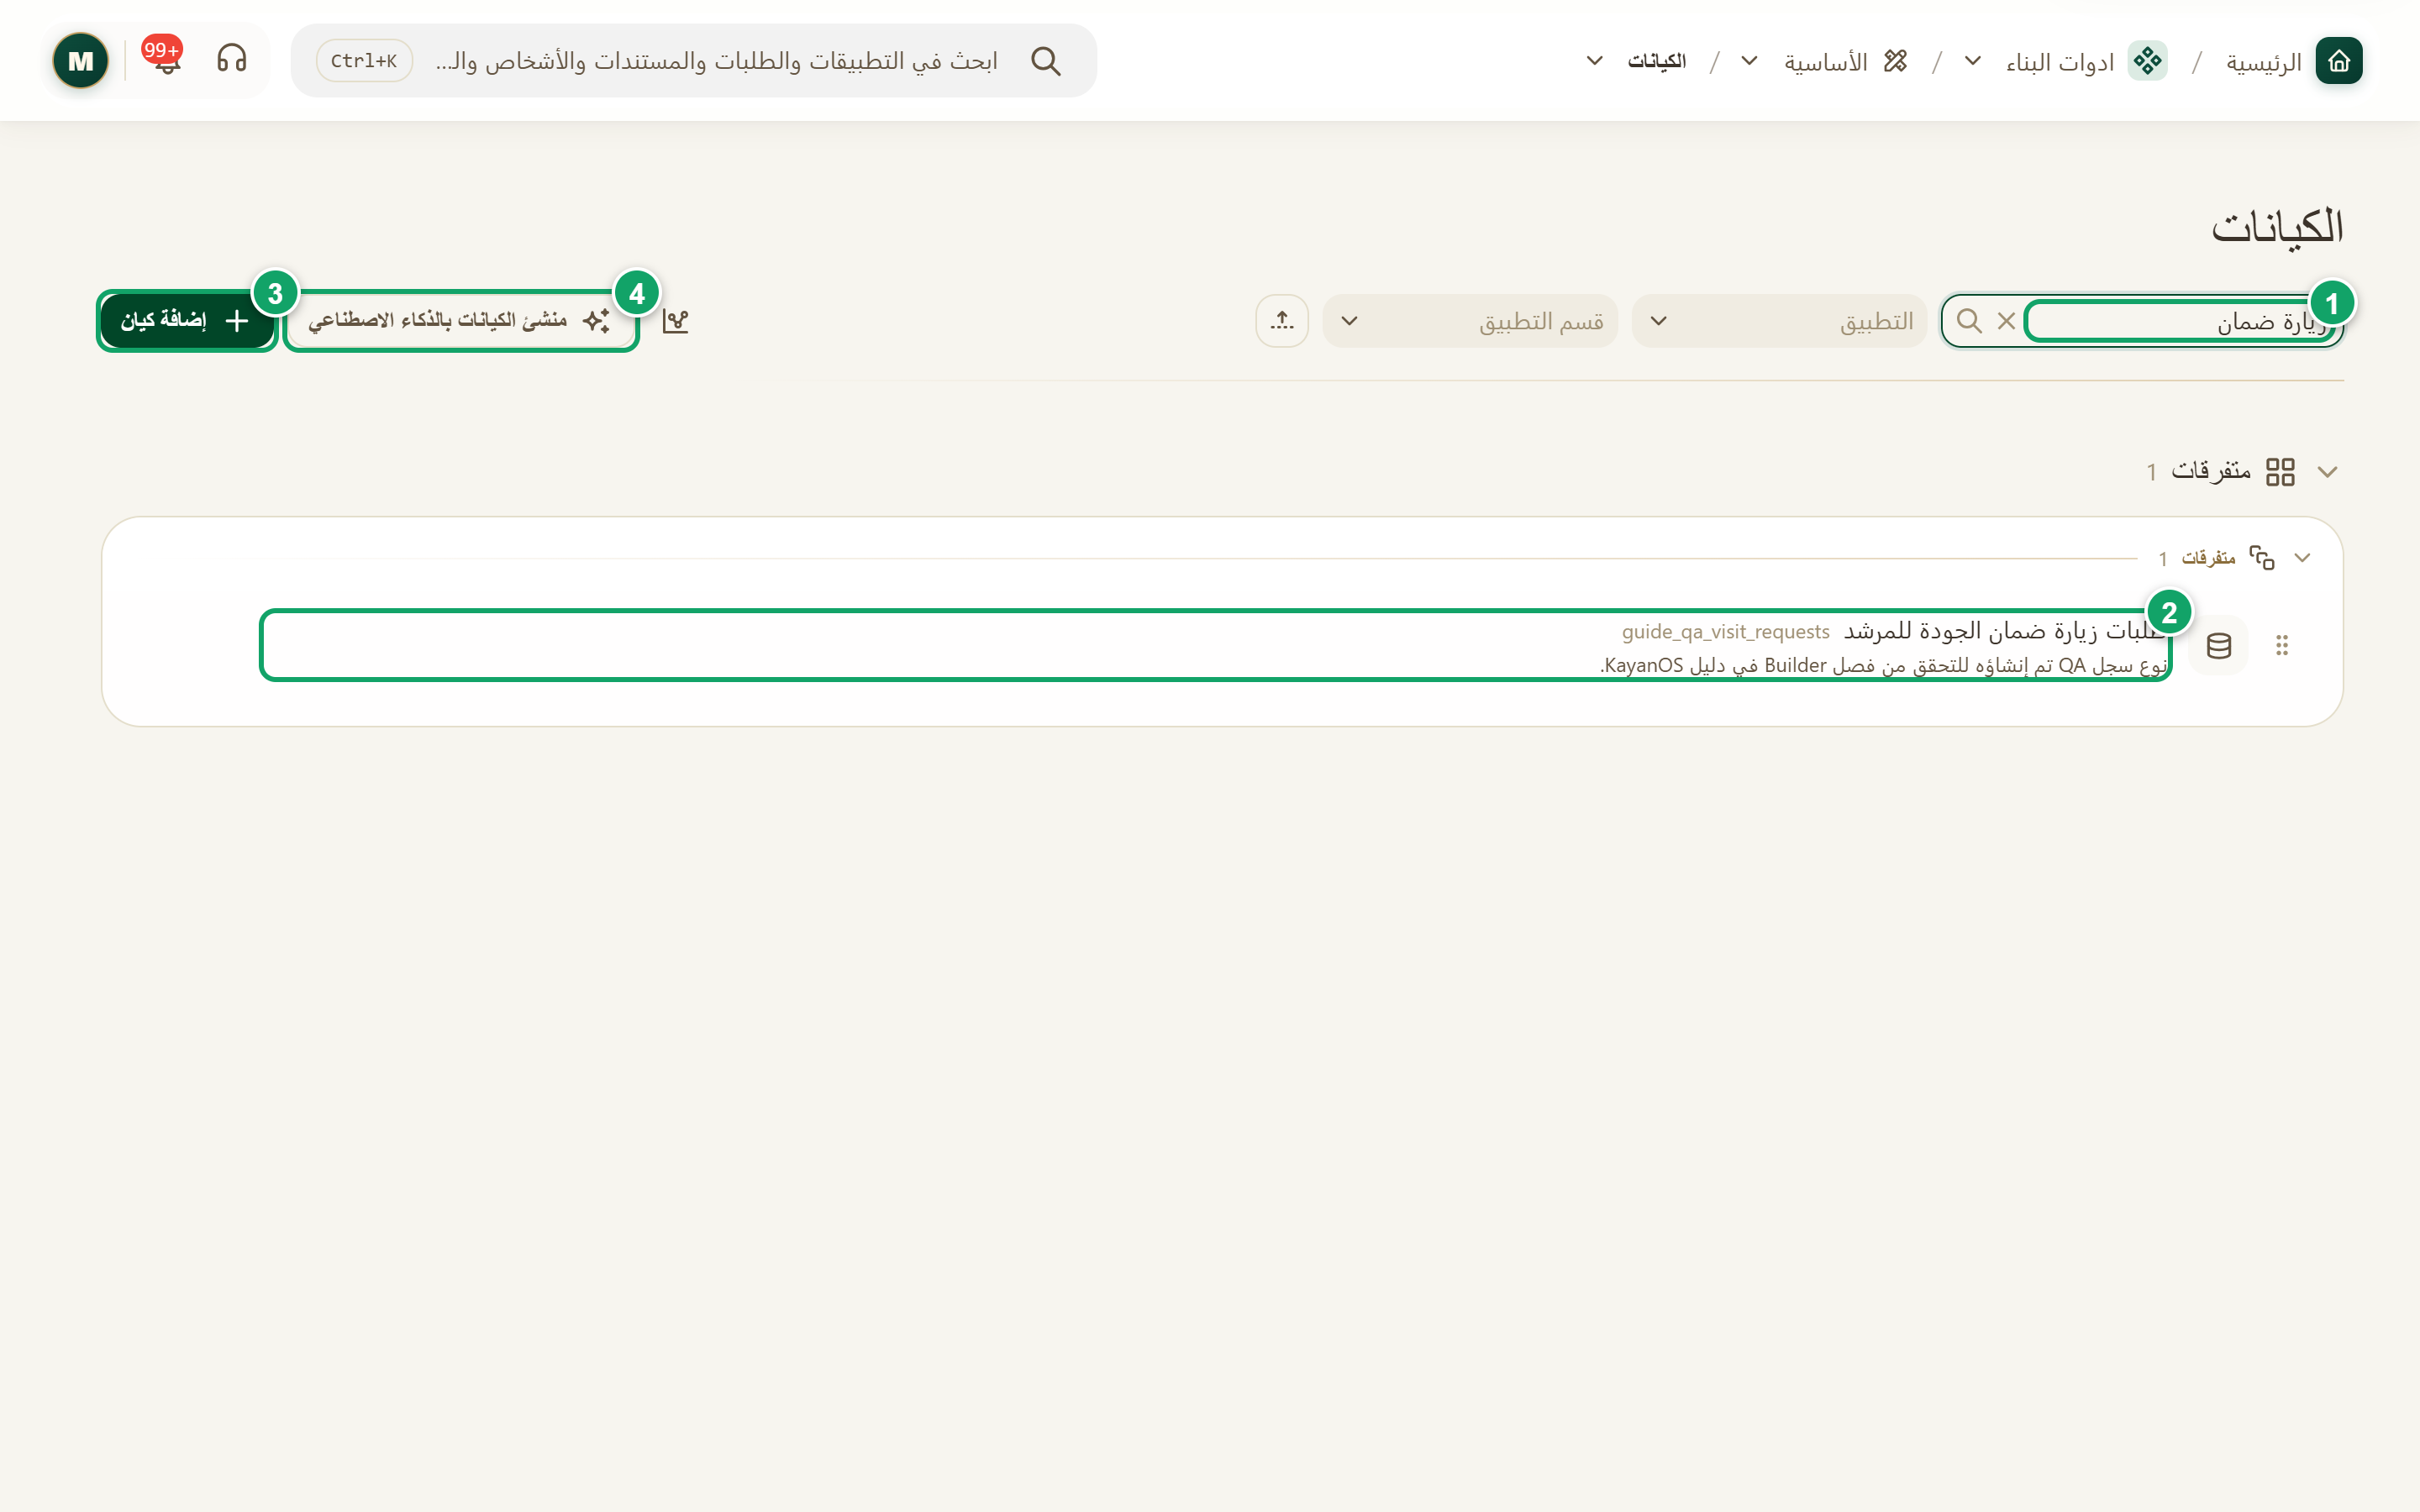
\includegraphics[width=0.95\linewidth,height=0.72\textheight,keepaspectratio]{figures/screens/ch06-entities-ar.png}
\caption{صفحة «الكيانات» بعد البحث عن نوع سجلات}
\label{fig:builder-entities-screen}
\shotnote{تعرض الصفحة أنواع السجلات مجمّعة حسب التطبيق، وهنا ضُيّقت القائمة بالبحث فظهر نوع سجلات اختباري واحد أُنشئ في test2 للتحقق من هذا الفصل. ① مربع البحث: اكتب جزءاً من اسم النوع قبل أن تنشئ نوعاً جديداً. ② النوع الذي وجدته: اضغطه لتفتحه في «المنشئ». ③ «إضافة كيان»: تنشئ نوعاً جديداً عندما لا تجد ما تحتاجه. ④ «منشئ الكيانات بالذكاء الاصطناعي»: يقترح الحقول من وصف تكتبه.}
\end{figure}


\begin{table}[H]
\centering
\caption{ما الذي تجده هنا؟}
\label{tab:builder-entities-data}
\begin{tabularx}{\linewidth}{R{3.6cm} Y}
\rcHeaderRow
\thh{القسم} & \thh{المحتوى والإجراء}\\
قائمة الأنواع & أنواع السجلات مجمّعة حسب التطبيق والقسم، ولكل نوع اسمه ومفتاحه ووصفه. تضيّق القائمة بالبحث أو بفلترَي «التطبيق» و«قسم التطبيق».\\
إضافة كيان & يفتح صفحة تكتب فيها عنوان النوع ووصفه وحقوله الأولى، ثم تضغط «انشاء كيان».\\
منشئ الكيانات بالذكاء الاصطناعي & تصف النوع الذي تريده بكلماتك، فيقترح النظام حقوله لتراجعها قبل الحفظ. يظهر الزر فقط إذا فعّلت المؤسسة الذكاء الاصطناعي في أدوات البناء.\\
عرض مخطط العلاقات & يرسم أنواع السجلات والعلاقات بينها، فتعرف ما يرتبط بالنوع قبل تعديله.\\
فتح نوع موجود & الضغط على النوع يفتحه في «المنشئ»، حيث تعدّل حقوله وصفحته وقوائمه وتنشر التغييرات.\\
\end{tabularx}
\end{table}

\begin{figure}[H]
\centering
\begin{tikzpicture}[node distance=0.5cm]
\node[stepBox] (a) {\RL{البحث عن نوع مشابه}};
\node[stepBox,below=of a] (b) {\RL{إضافة كيان وكتابة عنوانه}};
\node[stepBox,below=of b] (c) {\RL{انشاء كيان}};
\node[stepBox,below=of c] (d) {\RL{فتحه في المنشئ}};
\draw[flowsTo] (a) -- (b);
\draw[flowsTo] (b) -- (c);
\draw[flowsTo] (c) -- (d);
\end{tikzpicture}
\rclegend
\caption{خطوات إنشاء نوع سجلات}
\label{fig:builder-entities-flow}
\shotnote{يبدأ المخطط بالبحث لأن النوع الذي تحتاجه قد يكون موجوداً في تطبيق جاهز، وإنشاء نسخة ثانية منه يفرّق البيانات بين مكانين. وبعد «انشاء كيان» تعود إلى قائمة الكيانات، ثم تفتح النوع الجديد في «المنشئ» لتكمل بناءه، فالإنشاء لا يعني أن التطبيق صار جاهزاً للفريق.}
\end{figure}

\subsection{خطوات العمل والتحقق}
\begin{enumerate}
\item افتح «الكيانات» واكتب في البحث اسماً قريباً مما تحتاجه، ثم راجع النتائج قبل أن تنشئ نوعاً جديداً.
\item اضغط «إضافة كيان»، واكتب عنواناً بصيغة الجمع يصف السجلات، مثل «طلبات الصيانة»، ثم أضف وصفاً قصيراً.
\item سمِّ الحقل الأول المقترح أو غيّر نوعه، واضغط «اضافة حقل جديد» لكل معلومة أساسية أخرى.
\item اضغط زر الإعدادات بجانب «انشاء كيان» لتختار التطبيق والقسم اللذين يظهر فيهما النوع، ثم اضغط «انشاء كيان».
\end{enumerate}

\textbf{تحقق ومعالجة المشكلة:} يجب أن تظهر رسالة نجاح وأن يظهر النوع الجديد في قائمة «الكيانات» تحت التطبيق الذي اخترته. فإذا بقي زر «انشاء كيان» معطلاً، فاكتب عنوان النوع أولاً؛ وإذا لم تجد النوع في القائمة، فأزل فلترَي التطبيق والقسم وابحث باسمه.

\clearpage
\section{الحقول}
\label{sec:builder-feature-fields}

يحدد الحقل معلومة واحدة يحفظها كل سجل، مثل التاريخ أو المبلغ أو الشخص المسؤول. واختيار نوع الحقل المناسب مهم، لأنه يحدد طريقة الإدخال والتحقق من القيمة، ويسمح بالترتيب والتصفية والحساب لاحقاً. وتضيف الحقول من قسم «الحقول» في «المنشئ».

\textbf{المسار ومن يستخدمه:} «الكيانات» ← افتح نوع السجلات ← «الحقول». يستخدمه من يبني نوع السجلات، قبل ترتيب الصفحة والقوائم.

\begin{rcnote}[مثال: شركة الأفق]
يضيف مسؤول النظام إلى «طلبات الزيارة» حقل «معرف تسلسلي» يعطي كل طلب رقماً مثل \en{HZN-VR-0001}، ثم حقل «علاقة» يربط الطلب بالفرع، وحقل «تاريخ» لموعد الزيارة، وحقل «نص طويل» لغرضها. وتطابق خطواته في الصورة الرقمين ① و③.
\end{rcnote}

\begin{figure}[H]
\centering
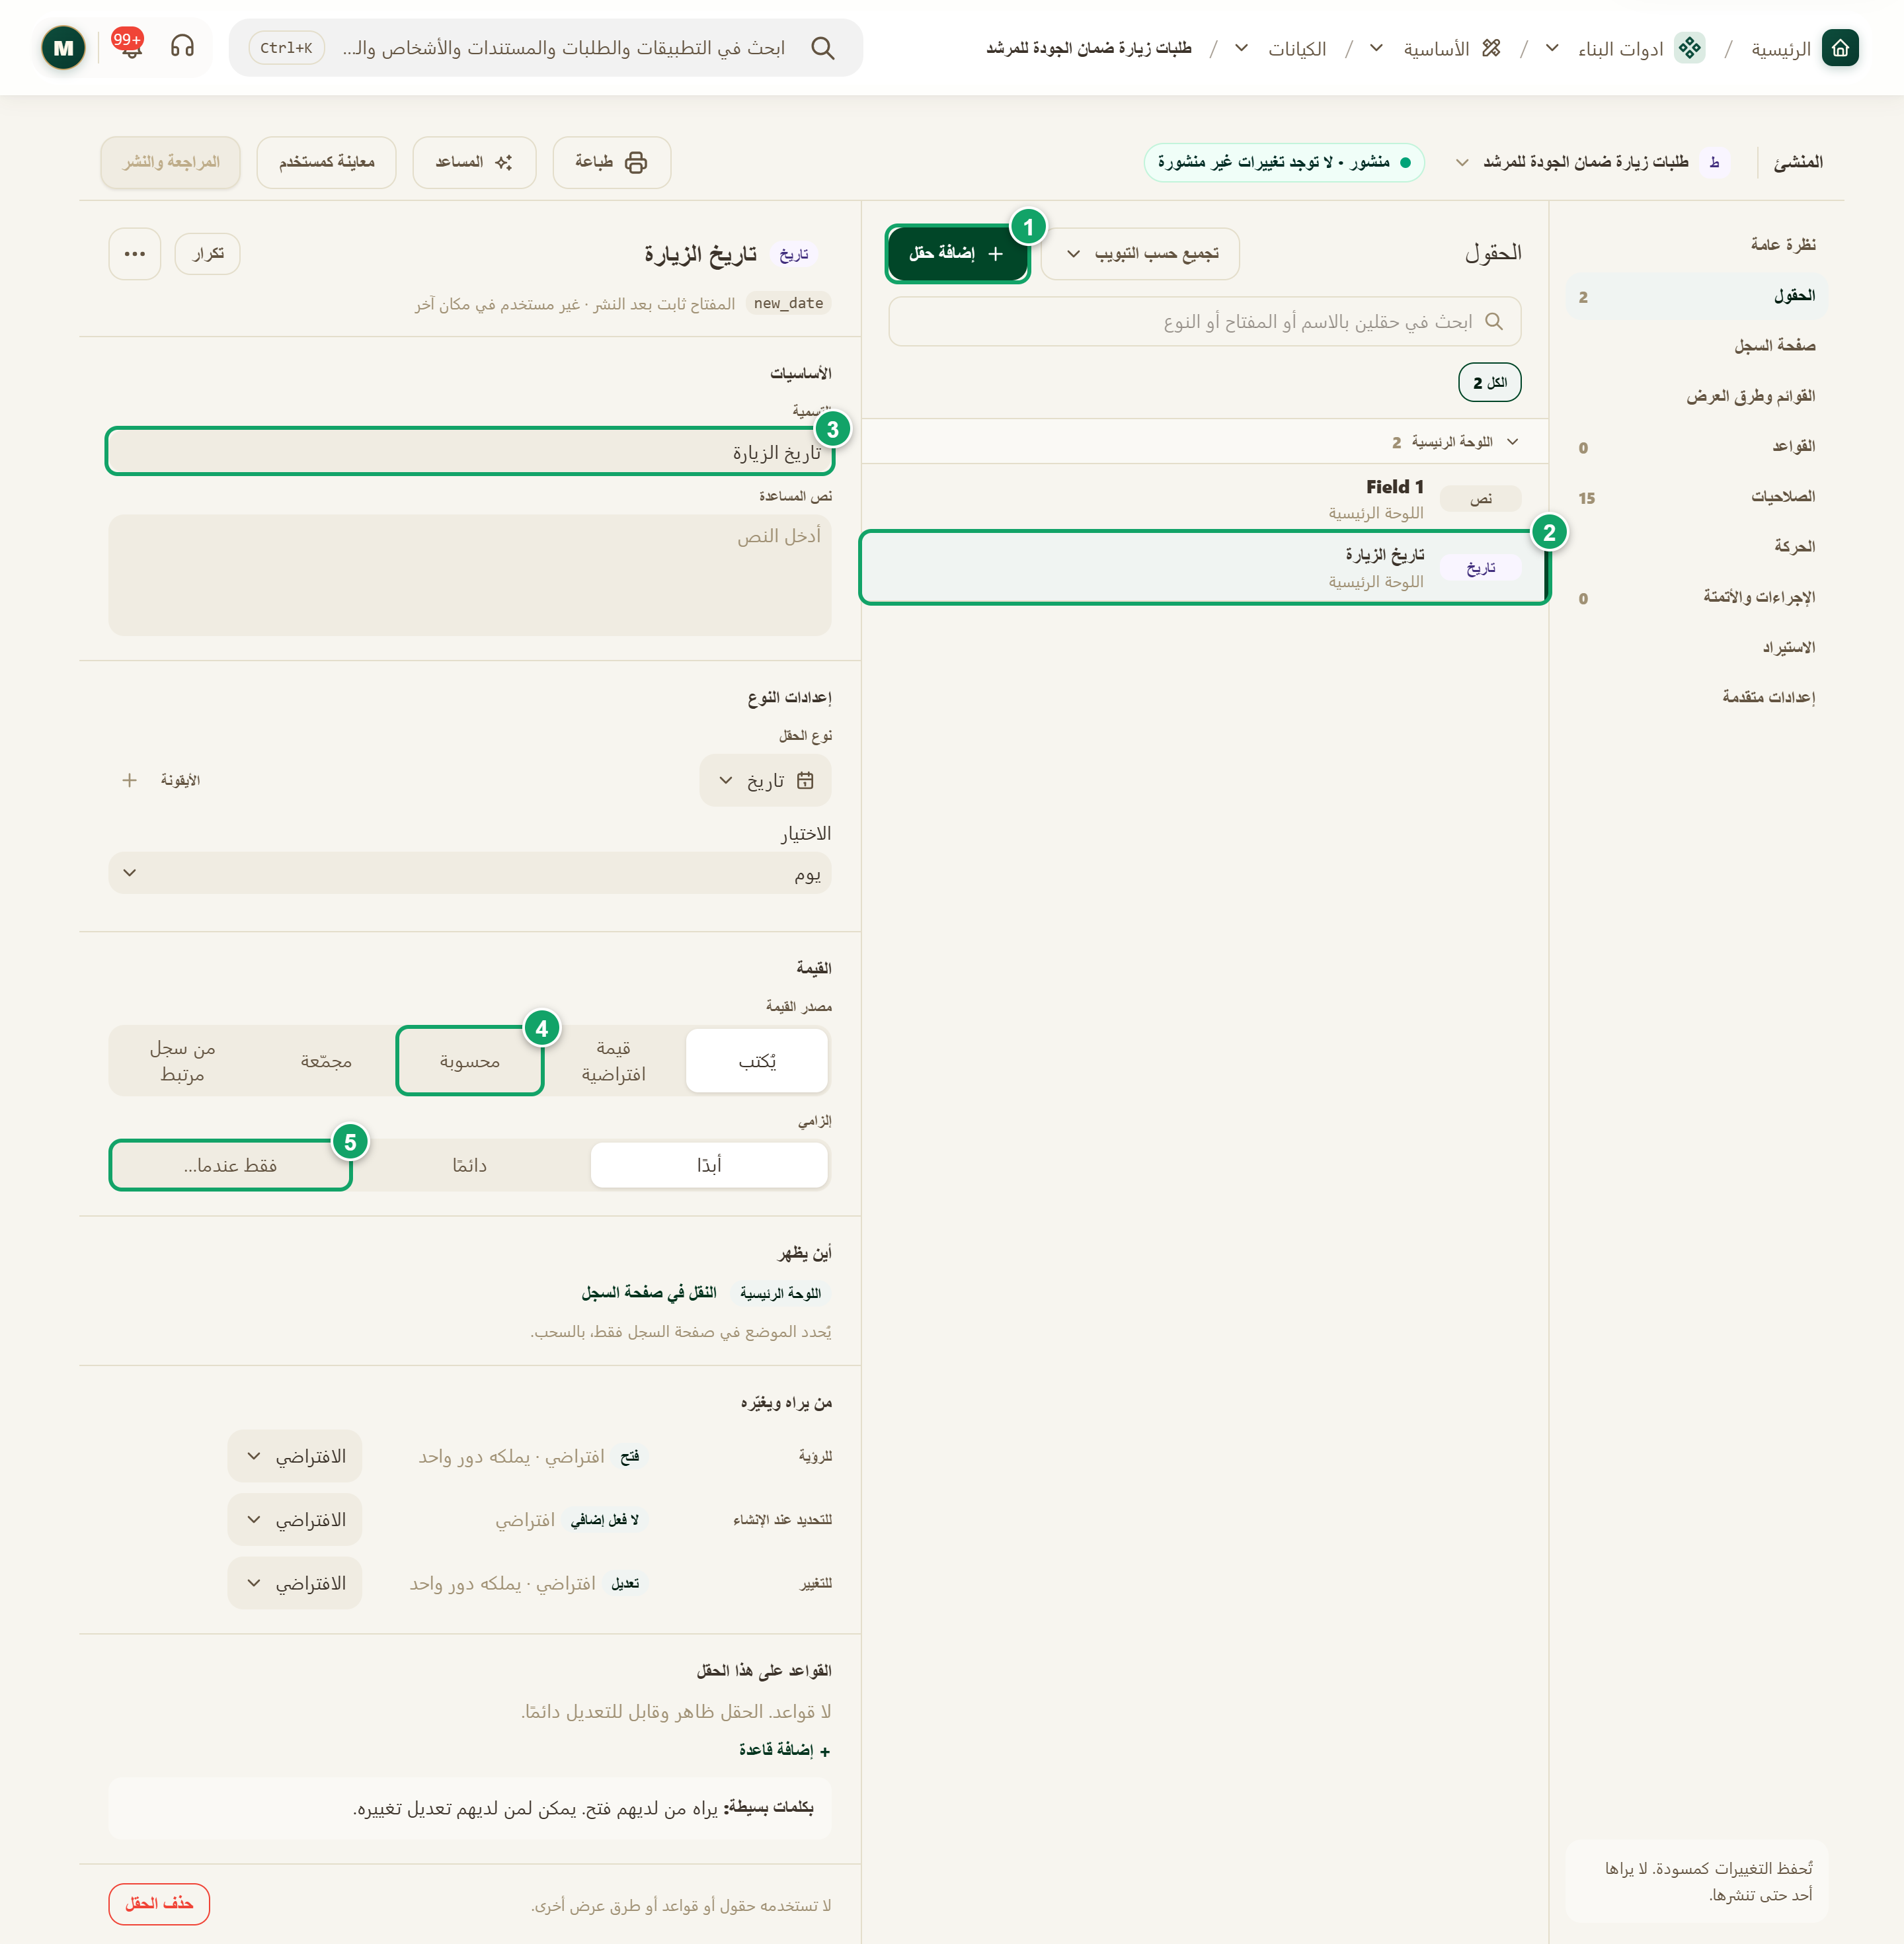
\includegraphics[width=0.95\linewidth,height=0.72\textheight,keepaspectratio]{figures/screens/ch06-ws-fields-ar.png}
\caption{قسم «الحقول» وإعدادات حقل تاريخ}
\label{fig:builder-fields-screen}
\shotnote{يعرض القسم قائمة حقول نوع السجلات، وعند اختيار حقل تظهر إعداداته بجانبه. والحقل المختار هنا حقل «تاريخ» أُضيف ونُشر أثناء اختبار هذا الفصل على test2. ① «إضافة حقل»: تفتح قائمة أنواع الحقول. ② الحقل المختار في القائمة. ③ «التسمية»: الاسم الذي يراه المستخدم. ④ «محسوبة»: تجعل القيمة ناتج صيغة بدلاً من أن يكتبها المستخدم. ⑤ «فقط عندما…»: تجعل الحقل إلزامياً في حالة معينة.}
\end{figure}


\begin{table}[H]
\centering
\caption{أنواع الحقول}
\label{tab:builder-fields-types}
\begin{tabularx}{\linewidth}{R{3.6cm} Y}
\rcHeaderRow
\thh{المجموعة} & \thh{الأنواع ومتى تستخدمها}\\
النصوص & «نص» لقيمة قصيرة، و«نص طويل» للوصف، و«نص منسّق» لنص بتنسيق، و«هاتف» لرقم الهاتف.\\
الأرقام والمعرّفات & «رقم» للكميات والمبالغ، و«المدة» للزمن المستغرق، و«معرف تسلسلي» لرقم مرجعي يولّده النظام لكل سجل.\\
التواريخ والأوقات & «تاريخ» و«تاريخ ووقت» و«وقت»، والنطاقات منها مثل «نطاق التاريخ» عندما يكون للمعلومة بداية ونهاية.\\
الاختيار والحالة & «اختيار» لقائمة قيم محددة، و«قيمة منطقية» لإجابة نعم أو لا، و«الحالة» لمراحل العمل وفق قالب حالات.\\
الملفات والصور & «ملف» للمرفقات، و«صورة رمزية» لصورة تمثّل السجل.\\
الروابط والأشخاص & «علاقة» لربط السجل بسجل من نوع آخر، و«اختيار عضو» لتحديد عضو من المؤسسة.\\
الخرائط & «موقع» لنقطة على الخريطة، و«حدود» لمساحة مرسومة مثل حدود عقار أو منشأة.\\
إجراء & حقل متقدم يعمل مع قسم «الإجراءات والأتمتة».\\
محسوبة ومرتبطة ومجمّعة & قيم لا يكتبها المستخدم: «محسوبة» بصيغة من حقول السجل، و«مرتبطة» تعرض قيمة من سجل مرتبط، و«مجمّعة» تجمع قيم السجلات المرتبطة أو تعدّها.\\
\end{tabularx}
\end{table}

\begin{table}[H]
\centering
\caption{ما الذي تضبطه في كل حقل؟}
\label{tab:builder-fields-settings}
\begin{tabularx}{\linewidth}{R{3.6cm} Y}
\rcHeaderRow
\thh{الإعداد} & \thh{المعنى}\\
التسمية & الاسم الذي يراه المستخدم، ويمكن كتابته بأكثر من لغة.\\
المفتاح & اسم ثابت يستخدمه النظام في الصيغ والقوالب. اختره واضحاً من البداية، لأن الإشارات إليه تعتمد عليه.\\
نص المساعدة & جملة قصيرة تشرح للمستخدم ما يكتبه في الحقل.\\
إلزامي & يمنع حفظ السجل إذا بقي الحقل فارغاً. استخدمه للمعلومات التي لا يكتمل العمل دونها فقط.\\
\end{tabularx}
\end{table}

\begin{figure}[H]
\centering
\begin{tikzpicture}[node distance=0.5cm]
\node[stepBox] (a) {\RL{إضافة حقل}};
\node[stepBox,below=of a] (b) {\RL{اختيار نوع الحقل}};
\node[stepBox,below=of b] (c) {\RL{التسمية والمفتاح}};
\node[stepBox,below=of c] (d) {\RL{الإلزام ونص المساعدة}};
\draw[flowsTo] (a) -- (b);
\draw[flowsTo] (b) -- (c);
\draw[flowsTo] (c) -- (d);
\end{tikzpicture}
\rclegend
\caption{خطوات إضافة حقل}
\label{fig:builder-fields-flow}
\shotnote{يضع المخطط اختيار النوع قبل التسمية، لأن النوع يحدد الإعدادات التي تظهر بعده، مثل خيارات القائمة في «اختيار» أو النوع المرتبط في «علاقة». وتُحفظ كل إضافة في المسودة فوراً، لكن المستخدمين لا يرون الحقل الجديد حتى تنشر التغييرات.}
\end{figure}

\subsection{خطوات العمل والتحقق}
\begin{enumerate}
\item افتح نوع السجلات من «الكيانات»، ثم اختر قسم «الحقول».
\item اضغط «إضافة حقل»، واختر النوع الذي يطابق المعلومة؛ فالتاريخ مثلاً يُحفظ في حقل «تاريخ» لا في «نص».
\item اكتب التسمية وراجع المفتاح، وأضف نص مساعدة عند الحاجة، ثم حدد إن كان الحقل إلزامياً.
\item لحقل يُحسب من غيره، اختر «محسوبة» واكتب الصيغة؛ ولقيمة من سجل مرتبط، اختر «حقل مرتبط» بعد إضافة حقل «علاقة».
\end{enumerate}

\textbf{تحقق ومعالجة المشكلة:} يجب أن يظهر الحقل في قائمة الحقول، وأن تعرض «نظرة عامة» عدده مع الحقول التي لم توضع بعد في أي صفحة. فإذا اخترت نوعاً خاطئاً، فصحّحه قبل النشر وقبل إدخال سجلات حقيقية، لأن تغيير النوع بعد تراكم البيانات أصعب.

\clearpage
\section{صفحة السجل}
\label{sec:builder-feature-record-page}

صفحة السجل هي ما يراه المستخدم عندما يفتح سجلاً واحداً. ويرتّب قسم «صفحة السجل» الحقول في تبويبات وأقسام، فتظهر المعلومات المترابطة معاً بدلاً من قائمة طويلة واحدة. ويمكنك أن تضيف كتلاً في أعلى التبويب الأول، وقوائم بالسجلات المرتبطة.

\textbf{المسار ومن يستخدمه:} نوع السجلات ← «صفحة السجل». يستخدمه من يبني النوع بعد إضافة حقوله.

\begin{rcnote}[مثال: شركة الأفق]
يجعل مسؤول النظام لصفحة طلب الزيارة تبويبين: «الطلب» للفرع والموعد والغرض، و«المراجعة» لملاحظات سارة الخطيب وقرارها، فيجد عمر حداد ما يخصه في التبويب الأول. ويبدأ بإنشاء التبويبين من ② ثم يسحب الحقول إليهما.
\end{rcnote}

\begin{figure}[H]
\centering
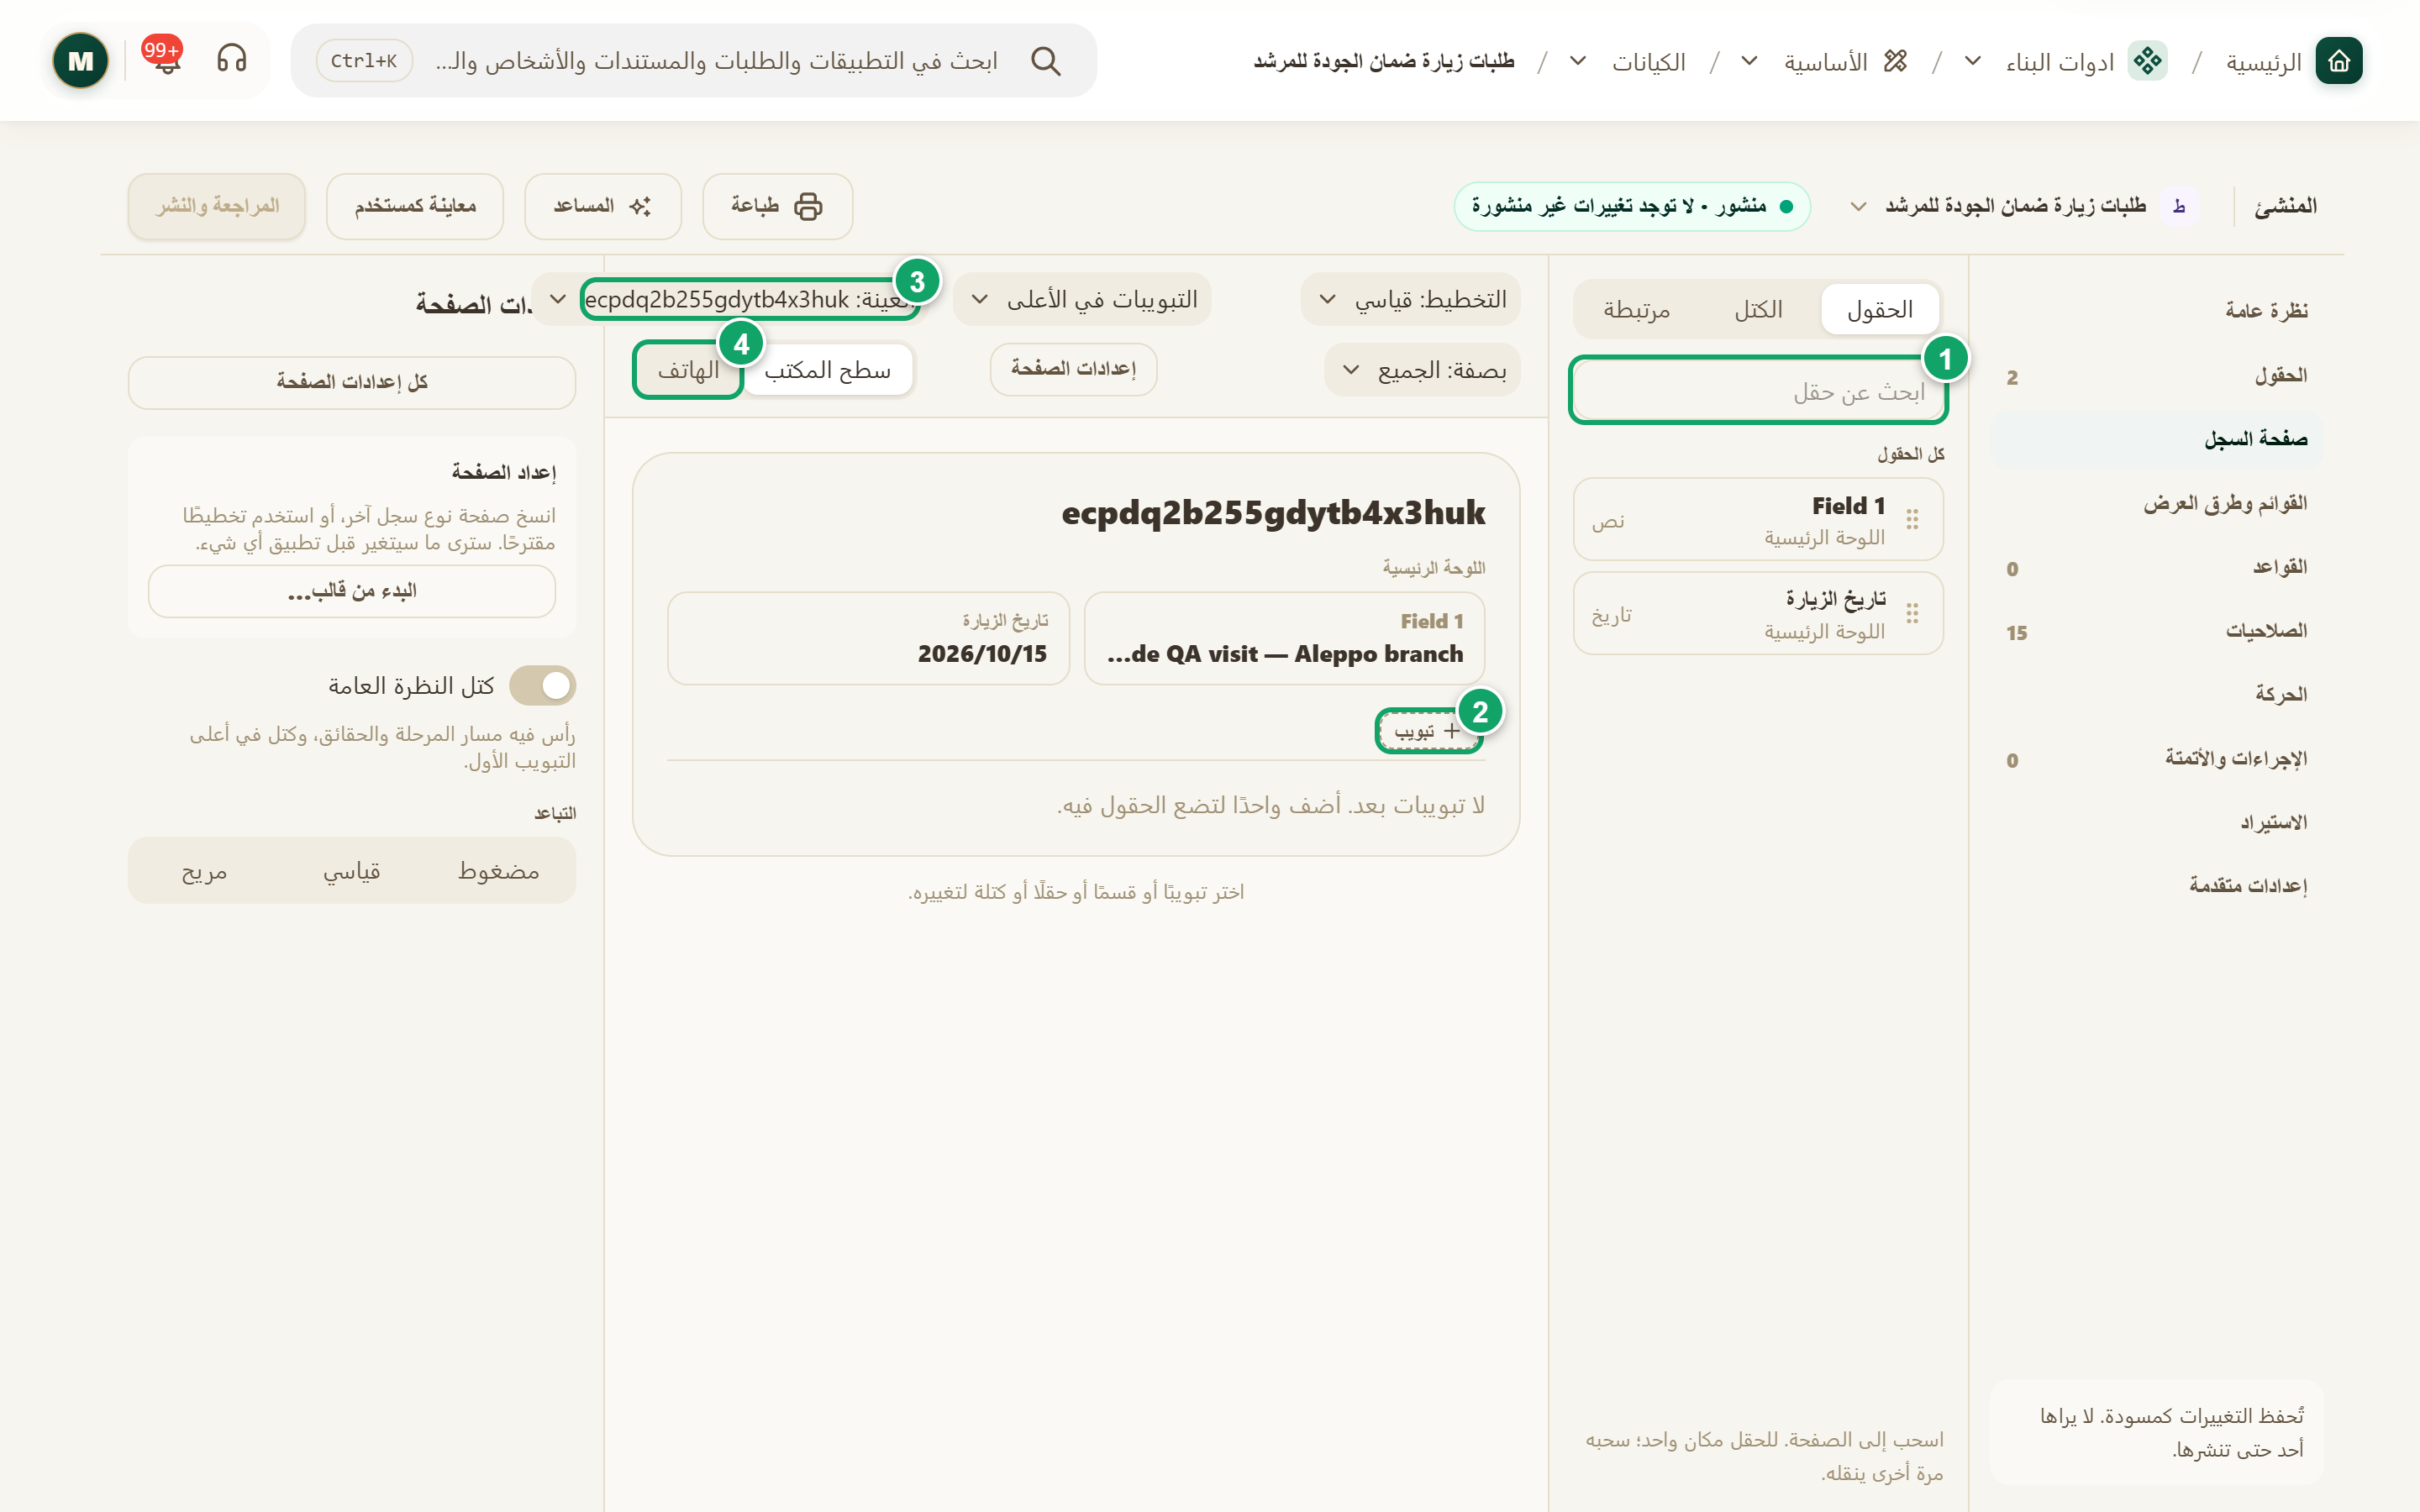
\includegraphics[width=0.95\linewidth,height=0.72\textheight,keepaspectratio]{figures/screens/ch06-ws-record-page-ar.png}
\caption{قسم «صفحة السجل» مع معاينة بسجل حقيقي}
\label{fig:builder-record-page-screen}
\shotnote{يعرض القسم أجزاء الصفحة على جانب، والصفحة نفسها في الوسط بقيم سجل اختباري، فترى أثر الترتيب قبل النشر. ① «ابحث عن حقل»: تجد الحقل الذي تريد سحبه إلى الصفحة. ② «+ تبويب»: يضيف تبويباً تضع فيه الأقسام والحقول. ③ «العينة»: السجل الذي تُعاين به الصفحة. ④ «الهاتف»: يعرض الصفحة كما تظهر على الشاشة الصغيرة.}
\end{figure}


\begin{table}[H]
\centering
\caption{ما الذي تجده هنا؟}
\label{tab:builder-record-page-data}
\begin{tabularx}{\linewidth}{R{3.6cm} Y}
\rcHeaderRow
\thh{القسم} & \thh{المحتوى والإجراء}\\
التبويبات والأقسام & أنشئ «تبويب جديد» أو «قسم جديد»، ثم اسحب الحقول إليها. للحقل مكان واحد في الصفحة، وسحبه مرة أخرى ينقله.\\
أجزاء الصفحة & تجمع «كل الحقول» و«الكتل» والقوائم «المرتبطة»، وتعرض الحقول التي «ليست في الصفحة بعد».\\
التخطيط والرأس & يختار شكل الصفحة: تبويبات أو قائمة أقسام، مع إعدادات الرأس وكتل النظرة العامة.\\
المعاينة & تعرض الصفحة بعينة من سجل حقيقي، كما يراها دور معيّن، على سطح المكتب أو الهاتف.\\
\end{tabularx}
\end{table}

\begin{figure}[H]
\centering
\begin{tikzpicture}[node distance=0.5cm]
\node[entity] (page) {\RL{صفحة السجل}};
\node[entity,below=0.7cm of page] (tab) {\RL{تبويب}};
\node[entity,below=0.7cm of tab] (section) {\RL{قسم}};
\node[entity,below=0.7cm of section] (field) {\RL{حقل}};
\draw[dependsOn] (page) -- (tab);
\draw[dependsOn] (tab) -- (section);
\draw[dependsOn] (section) -- (field);
\end{tikzpicture}
\rclegend
\caption{كيف تُرتّب الصفحة}
\label{fig:builder-record-page-tree}
\shotnote{يوضّح الشكل تدرّج الترتيب: تضم الصفحة تبويبات، ويضم كل تبويب أقساماً، ويضم كل قسم حقولاً. لذلك تنشئ التبويب والقسم أولاً ثم تسحب الحقول إليهما، والحقل الذي لا تضعه في أي قسم يبقى محفوظاً لكنه لا يظهر في الصفحة.}
\end{figure}

\subsection{خطوات العمل والتحقق}
\begin{enumerate}
\item افتح نوع السجلات واختر «صفحة السجل».
\item أنشئ التبويبات التي يحتاجها العمل، ثم أضف قسماً أو أكثر في كل تبويب.
\item اسحب كل حقل من «أجزاء الصفحة» إلى القسم المناسب، وراجع «ليست في الصفحة بعد» حتى لا يبقى حقل مهم خارج الصفحة.
\item غيّر حجم المعاينة إلى «الهاتف» لتتأكد من أن الصفحة واضحة على الشاشة الصغيرة.
\end{enumerate}

\textbf{تحقق ومعالجة المشكلة:} يجب أن تعرض المعاينة الحقول في التبويبات والأقسام التي اخترتها. فإذا لم يظهر حقل، فابحث عنه في «ليست في الصفحة بعد» واسحبه إلى قسم؛ وإذا ظهرت رسالة بأن الحقل موضوع في تبويب غير موجود، فانقله إلى تبويب قائم.

\clearpage
\section{القوائم وطرق العرض}
\label{sec:builder-feature-lists}

يحدد قسم «القوائم وطرق العرض» كيف تظهر سجلات النوع معاً عندما يفتح المستخدم القائمة. فتختار طرق العرض التي يمكن التبديل بينها، مثل «جدول» أو «كانبان» أو «التقويم»، والأعمدة الظاهرة، والأرقام التي تلخّص القائمة في أعلاها.

\textbf{المسار ومن يستخدمه:} نوع السجلات ← «القوائم وطرق العرض». يستخدمه من يبني النوع، ويفيد كل من يتابع السجلات يومياً.

\begin{rcnote}[مثال: شركة الأفق]
يعرض مسؤول النظام طلبات الزيارة في «جدول» بأعمدة الرقم والفرع والموعد والحالة، ويضيف «التقويم» حسب موعد الزيارة، فترى سارة الخطيب زيارات الأسبوع في نظرة واحدة. ويبدأ بتفعيل المفتاح ① لاختيار الجدول والتقويم.
\end{rcnote}

\begin{figure}[H]
\centering
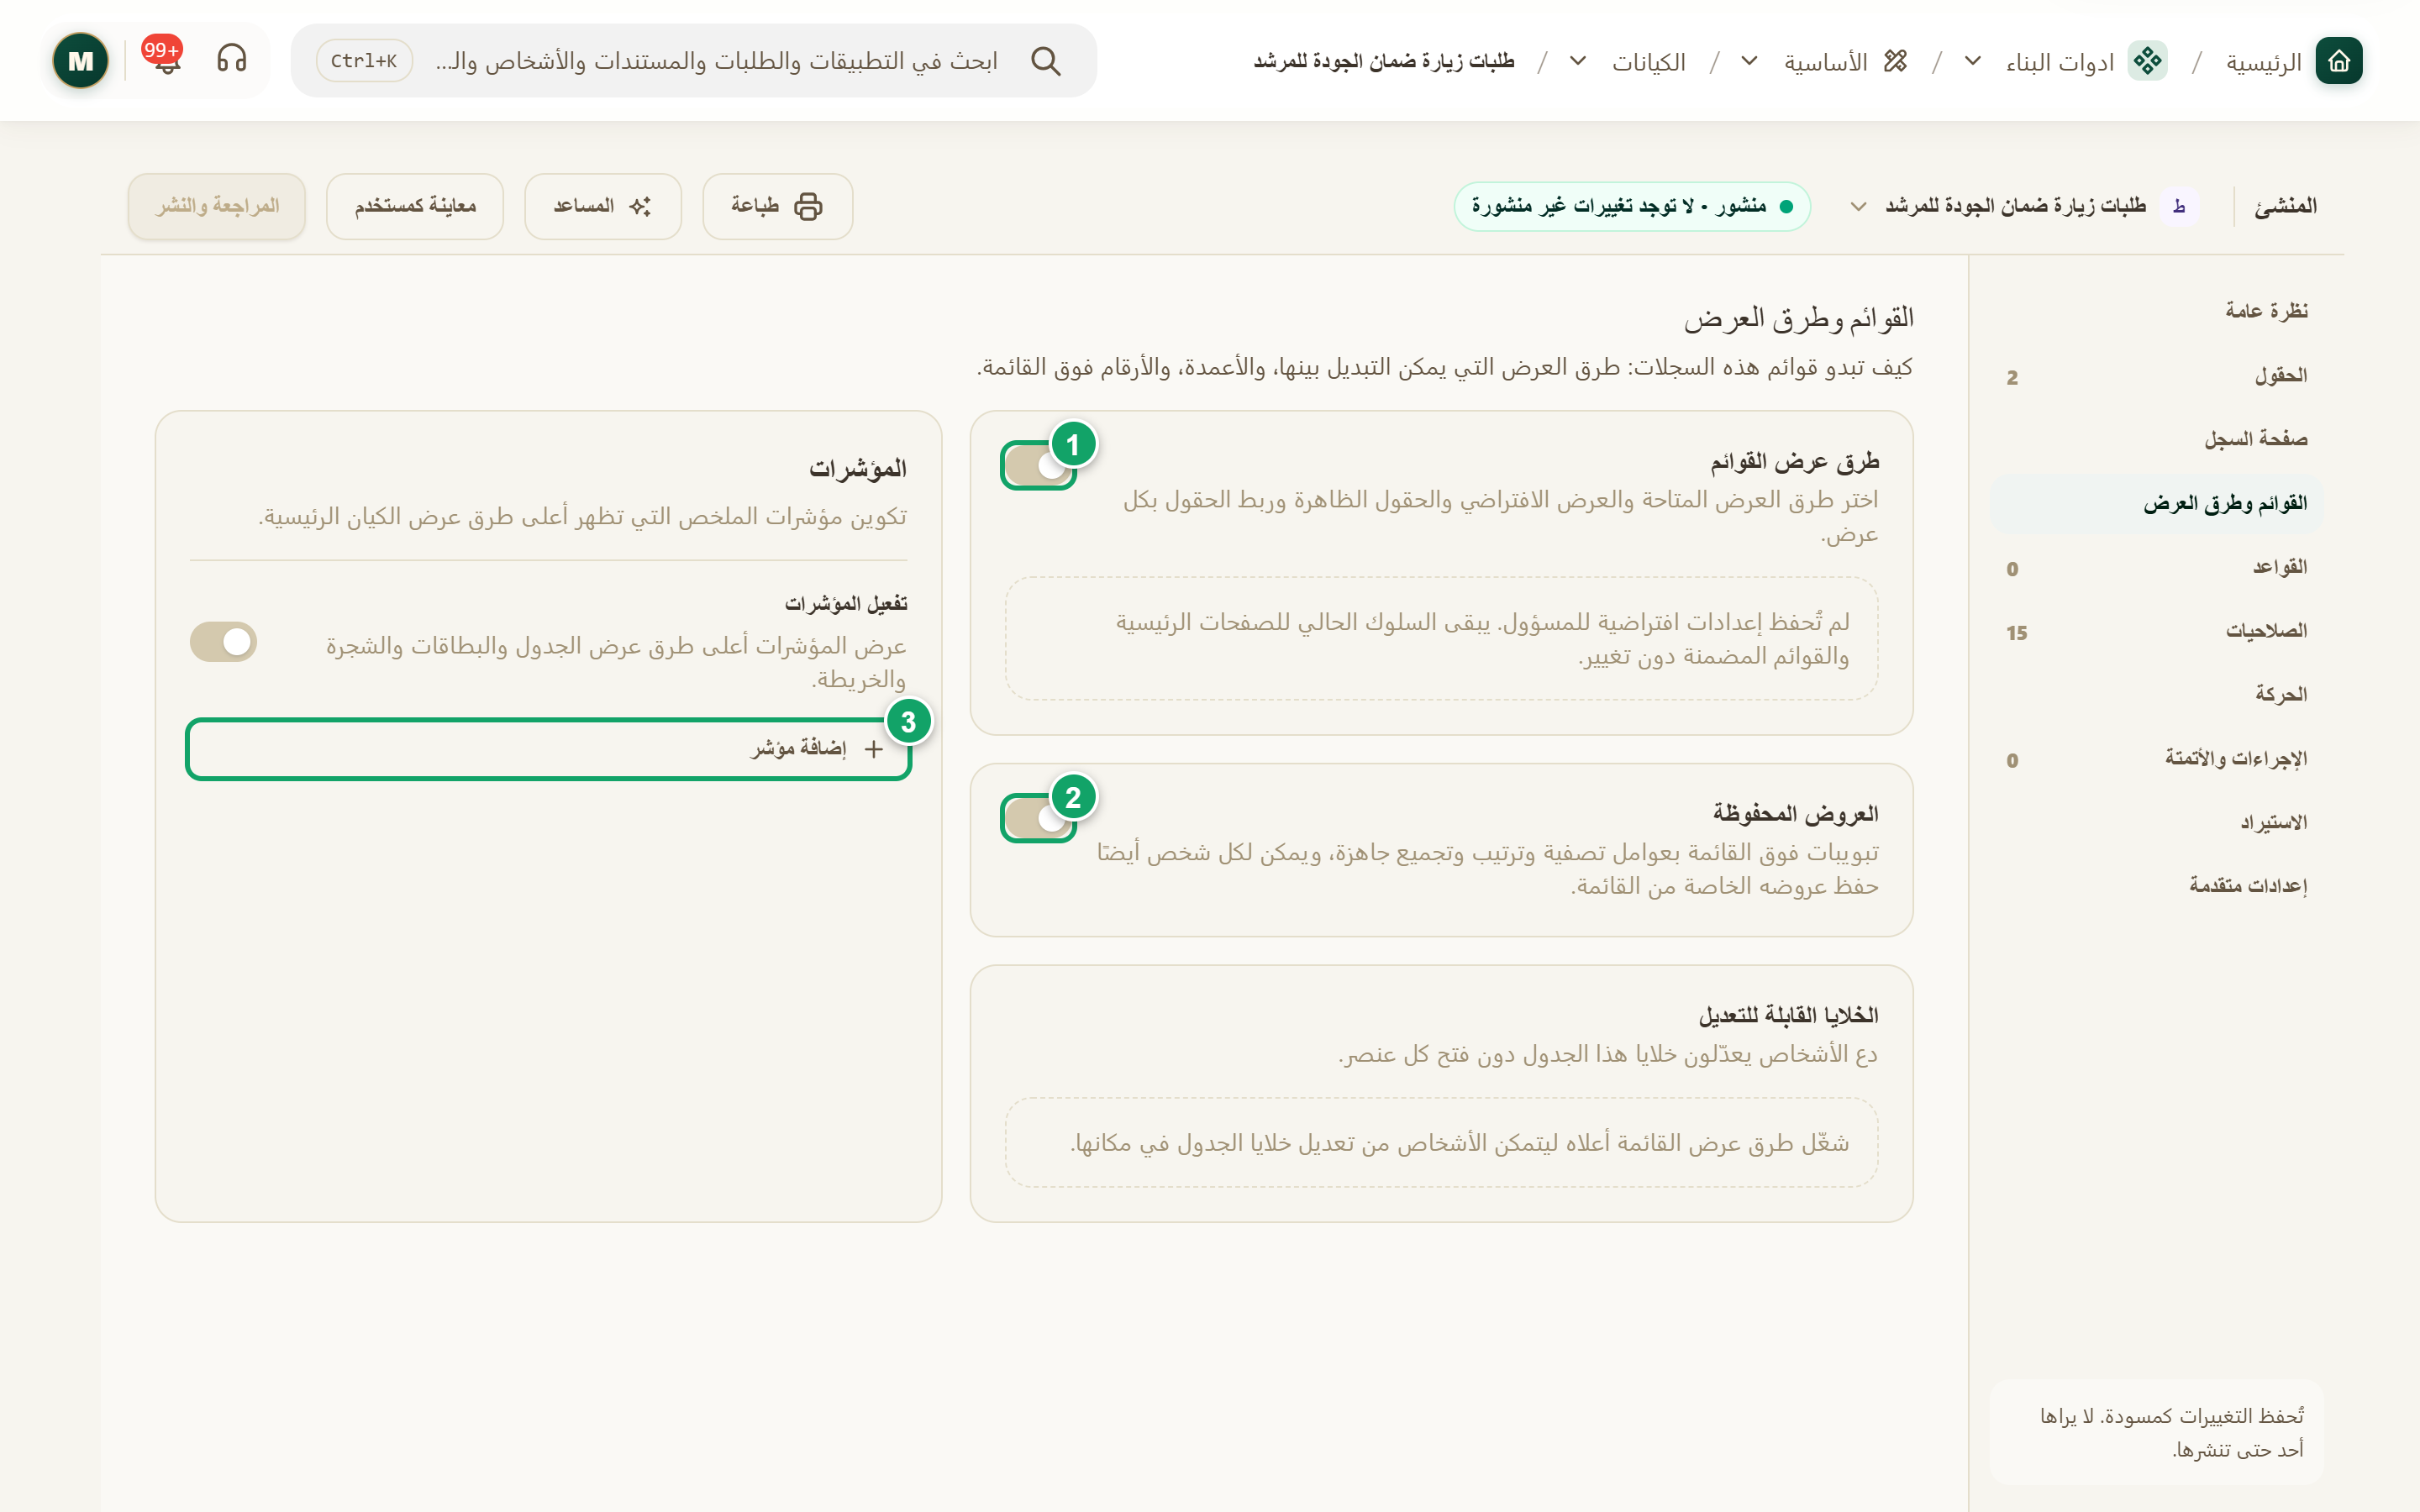
\includegraphics[width=0.95\linewidth,height=0.72\textheight,keepaspectratio]{figures/screens/ch06-ws-lists-ar.png}
\caption{قسم «القوائم وطرق العرض»}
\label{fig:builder-lists-screen}
\shotnote{يجمع القسم ما يتحكم في شكل قائمة السجلات. وكل المفاتيح متوقفة هنا، فتعمل القائمة بإعدادها الافتراضي. ① مفتاح «طرق عرض القوائم»: يتيح اختيار طرق العرض المتاحة والافتراضية والأعمدة. ② مفتاح «العروض المحفوظة»: يضيف تبويبات جاهزة فوق القائمة. ③ «إضافة مؤشر»: يضيف رقماً ملخصاً فوق القائمة.}
\end{figure}

\begin{figure}[H]
\centering
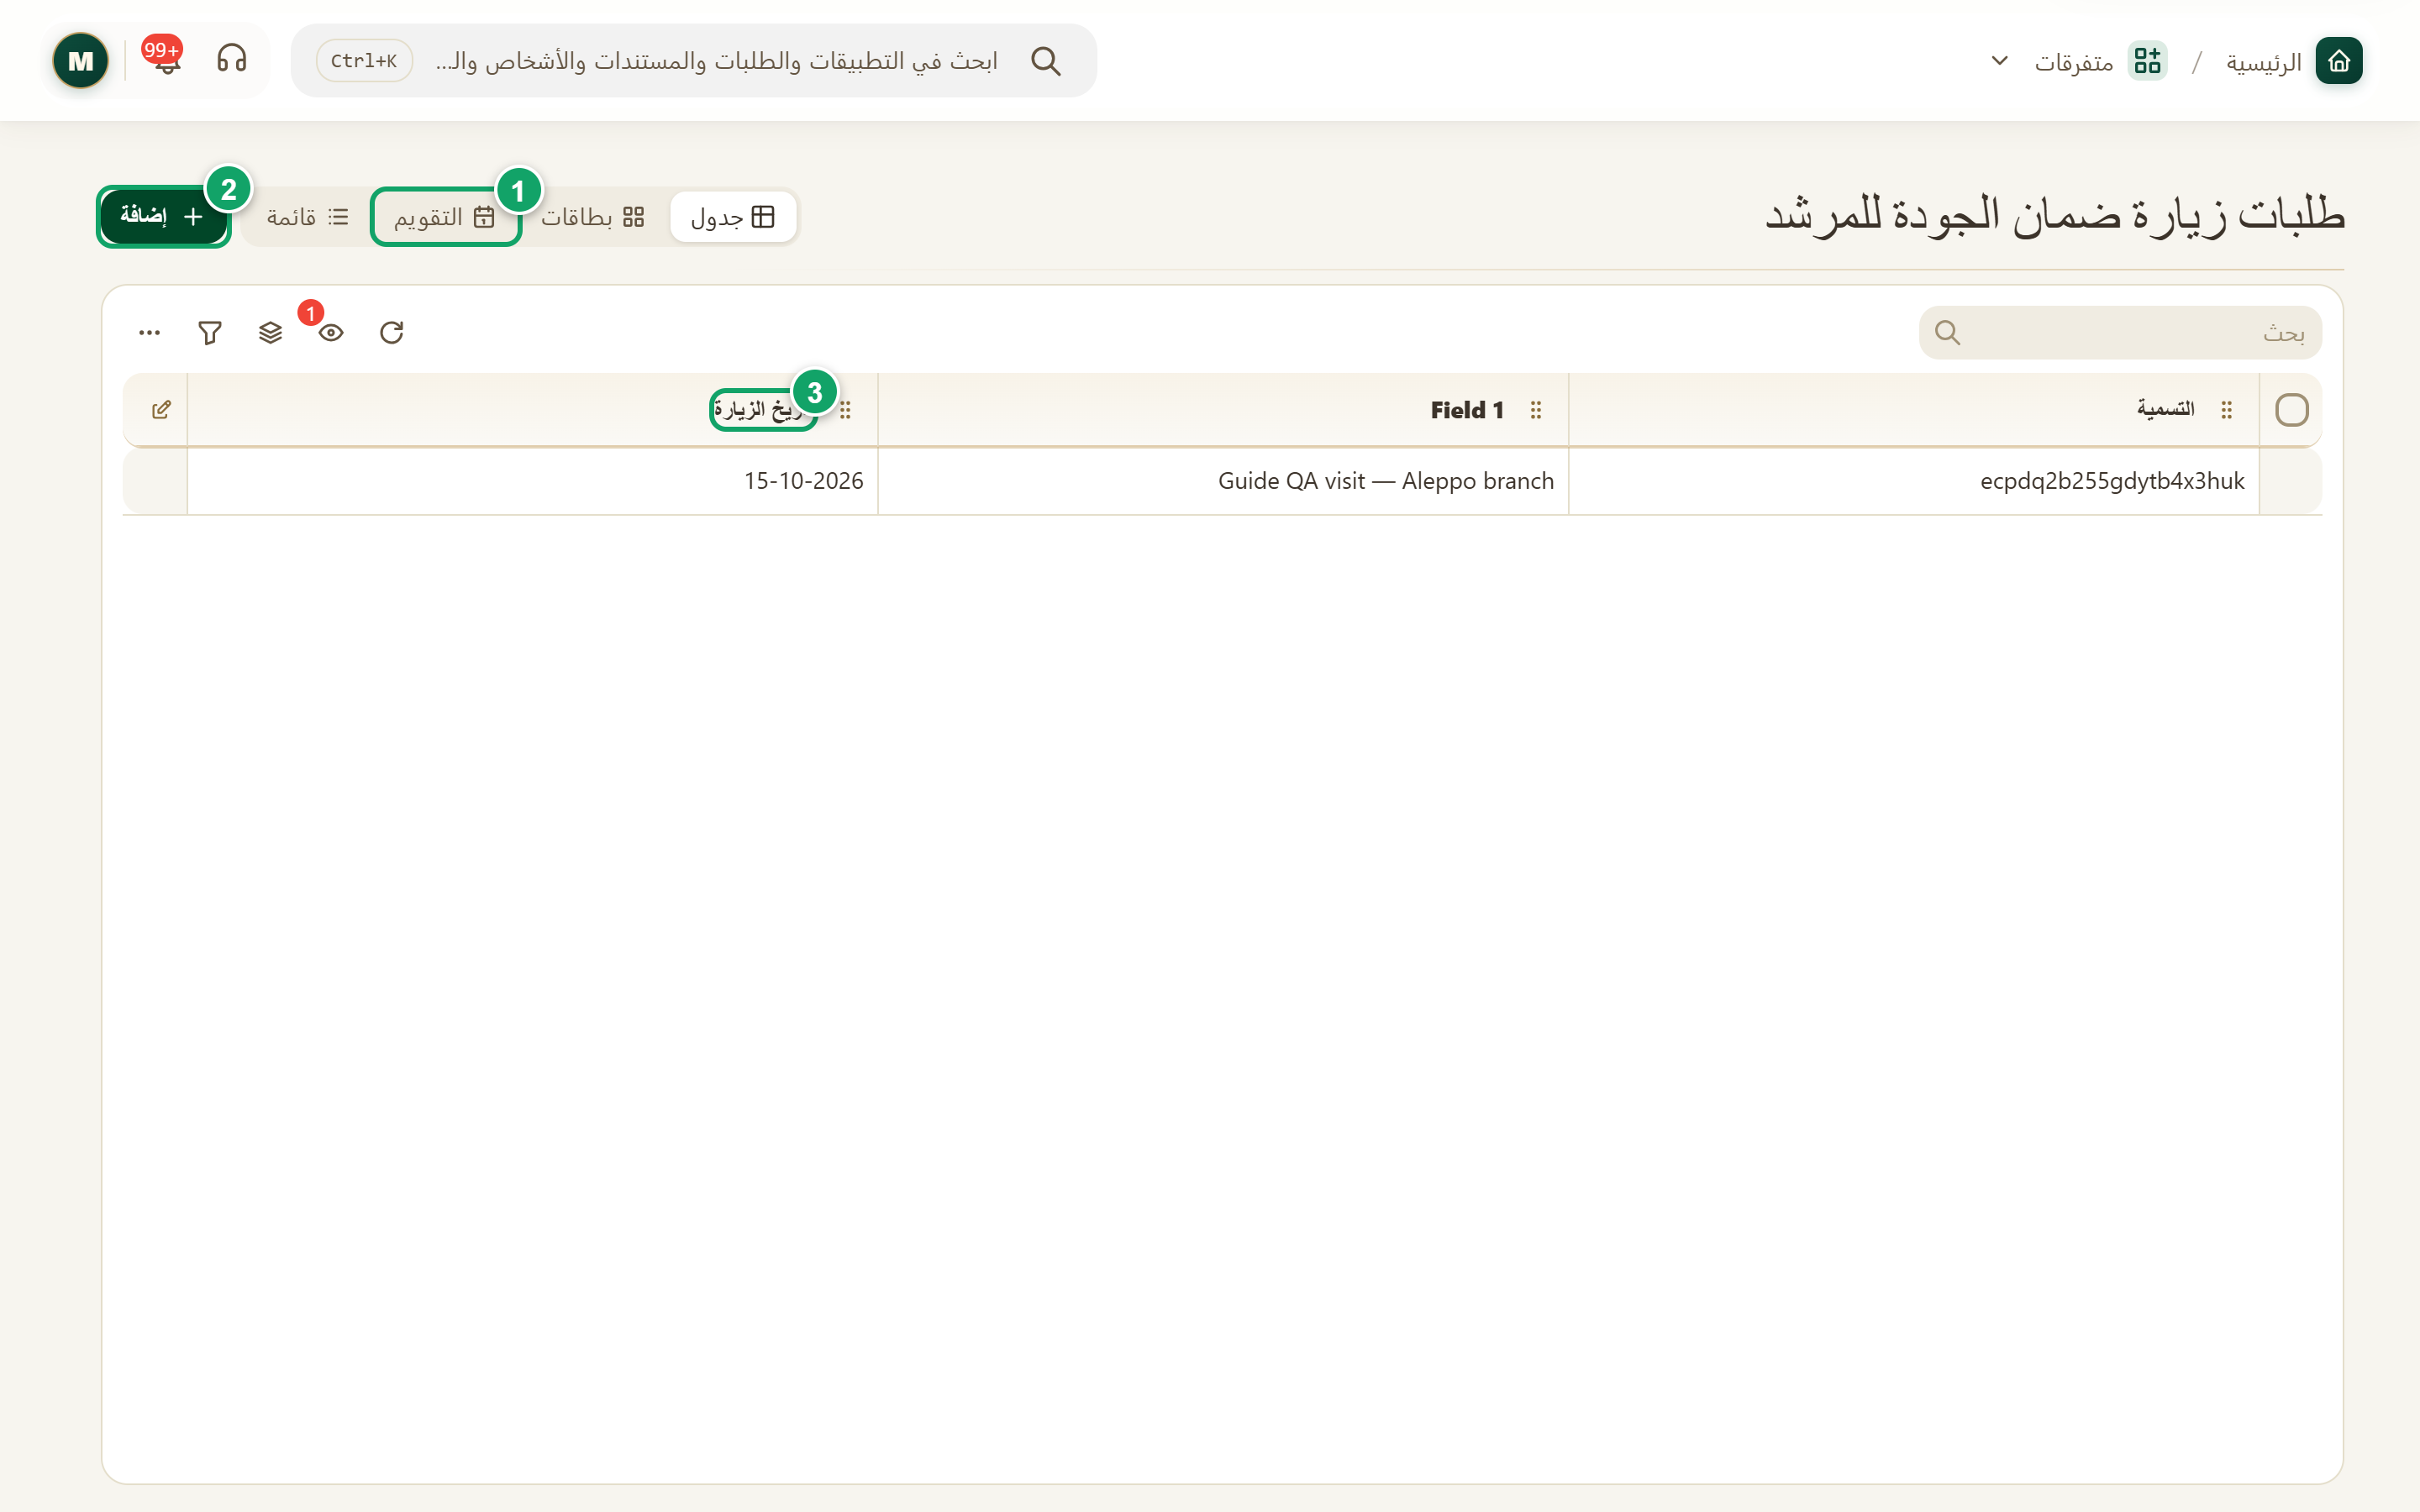
\includegraphics[width=0.95\linewidth,height=0.72\textheight,keepaspectratio]{figures/screens/ch06-records-ar.png}
\caption{قائمة سجلات النوع بعد النشر}
\label{fig:builder-lists-records}
\shotnote{هذه هي القائمة التي يراها المستخدمون بعد النشر، وفيها سجل اختبار أُنشئ في test2 ثم أُعيد فتحه للتحقق من الحفظ. ① «التقويم»: ظهرت طريقة العرض هذه لأن للنوع حقل تاريخ. ② «إضافة»: تنشئ سجلاً جديداً. ③ عمود «تاريخ الزيارة»: يعرض القيمة المحفوظة للسجل الاختباري بعد إعادة فتحه.}
\end{figure}


\begin{table}[H]
\centering
\caption{طرق العرض المتاحة}
\label{tab:builder-lists-modes}
\begin{tabularx}{\linewidth}{R{3.6cm} Y}
\rcHeaderRow
\thh{طريقة العرض} & \thh{متى تناسب}\\
جدول وقائمة & متاحان دائماً لمراجعة السجلات ومقارنتها صفاً صفاً، مع الترتيب والتصفية.\\
بطاقات ومعرض & «بطاقات» متاحة دائماً، أما «معرض» فيظهر عندما يكون للنوع حقل صورة.\\
كانبان & يوزّع السجلات في أعمدة حسب الحالة أو قيمة اختيار، ويظهر عندما يوجد حقل مناسب لذلك.\\
التقويم والخط الزمني & يظهران عندما يكون للنوع حقل تاريخ أو نطاق زمني، مثل المواعيد والمراحل.\\
خريطة & تظهر عندما يكون للنوع حقل «موقع» أو «حدود».\\
شجرة & تظهر عندما تفعّل «السجلات الأم» في «إعدادات متقدمة»، فتُعرض السجلات في تسلسل أب وأبناء.\\
\end{tabularx}
\end{table}

\begin{figure}[H]
\centering
\begin{tikzpicture}[node distance=0.5cm]
\node[entity] (fields) {\RL{الحقول}};
\node[entityOpt,below right=0.7cm and 0.3cm of fields] (cal) {\RL{التقويم}};
\node[entityOpt,below left=0.7cm and 0.3cm of fields] (map) {\RL{خريطة}};
\draw[dependsOnOpt] (fields.south) -- ++(0,-0.3) -| (cal.north);
\draw[dependsOnOpt] (fields.south) -- ++(0,-0.3) -| (map.north);
\end{tikzpicture}
\rclegend
\caption{طرق عرض تعتمد على نوع الحقل}
\label{fig:builder-lists-depends}
\shotnote{يوضّح الشكل أن بعض طرق العرض تحتاج إلى حقل من نوع معيّن: فالتقويم يحتاج إلى تاريخ، والخريطة تحتاج إلى موقع أو حدود. لذلك إذا لم تجد طريقة عرض تريدها، فراجع الحقول أولاً، لأن الطريقة لا تظهر في الخيارات دون الحقل الذي تعتمد عليه.}
\end{figure}

\subsection{خطوات العمل والتحقق}
\begin{enumerate}
\item افتح نوع السجلات واختر «القوائم وطرق العرض».
\item فعّل طرق العرض التي يحتاجها الفريق، واختر الطريقة الافتراضية التي تظهر أولاً.
\item اختر الأعمدة الظاهرة ورتّبها حسب أهميتها للعمل اليومي، وأضف الأرقام الملخّصة عند الحاجة.
\end{enumerate}

\textbf{تحقق ومعالجة المشكلة:} يجب أن تعرض «نظرة عامة» الطريقة الافتراضية وعدد العروض المحفوظة. وبعد النشر افتح قائمة السجلات وبدّل بين الطرق للتأكد منها؛ فإذا كانت طريقة العرض فارغة، فتحقق من أن السجلات تحمل قيمة في الحقل الذي تعتمد عليه.

\clearpage
\section{القواعد}
\label{sec:builder-feature-rules}

القاعدة تجعل السجل يتصرف بحسب ما فيه من قيم، دون أن يتذكر المستخدم ذلك بنفسه. فقد تُظهر حقلاً عند اختيار قيمة معينة، أو تقفله بعد الإنشاء، أو تجعله إلزامياً في حالة محددة، أو ترفض قيمة غير منطقية. ويجمع قسم «القواعد» هذه القواعد كلها في قائمة واحدة.

\textbf{المسار ومن يستخدمه:} نوع السجلات ← «القواعد». يستخدمه من يبني النوع، بعد أن تكتمل الحقول.

\begin{rcnote}[مثال: شركة الأفق]
يضيف مسؤول النظام قاعدة تُظهر حقل «سبب الرفض» عندما تكون الحالة «مرفوض» فقط، وقاعدة تتحقق من أن موعد الزيارة يقع في تاريخ الطلب أو بعده. ويضيف القاعدتين من ①.
\end{rcnote}

\begin{figure}[H]
\centering
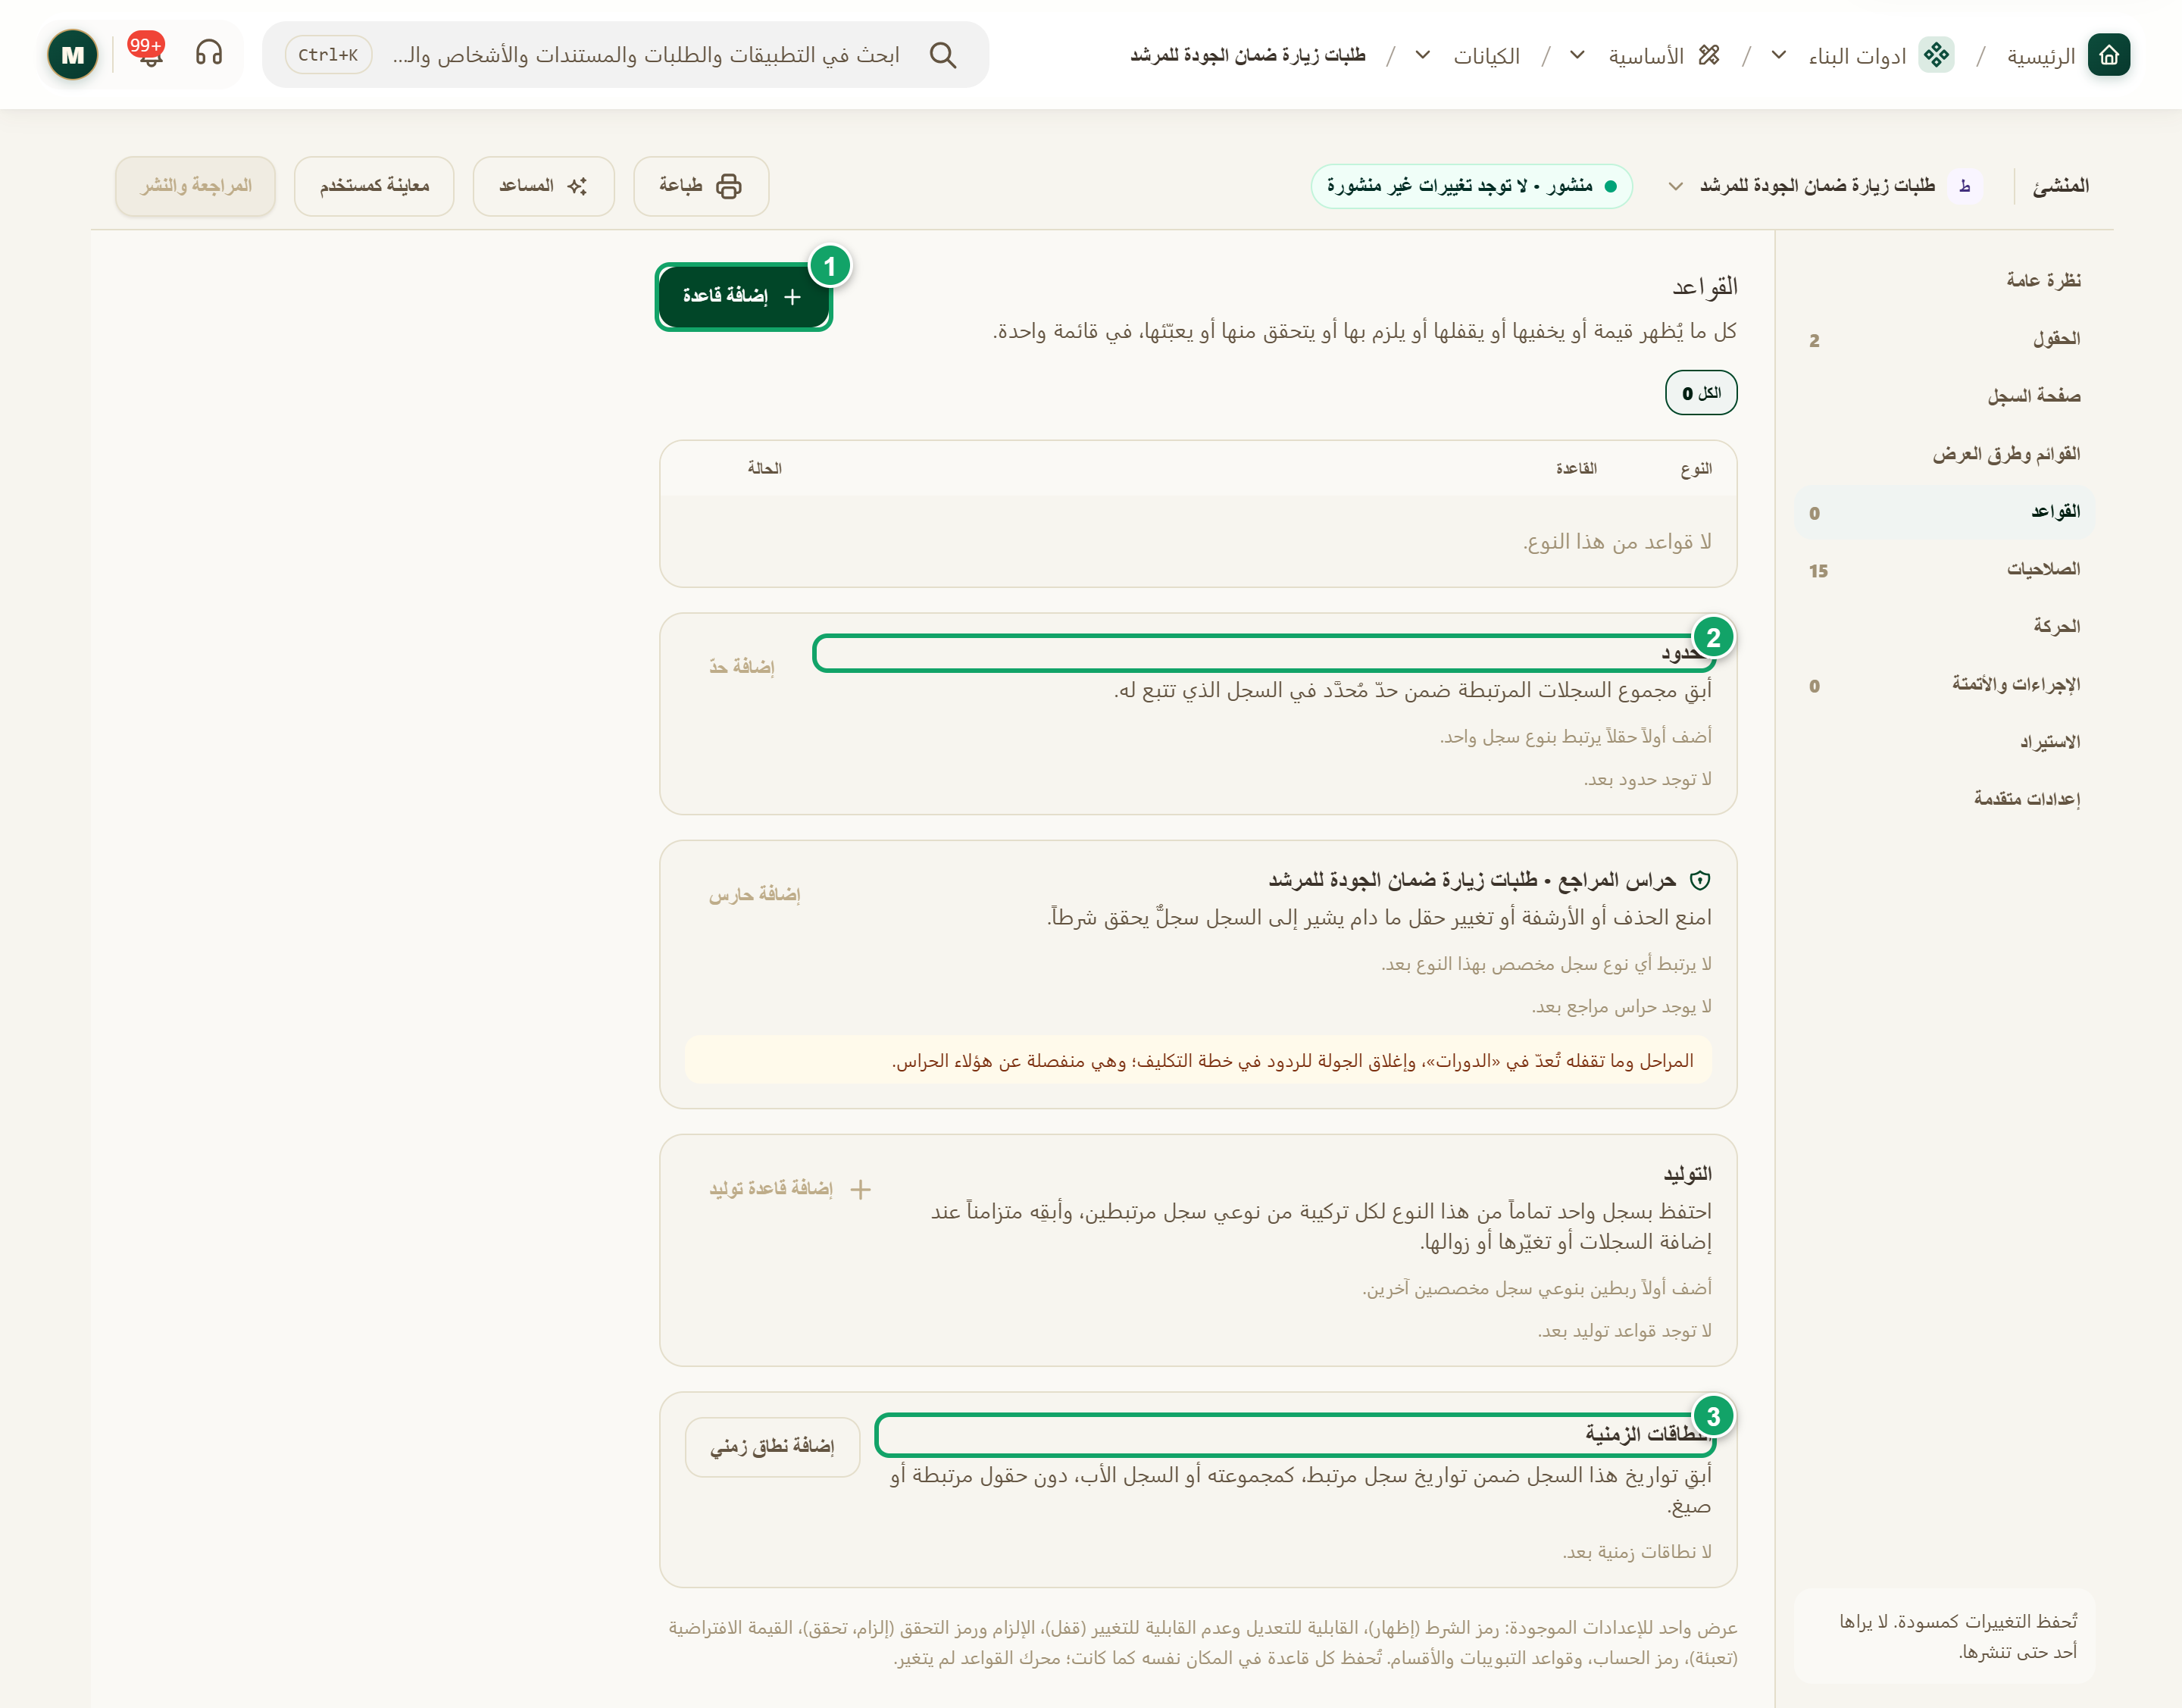
\includegraphics[width=0.95\linewidth,height=0.72\textheight,keepaspectratio]{figures/screens/ch06-ws-rules-ar.png}
\caption{قسم «القواعد» وأدواته الإضافية}
\label{fig:builder-rules-screen}
\shotnote{تظهر في أعلى القسم قائمة القواعد، وتحتها أدوات أخرى تحمي البيانات، مثل الحدود والنطاقات الزمنية. والقائمة فارغة لأن النوع الاختباري بلا قواعد. ① «إضافة قاعدة»: تفتح محرر القاعدة. ② «الحدود»: تُبقي مجموع السجلات المرتبطة ضمن حدّ. ③ «النطاقات الزمنية»: تُبقي تواريخ السجل ضمن تواريخ سجل مرتبط.}
\end{figure}


\begin{table}[H]
\centering
\caption{أنواع القواعد}
\label{tab:builder-rules-kinds}
\begin{tabularx}{\linewidth}{R{3.6cm} Y}
\rcHeaderRow
\thh{النوع} & \thh{ماذا تفعل؟}\\
إظهار أو إخفاء & تُظهر حقلاً أو تبويباً أو قسماً عندما يتحقق شرط، وتخفيه في غير ذلك.\\
قفل التعديل & تمنع تغيير حقل أو تبويب أو قسم: «مقفل عندما» يتحقق شرط، أو «قابل للتعديل فقط عندما»، أو «بعد الإنشاء».\\
إلزام & تجعل الحقل إلزامياً «دائمًا» أو «فقط عندما» يتحقق شرط، مع رسالة توضح السبب.\\
تحقق من القيمة & ترفض القيمة إن لم تكن، مثلاً، أكبر من رقم أو بعد تاريخ أو مختلفة عن حقل آخر، وتعرض رسالتك.\\
تعبئة قيمة & تبدأ الحقل بقيمة جاهزة يستطيع المستخدم تغييرها.\\
حساب & تعرض الحقول المحسوبة؛ وتعديلها يتم من قسم «الحقول».\\
\end{tabularx}
\end{table}

\begin{table}[H]
\centering
\caption{قواعد أخرى ليست في هذا القسم}
\label{tab:builder-rules-other}
\begin{tabularx}{\linewidth}{R{3.6cm} Y}
\rcHeaderRow
\thh{القاعدة} & \thh{أين تجدها؟}\\
الحدود & أسفل قائمة القواعد: تُبقي مجموع السجلات المرتبطة أو عددها ضمن حدّ، ثم ترفض التجاوز أو تنبّه وتطلب تبريراً.\\
قواعد دورة الحياة & في حقل «الحالة» داخل «الحقول»: لكل حالة تحدد إن كان السجل «مقفل» أو «مقفل باستثناء…»، ويمكنك «منع الحذف». تحتاج إلى قالب حالات ثابت.\\
القيم الفريدة & في «إعدادات متقدمة»: تمنع تكرار رمز أو مجموعة قيم بين سجلين.\\
\end{tabularx}
\end{table}

\begin{figure}[H]
\centering
\begin{tikzpicture}[node distance=0.5cm]
\node[stepBox] (a) {\RL{اختيار نوع القاعدة}};
\node[stepBox,below=of a] (b) {\RL{الشرط: عندما…}};
\node[stepBox,below=of b] (c) {\RL{الهدف: حقل أو تبويب أو قسم}};
\node[stepBox,below=of c] (d) {\RL{جرّبها ثم احفظ في المسودة}};
\draw[flowsTo] (a) -- (b);
\draw[flowsTo] (b) -- (c);
\draw[flowsTo] (c) -- (d);
\end{tikzpicture}
\rclegend
\caption{كيف تُبنى القاعدة}
\label{fig:builder-rules-flow}
\shotnote{تُقرأ القاعدة كجملة: «عندما» يتحقق شرط، نفّذ أثراً على هدف محدد. ويضع المخطط التجربة قبل الحفظ، لأن «جرّبها» يطبّق القاعدة على سجلات عينة فيكشف الشرط الخاطئ قبل أن يصل إلى المستخدمين. وتنطبق القواعد على كل من يستطيع تعديل السجل، فلا تُستخدم لتمييز دور من آخر.}
\end{figure}

\subsection{خطوات العمل والتحقق}
\begin{enumerate}
\item افتح نوع السجلات واختر «القواعد»، ثم اضغط «إضافة قاعدة».
\item اختر نوع القاعدة، ثم ابنِ الشرط تحت «عندما» واربط الشروط بـ«+ و» أو «+ أو».
\item اختر الهدف من «اختر حقلًا أو تبويبًا أو قسمًا»، واكتب «الرسالة التي تظهر للناس» عند الحاجة.
\item اضغط «جرّبها» وراجع النتيجة على العينات، ثم اضغط «حفظ في المسودة».
\end{enumerate}

\textbf{تحقق ومعالجة المشكلة:} يجب أن تظهر القاعدة في الجدول بحالة «سليمة». فإذا ظهرت «معطّلة»، فافتحها وصحّح الحقل أو الشرط الذي تغيّر. وإذا أردت أن يرى بعض الأدوار حقلاً دون غيرهم، فاستخدم «الصلاحيات» لا «القواعد».

\clearpage
\section{الصلاحيات}
\label{sec:builder-feature-access}

تحدد الصلاحيات من يستطيع أن يفعل ماذا في سجلات هذا النوع. وتُسمّى هذه الأعمال «الأفعال»، مثل الرؤية في القوائم والفتح والإضافة والتغيير والحذف. ويعرض قسم «الصلاحيات» الأدوار والأفعال في جدول واحد، وهو يعدّل الأدوار نفسها الموجودة في الإعدادات ← الأدوار، فلا يُنشئ نظاماً ثانياً للصلاحيات.

\textbf{المسار ومن يستخدمه:} نوع السجلات ← «الصلاحيات». يستخدمه من يبني النوع ويملك صلاحية تحديث الأدوار.

\begin{rcnote}[مثال: شركة الأفق]
يمنح مسؤول النظام منسقي الفروع، ومنهم عمر حداد، فعلَي الإضافة والفتح في «طلبات الزيارة»، ويمنح مديرة الموارد البشرية سارة الخطيب فعل التغيير لتسجّل قرارها. ثم يتأكد من صلاحية عمر بالأداة ③.
\end{rcnote}

\begin{figure}[H]
\centering
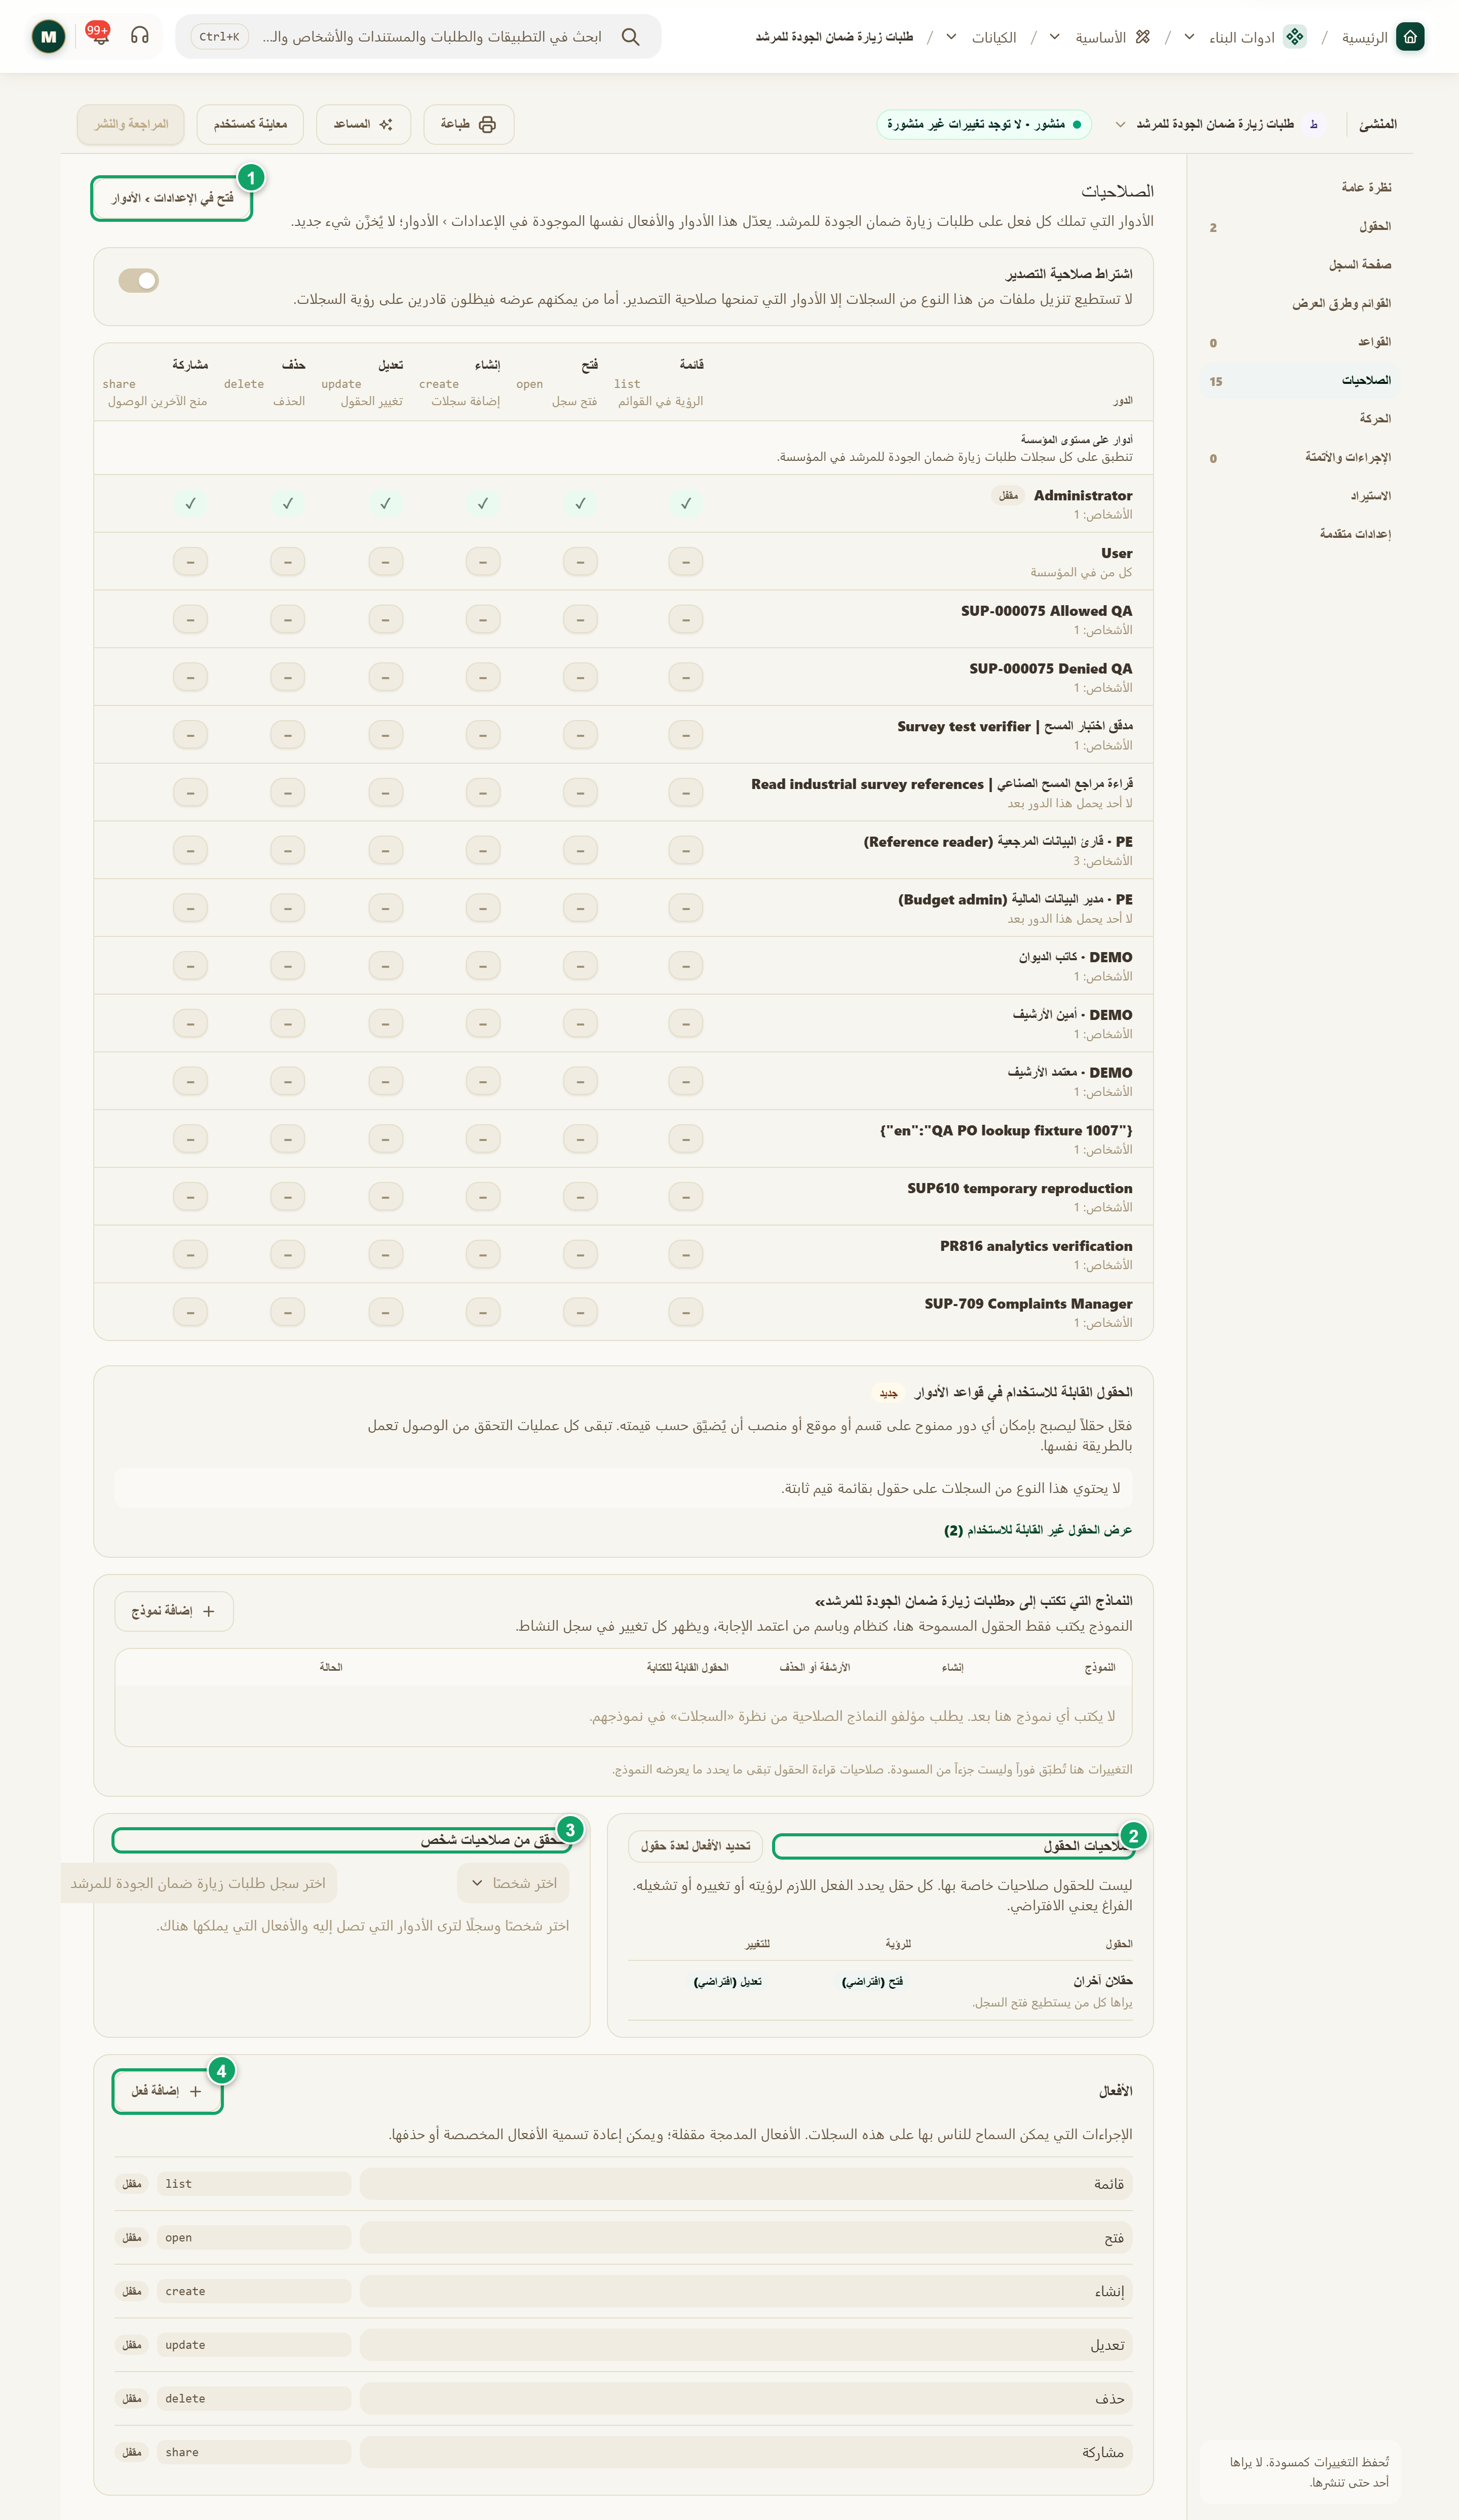
\includegraphics[width=0.95\linewidth,height=0.72\textheight,keepaspectratio]{figures/screens/ch06-ws-access-ar.png}
\caption{قسم «الصلاحيات»}
\label{fig:builder-access-screen}
\shotnote{يعرض القسم الأدوار والأفعال على هذا النوع، ثم صلاحيات الحقول وأداة فحص الوصول وقائمة الأفعال. والأدوار الظاهرة أدوار مؤسسة الاختبار. ① «فتح في الإعدادات › الأدوار»: يفتح الأدوار نفسها في الإعدادات. ② «صلاحيات الحقول»: تحدد الفعل اللازم لرؤية حقل أو تغييره. ③ «التحقق من صلاحيات شخص»: يبيّن ما يستطيعه شخص على سجل. ④ «إضافة فعل»: يضيف فعلاً مخصصاً مثل الاعتماد.}
\end{figure}


\begin{table}[H]
\centering
\caption{الأفعال المدمجة}
\label{tab:builder-access-verbs}
\begin{tabularx}{\linewidth}{R{3.6cm} Y}
\rcHeaderRow
\thh{الفعل} & \thh{ماذا يسمح به؟}\\
\en{list} & الرؤية في القوائم.\\
\en{open} & فتح سجل.\\
\en{create} & إضافة سجلات.\\
\en{update} & تغيير الحقول.\\
\en{delete} & الحذف.\\
\en{share} & منح الآخرين الوصول.\\
\en{export} & تنزيل ملف، ويظهر عند تفعيل «اشتراط صلاحية التصدير».\\
\end{tabularx}
\end{table}

\begin{table}[H]
\centering
\caption{ما الذي تجده هنا؟}
\label{tab:builder-access-data}
\begin{tabularx}{\linewidth}{R{3.6cm} Y}
\rcHeaderRow
\thh{البطاقة} & \thh{المحتوى والإجراء}\\
الأدوار والأفعال & اضغط الخانة لتمنح الدور فعلاً أو تسحبه. تظهر أدوار على مستوى المؤسسة، وأدوار على سجل واحد، وأدوار أخرى لها صلاحيات هنا.\\
صلاحيات الحقول & ليست للحقول صلاحيات خاصة؛ بل يحدد كل حقل الفعل اللازم «للرؤية» أو «للتغيير» أو «للتشغيل». الفراغ يعني الافتراضي.\\
الأفعال & «إضافة فعل» مخصص، مثل «اعتماد الميزانية»، ثم منحه للأدوار.\\
الحقول القابلة للاستخدام في قواعد الأدوار & تسمح بتضييق الدور حسب قيمة حقل، مثل الفرع.\\
النماذج التي تكتب إلى هذا النوع & تحدد النماذج المسموح لها بكتابة حقول هذا النوع. التغيير هنا يُطبّق فوراً، وليس جزءاً من المسودة.\\
التحقق من صلاحيات شخص & تختار شخصاً وسجلاً فترى الأدوار التي تصل إليه والأفعال التي يملكها.\\
\end{tabularx}
\end{table}

\begin{figure}[H]
\centering
\begin{tikzpicture}[node distance=0.5cm]
\node[entity] (role) {\RL{الدور}};
\node[entity,below=0.7cm of role] (verb) {\RL{الفعل}};
\node[entityOpt,below right=0.7cm and 0.3cm of verb] (field) {\RL{حقل يطلب الفعل}};
\node[entityOpt,below left=0.7cm and 0.3cm of verb] (records) {\RL{سجلات النوع}};
\draw[dependsOn] (role) -- (verb);
\draw[dependsOnOpt] (verb.south) -- ++(0,-0.3) -| (field.north);
\draw[dependsOnOpt] (verb.south) -- ++(0,-0.3) -| (records.north);
\end{tikzpicture}
\rclegend
\caption{من الدور إلى ما يستطيع الشخص فعله}
\label{fig:builder-access-model}
\shotnote{يوضّح الشكل أن الشخص لا يأخذ الصلاحية مباشرة، بل يأخذها من دوره، والدور يملك أفعالاً على سجلات النوع. ويمكن لحقل حساس أن يطلب فعلاً بعينه، فلا يراه أو يغيّره إلا من يملك ذلك الفعل. لذلك ابدأ بالأفعال المدمجة، ولا تضف فعلاً مخصصاً إلا لعمل له معنى مستقل مثل الاعتماد.}
\end{figure}

\subsection{خطوات العمل والتحقق}
\begin{enumerate}
\item افتح نوع السجلات واختر «الصلاحيات»، ثم راجع الأدوار الظاهرة.
\item اضغط الخانات لتمنح كل دور الأفعال التي يحتاجها عمله فقط.
\item للحقول الحساسة، افتح «صلاحيات الحقول» وحدد الفعل اللازم لرؤيتها أو تغييرها.
\item استخدم «التحقق من صلاحيات شخص» على موظف وسجل تجريبي، ثم انشر التغييرات.
\end{enumerate}

\textbf{تحقق ومعالجة المشكلة:} يجب أن تُظهر أداة التحقق الأفعال المتوقعة للشخص، وأن يرى المستخدم بعد النشر ما يخصه فقط. فإذا ظهرت رسالة «تحتاج فعل «تحديث» على الأدوار لتغيير الصلاحيات»، فاطلب ذلك من مسؤول المؤسسة؛ وإذا لم يظهر حقل لمستخدم، فراجع الفعل المطلوب له في «صلاحيات الحقول».

\clearpage
\section{الإجراءات والأتمتة}
\label{sec:builder-feature-actions}

الإجراء زر يظهر في السجل، يُنشئ مستند Word أو جدول بيانات من بيانات السجل، أو يفتح رابطاً، أو يبدأ مسار عمل. ويجمع هذا القسم أزرار النوع، ويعرض الأتمتة المرتبطة به، والحقول المحسوبة التي يعيد النظام حسابها دورياً.

\textbf{المسار ومن يستخدمه:} نوع السجلات ← «الإجراءات والأتمتة». يستخدمه من يبني النوع بعد تجهيز القالب أو مسار العمل الذي سيستدعيه الزر.

\begin{rcnote}[مثال: شركة الأفق]
يضيف مسؤول النظام إلى طلب الزيارة زراً من نوع «مستند Word» يُنشئ خطاب تأكيد الزيارة من بيانات الطلب، ويجعله متاحاً لمن يملك فعل الاعتماد فقط. ويبدأ الزر من ①.
\end{rcnote}

\begin{figure}[H]
\centering
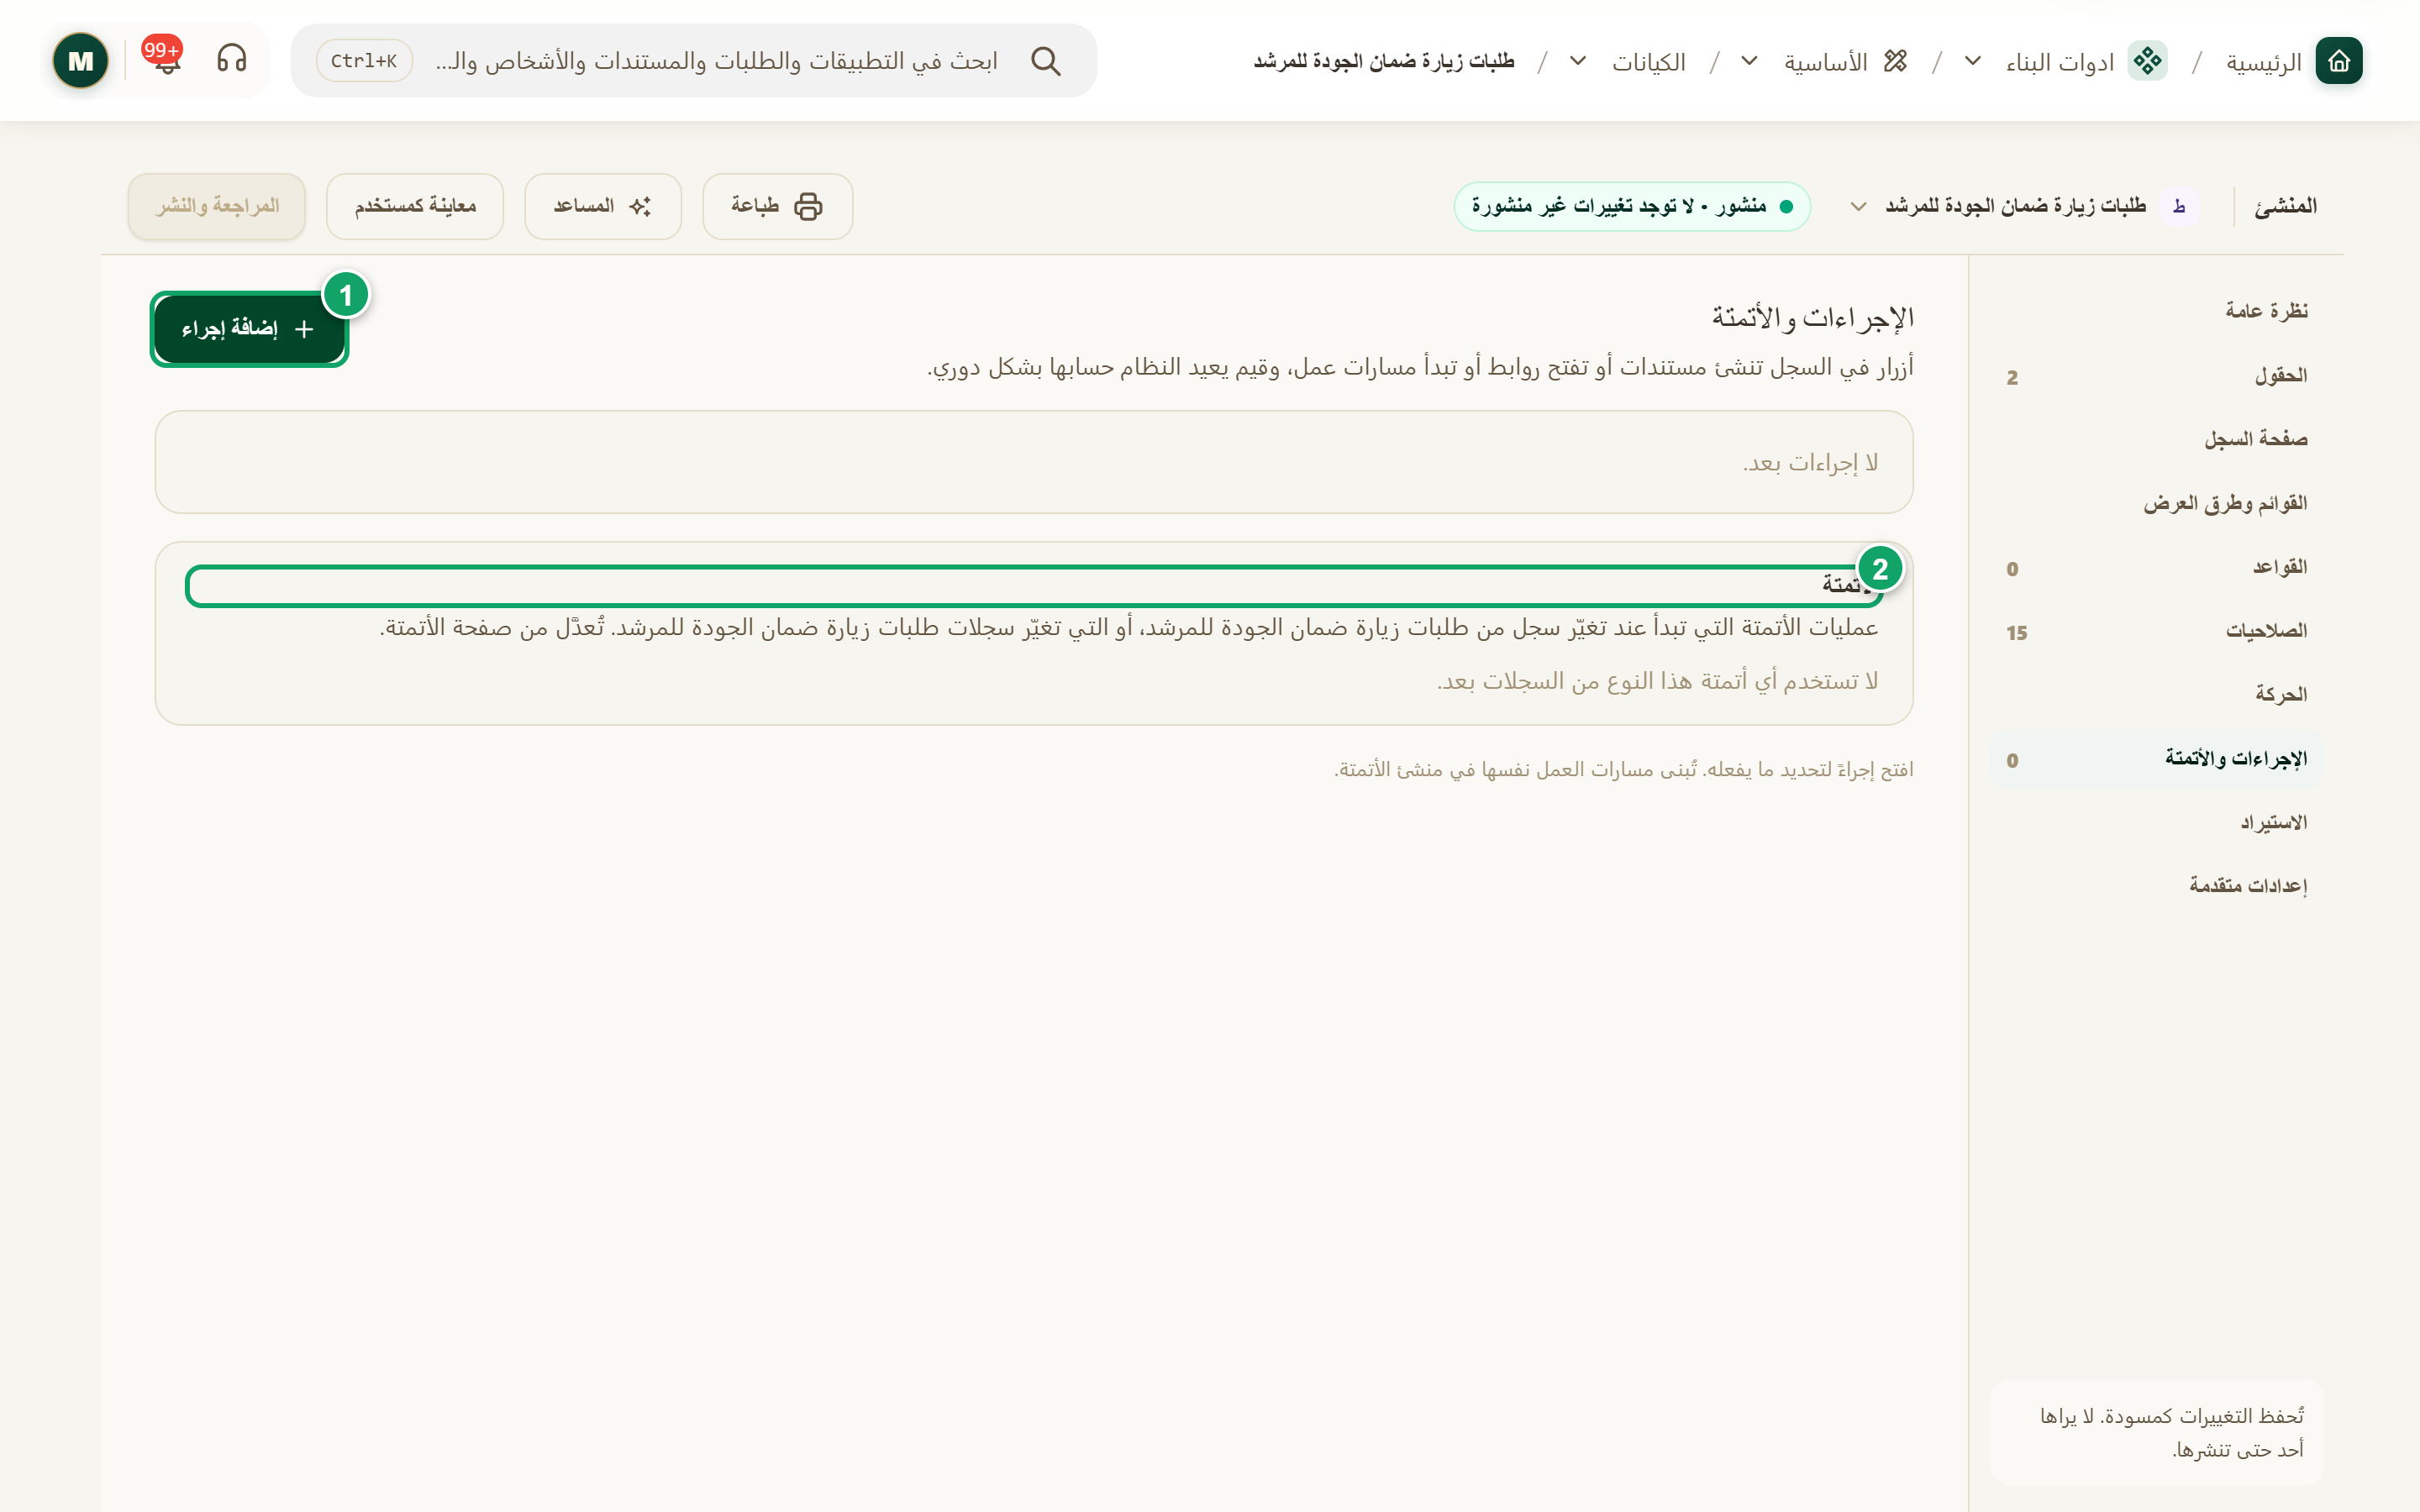
\includegraphics[width=0.95\linewidth,height=0.72\textheight,keepaspectratio]{figures/screens/ch06-ws-actions-ar.png}
\caption{قسم «الإجراءات والأتمتة»}
\label{fig:builder-actions-screen}
\shotnote{يعرض القسم أزرار النوع والأتمتة المرتبطة به، وهما فارغان في النوع الاختباري. ① «إضافة إجراء»: يُنشئ زراً جديداً ويفتحه لتحدد ما يفعله. ② «الأتمتة»: قائمة للاطلاع على الأتمتة التي تبدأ بتغيّر سجلات النوع أو تغيّرها.}
\end{figure}


\begin{table}[H]
\centering
\caption{ما الذي تجده هنا؟}
\label{tab:builder-actions-data}
\begin{tabularx}{\linewidth}{R{3.6cm} Y}
\rcHeaderRow
\thh{الجزء} & \thh{المحتوى والإجراء}\\
الإجراءات & لكل إجراء نوعه: «مستند Word» أو «جدول بيانات» أو «رابط» أو «مسار عمل»، ومن يستطيع تشغيله: «يتطلب» فعلاً معيناً، أو «كل من يستطيع تغيير السجل».\\
إضافة إجراء & يُنشئ «إجراء جديد» في المسودة ويفتحه في «الحقول»، حيث تختار ما يفعله والقالب أو المسار الذي يستخدمه.\\
الأتمتة & قائمة للاطلاع بالأتمتة التي «تبدأ عند التغيير» في سجل من هذا النوع، أو التي «تغيّر السجلات»، مع حالتها: «منشورة» أو «غير منشورة» أو «متوقفة مؤقتًا». تُعدَّل من صفحة الأتمتة.\\
يُعاد حسابه دوريًا & الحقول المحسوبة التي يعيد النظام حسابها «يوميًا» أو «أسبوعيًا» أو «شهريًا»، وتظهر عند وجودها فقط.\\
\end{tabularx}
\end{table}

\begin{figure}[H]
\centering
\begin{tikzpicture}[node distance=0.5cm]
\node[entity] (action) {\RL{زر الإجراء في السجل}};
\node[entityOpt,below right=0.7cm and 0.3cm of action] (tpl) {\RL{قالب مستند}};
\node[entityOpt,below left=0.7cm and 0.3cm of action] (sop) {\RL{مسار عمل}};
\draw[dependsOnOpt] (action.south) -- ++(0,-0.3) -| (tpl.north);
\draw[dependsOnOpt] (action.south) -- ++(0,-0.3) -| (sop.north);
\end{tikzpicture}
\rclegend
\caption{ما يستدعيه الإجراء}
\label{fig:builder-actions-model}
\shotnote{يوضّح الشكل أن الزر لا يعمل وحده، بل يستدعي شيئاً جاهزاً: قالب مستند تُعدّه في صفحات القوالب، أو مسار عمل تبنيه في الأتمتة. لذلك جهّز القالب أو المسار أولاً، ثم أنشئ الإجراء واربطه به.}
\end{figure}

\subsection{خطوات العمل والتحقق}
\begin{enumerate}
\item جهّز القالب أو مسار العمل الذي سيستدعيه الزر.
\item افتح نوع السجلات واختر «الإجراءات والأتمتة»، ثم اضغط «إضافة إجراء».
\item في الحقل الذي يُفتح، سمِّ الإجراء واختر نوعه والقالب أو المسار، ثم حدد الفعل اللازم لتشغيله.
\item انشر التغييرات، ثم افتح سجلاً تجريبياً واضغط الزر.
\end{enumerate}

\textbf{تحقق ومعالجة المشكلة:} يجب أن يظهر الزر في السجل لمن يملك الفعل المطلوب، وأن ينتج المستند أو يبدأ المسار. فإذا ظهر الإجراء بنوع «غير مضبوط»، فافتحه وأكمل اختيار ما يفعله؛ وإذا لم يظهر الزر لمستخدم، فراجع الفعل الذي يتطلبه.

\clearpage
\section{الحركة}
\label{sec:builder-feature-movement}

الحركة إعداد متخصص لسجلات تنقل مبلغاً أو كمية من سجل إلى آخر، مثل التحويل بين بنود الموازنة أو بين المستودعات. فكل سجل يحدد من أين يأتي المبلغ وإلى أين يذهب، ويحافظ كيان على تساوي الطرفين، ويرحّلهما معاً عندما يصل السجل إلى حالة تختارها. ولا تحتاج معظم أنواع السجلات إلى هذا القسم.

\textbf{المسار ومن يستخدمه:} نوع السجلات ← «الحركة». يستخدمه من يبني أنواع سجلات مالية أو مخزنية.

\begin{rcnote}[مثال: شركة الأفق]
لا يحتاج نوع «طلبات الزيارة» إلى الحركة. لكن لو أنشأت الأفق نوعاً لتحويل مبالغ بين بنود موازنة الفروع، فسيرحّل كل تحويل معتمد المبلغ من بند حلب إلى بند دمشق في خطوة واحدة. ولا يتجاوز مسؤول النظام شروط ② لأن نوع الطلبات لا يحتاج إليها.
\end{rcnote}

\begin{figure}[H]
\centering
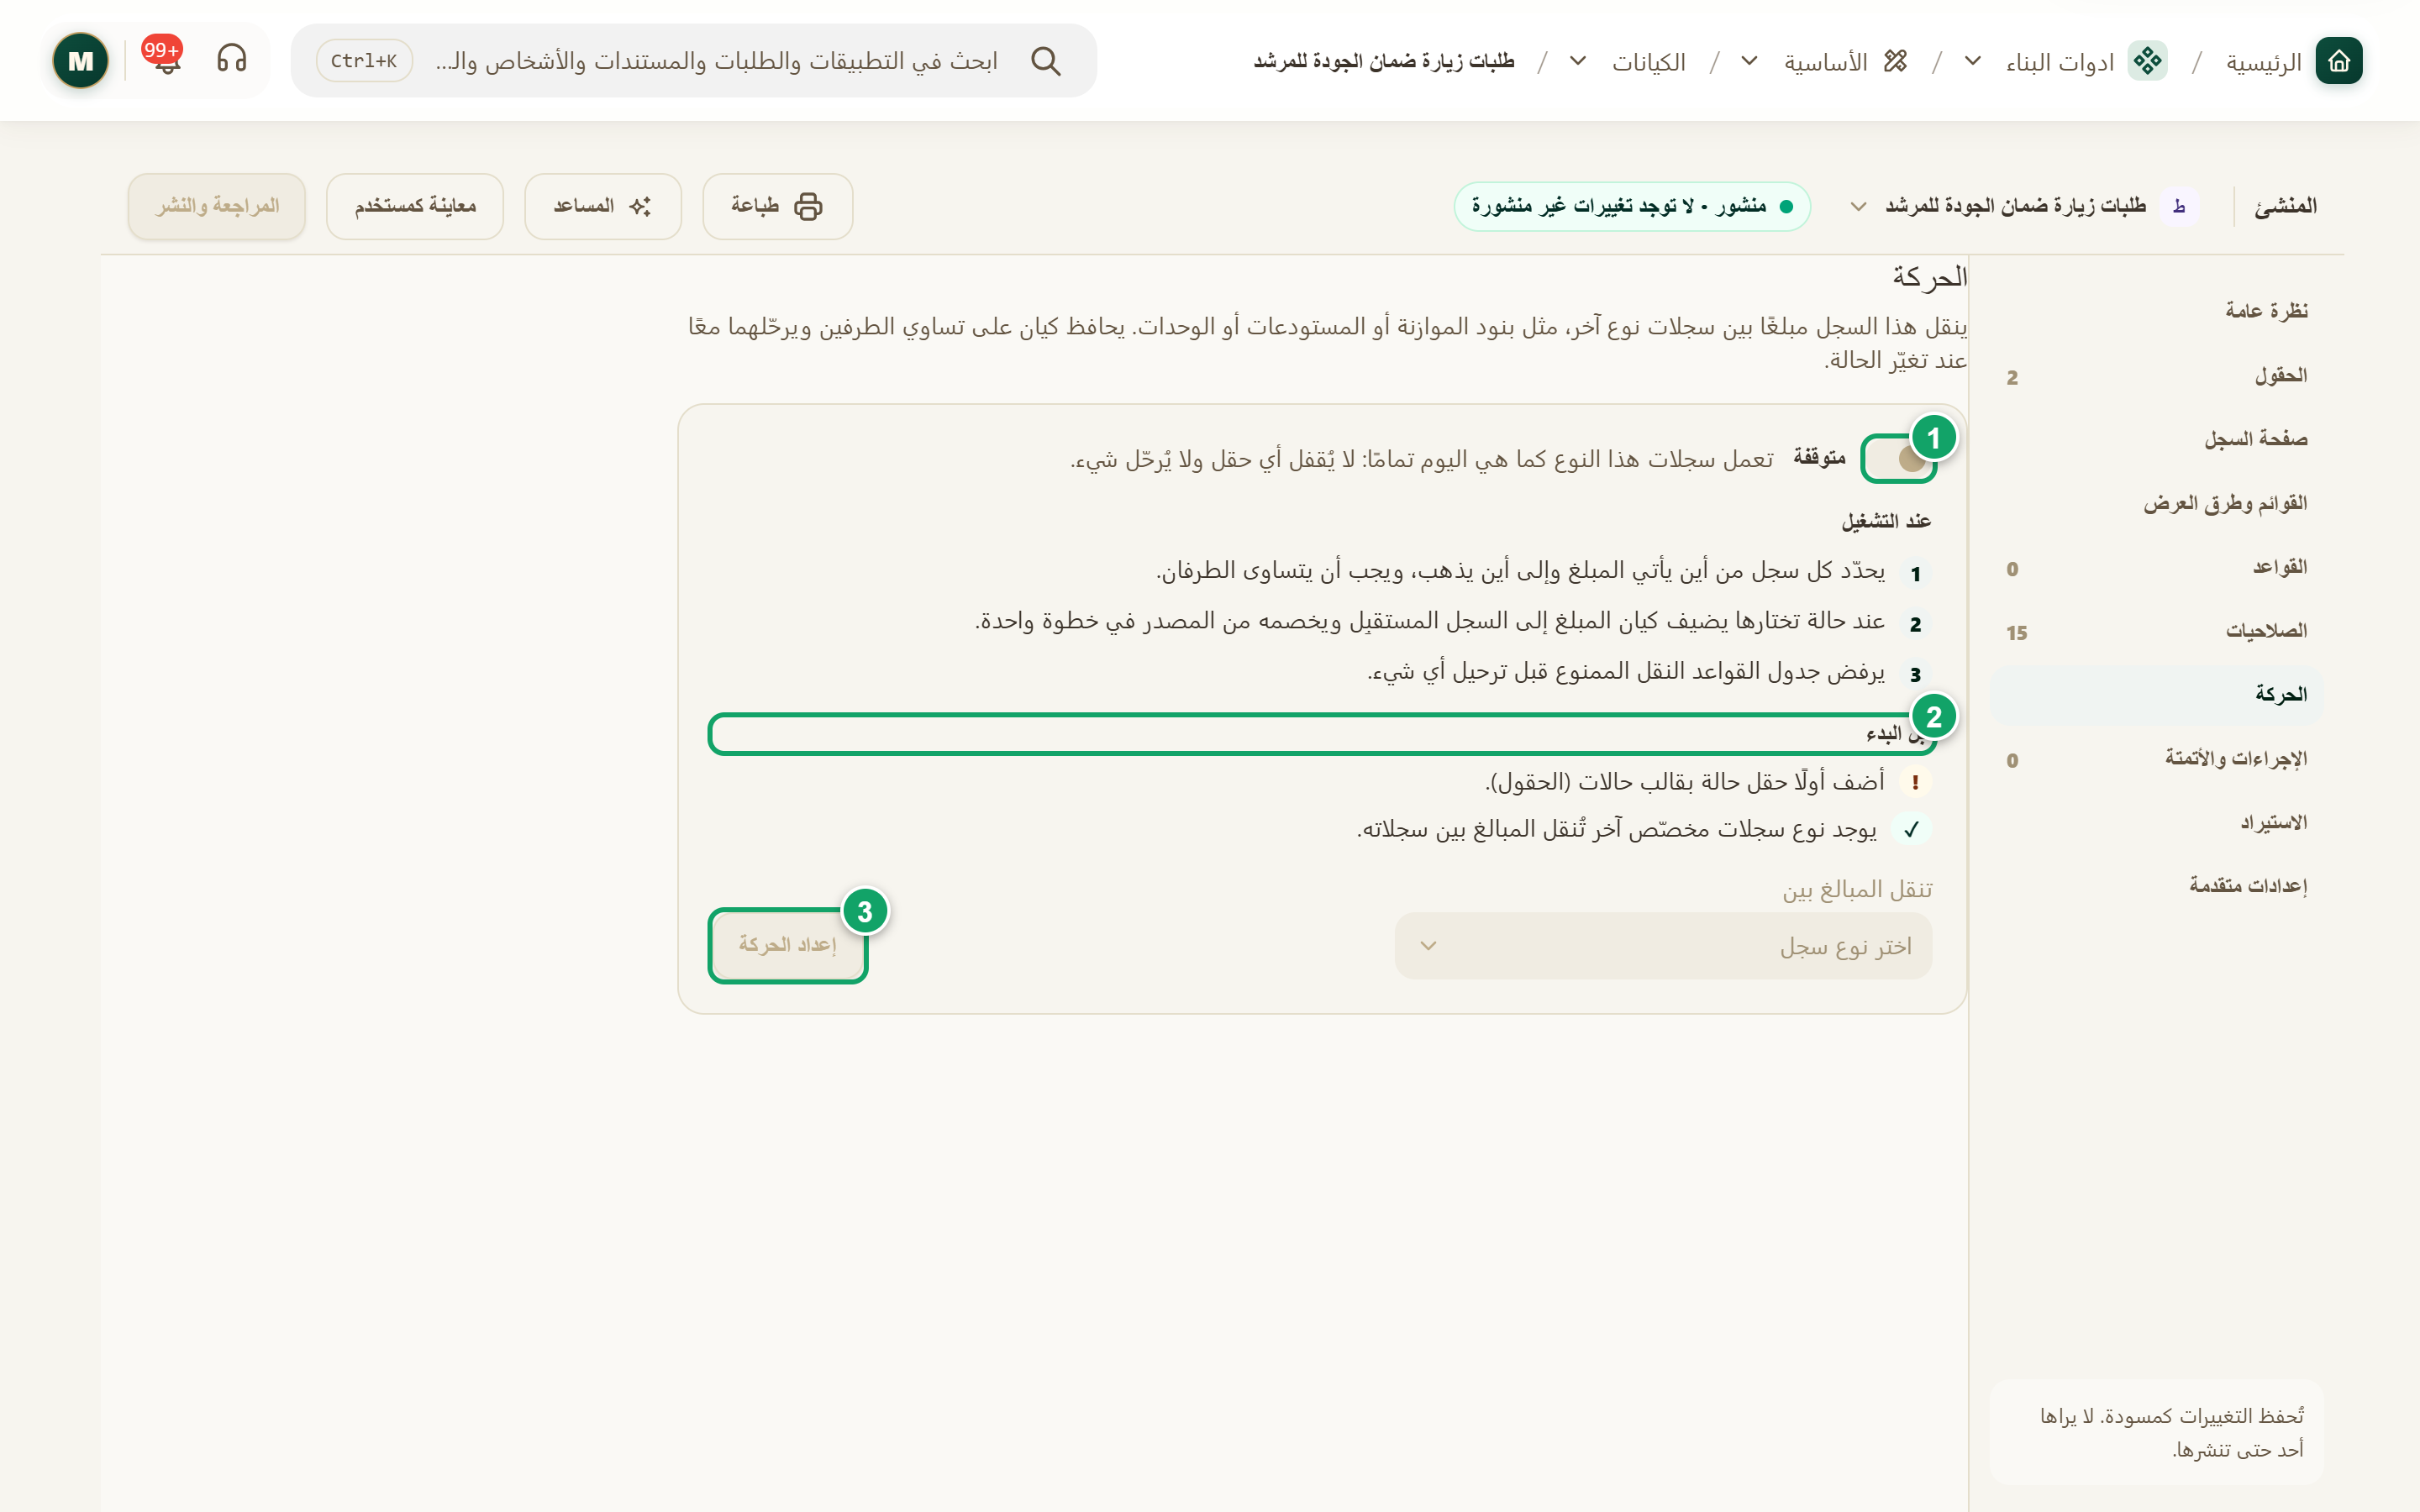
\includegraphics[width=0.95\linewidth,height=0.72\textheight,keepaspectratio]{figures/screens/ch06-ws-movement-ar.png}
\caption{قسم «الحركة» وهي متوقفة}
\label{fig:builder-movement-screen}
\shotnote{يشرح القسم ما تفعله الحركة عند تشغيلها، ويتحقق من شروطها قبل البدء. وتظهر علامة التنبيه لأن النوع الاختباري بلا حقل حالة. ① مفتاح التشغيل: متوقف، فلا يُرحَّل شيء. ② «قبل البدء»: الشروط الواجب توفرها، مع علامة لكل شرط. ③ «إعداد الحركة»: يبدأ الإعداد بعد اختيار النوع الذي تُنقل المبالغ بين سجلاته.}
\end{figure}


\begin{table}[H]
\centering
\caption{ما الذي تحتاجه وتضبطه؟}
\label{tab:builder-movement-data}
\begin{tabularx}{\linewidth}{R{3.6cm} Y}
\rcHeaderRow
\thh{الجزء} & \thh{المعنى}\\
قبل البدء & حقل «الحالة» بقالب حالات في هذا النوع، ونوع سجلات مخصّص آخر تُنقل المبالغ بين سجلاته، فيه حقلان رقميان لـ«الوارد» و«الصادر». ولا تعمل الحركة على الأنواع المدمجة.\\
الطرفان & من أين يأتي المبلغ وإلى أين يذهب، ويجب أن يتساويا.\\
الترحيل & الحالة التي يُرحَّل عندها المبلغ، وأثرها: حجز أو ترحيل أو فكّ الحجز أو عكس.\\
القواعد & ترفض النقل الممنوع قبل ترحيل أي شيء.\\
المجاميع الدورية وجرّب & تعرض المجاميع لكل فترة، وتختبر الإعداد قبل النشر.\\
\end{tabularx}
\end{table}

\begin{figure}[H]
\centering
\begin{tikzpicture}[node distance=0.5cm]
\node[stepBox] (a) {\RL{سجل الحركة: مسودة}};
\node[stepBox,below=of a] (b) {\RL{الوصول إلى حالة الترحيل}};
\node[stepBox,below=of b] (c) {\RL{خصم من المصدر وإضافة للمستقبِل}};
\draw[flowsTo] (a) -- (b);
\draw[flowsTo] (b) -- (c);
\end{tikzpicture}
\rclegend
\caption{متى يتحرك المبلغ؟}
\label{fig:builder-movement-flow}
\shotnote{يبيّن المخطط أن المبلغ لا يتحرك عند إنشاء السجل، بل عندما يصل إلى الحالة التي اخترتها للترحيل. وعندها يُخصم من المصدر ويُضاف إلى المستقبِل معاً، فلا يبقى طرف دون الآخر.}
\end{figure}

\subsection{خطوات العمل والتحقق}
\begin{enumerate}
\item تأكد من وجود حقل «الحالة» ونوع السجلات المستقبِل بحقلي الوارد والصادر.
\item افتح «الحركة»، واختر النوع من «تنقل المبالغ بين»، ثم اضغط «إعداد الحركة».
\item اضبط تبويبات «الطرفان» و«الترحيل» و«القواعد»، ثم استخدم «جرّب» قبل النشر.
\end{enumerate}

\textbf{تحقق ومعالجة المشكلة:} بعد النشر انقل سجلاً تجريبياً إلى حالة الترحيل، وتأكد من تغيّر رصيدي الطرفين بالمقدار نفسه. وإذا أوقفت الحركة لاحقاً، فتبقى المبالغ المرحّلة كما هي، ويتوقف ترحيل السجلات الجديدة فقط.

\clearpage
\section{الاستيراد}
\label{sec:builder-feature-import}

يحدد قسم «الاستيراد» كيف يحمّل الناس سجلات هذا النوع ويحدّثونها من ملفات Excel وCSV. وأهم ما فيه «مفاتيح الاستيراد»: حقل أو مجموعة حقول، مثل رمز أو رقم، يطابق بها كيان كل صف في الملف مع سجل موجود، فيحدّثه بدلاً من أن ينشئ نسخة مكررة. وعندما يكون الخيار متوقفاً، يعمل الاستيراد كالمعتاد ويخمّن المطابقة بالمعرّف أو الرمز أو الاسم.

\textbf{المسار ومن يستخدمه:} نوع السجلات ← «الاستيراد». يستخدمه من يبني نوع السجلات، قبل أن يبدأ الفريق تحديث السجلات من ملفات.

\begin{rcnote}[مثال: شركة الأفق]
يضيف مسؤول النظام مفتاح استيراد مبنياً على رقم الطلب \en{HZN-VR-0001}، فيرفع عمر حداد ملف Excel بمواعيد الزيارات المعدّلة، ويحدّث كيان الطلبات الموجودة نفسها دون إنشاء طلبات جديدة. ويضيف المفتاح من ② ثم يفحصه من ③.
\end{rcnote}

\begin{figure}[H]
\centering
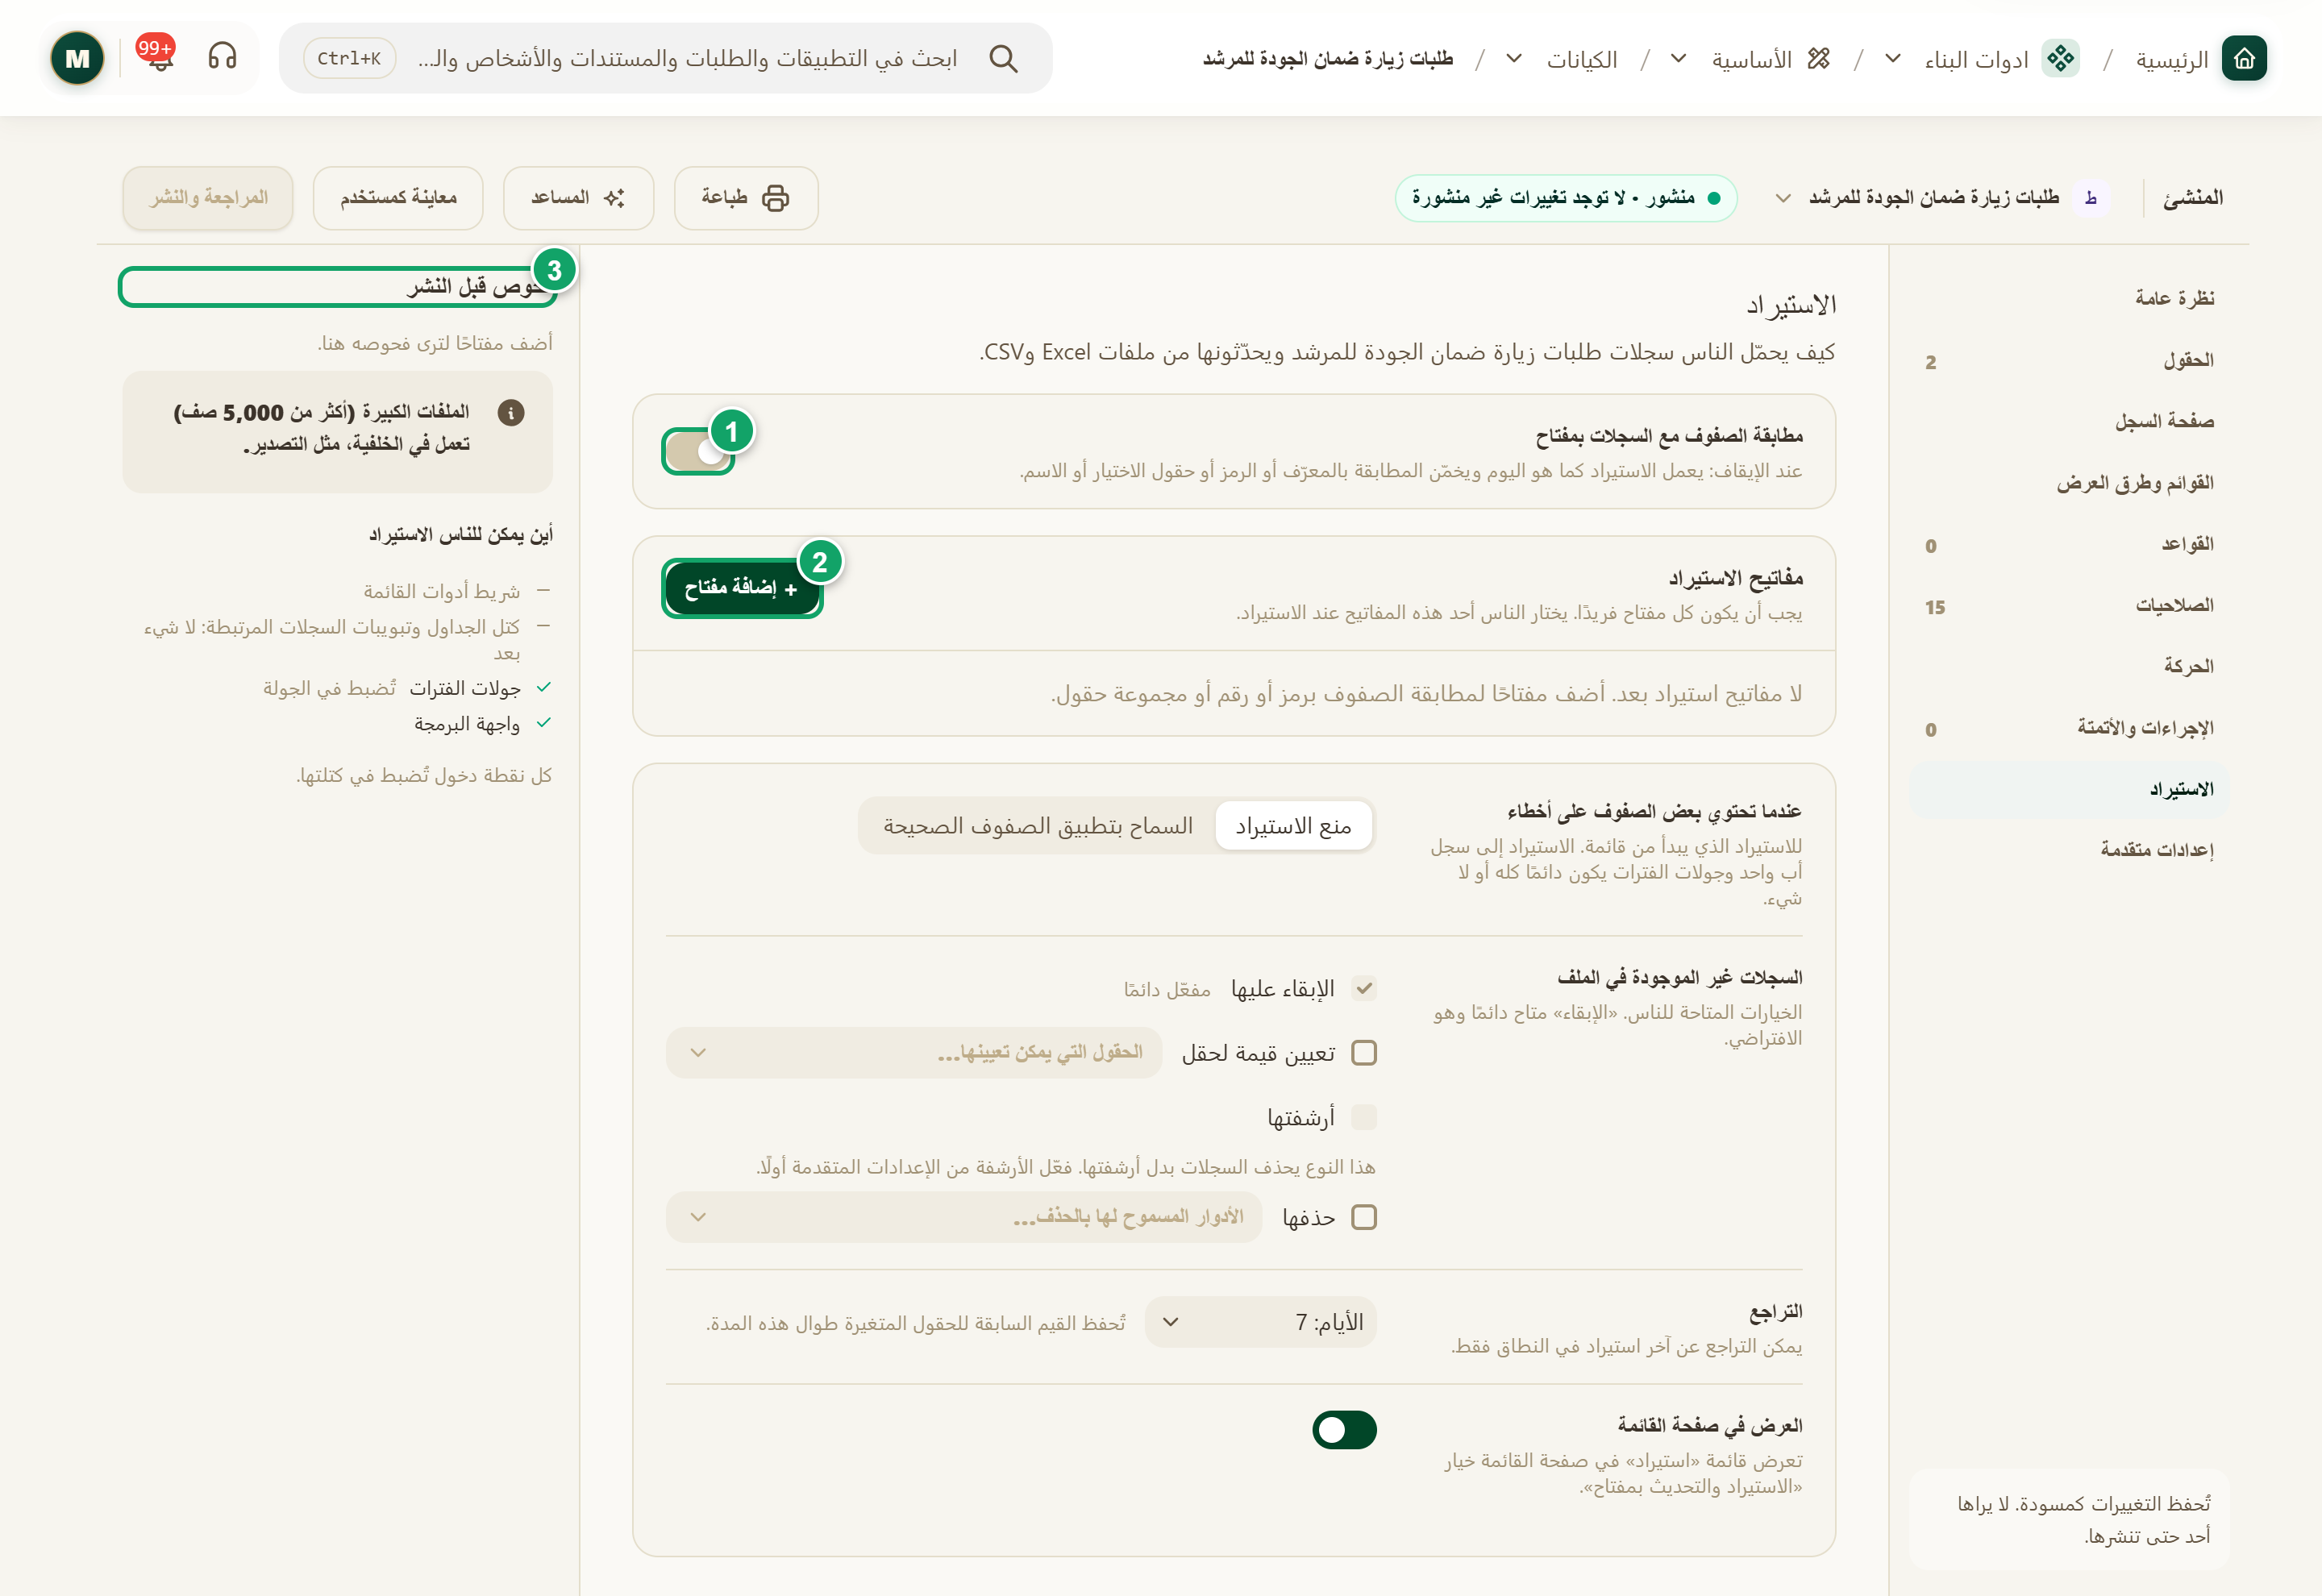
\includegraphics[width=0.95\linewidth,height=0.72\textheight,keepaspectratio]{figures/screens/ch06-ws-import-ar.png}
\caption{قسم «الاستيراد»}
\label{fig:builder-import-screen}
\shotnote{يحدد القسم طريقة تحديث السجلات من ملفات Excel وCSV، والمطابقة بالمفاتيح متوقفة هنا. ① مفتاح «مطابقة الصفوف مع السجلات بمفتاح». ② «+ إضافة مفتاح»: يضيف الحقل الذي تُطابق به الصفوف. ③ «فحوص قبل النشر»: تظهر فيها نتيجة «تشغيل الفحص» بعد إضافة مفتاح، لتتأكد من أنه فريد في السجلات المحفوظة.}
\end{figure}


\begin{table}[H]
\centering
\caption{ما الذي تجده هنا؟}
\label{tab:builder-import-data}
\begin{tabularx}{\linewidth}{R{3.6cm} Y}
\rcHeaderRow
\thh{الجزء} & \thh{المحتوى والإجراء}\\
مطابقة الصفوف مع السجلات بمفتاح & يفعّل الاستيراد بالمفاتيح. وعند الإيقاف يخمّن الاستيراد المطابقة كما في السابق.\\
مفاتيح الاستيراد & لكل مفتاح الحقول التي «يتكوّن من»ها، وأين يكون «فريد ضمن»ه، وطريقة «التوحيد» مثل تجاهل المسافات أو الأصفار البادئة، وهل هو «مدعوم بـ» قيمة فريدة، وحالته «جاهز» أو «مشكلة».\\
السلوك & ما يحدث «عندما تحتوي بعض الصفوف على أخطاء»: «منع الاستيراد» أو «السماح بتطبيق الصفوف الصحيحة»، وما يحدث لـ«السجلات غير الموجودة في الملف»: الإبقاء عليها أو أرشفتها أو حذفها، ومدة «التراجع» عن آخر استيراد.\\
فحوص قبل النشر & «تشغيل الفحص» يتأكد من أن المفتاح فريد في السجلات المحفوظة، ويعرض السجلات المتكررة أو الفارغة.\\
\end{tabularx}
\end{table}

\begin{figure}[H]
\centering
\begin{tikzpicture}[node distance=0.5cm]
\node[stepBox] (a) {\RL{إضافة مفتاح استيراد}};
\node[stepBox,below=of a] (b) {\RL{تشغيل الفحص}};
\node[stepBox,below=of b] (c) {\RL{ضبط السلوك}};
\node[stepBox,below=of c] (d) {\RL{النشر ثم استيراد ملف}};
\draw[flowsTo] (a) -- (b);
\draw[flowsTo] (b) -- (c);
\draw[flowsTo] (c) -- (d);
\end{tikzpicture}
\rclegend
\caption{تجهيز الاستيراد بالمفاتيح}
\label{fig:builder-import-flow}
\shotnote{يضع المخطط الفحص بعد إضافة المفتاح مباشرة، لأن المفتاح الذي تتكرر قيمته بين سجلين لا يعرف أيهما يحدّث. ثم تحدد ما يحدث للأخطاء والسجلات الغائبة عن الملف، لأن الاختيار الخاطئ هنا قد يؤرشف سجلات أو يحذفها. ولا يعمل شيء من ذلك قبل النشر.}
\end{figure}

\subsection{خطوات العمل والتحقق}
\begin{enumerate}
\item افتح نوع السجلات واختر «الاستيراد»، ثم فعّل «مطابقة الصفوف مع السجلات بمفتاح».
\item اضغط «+ إضافة مفتاح»، واختر الحقل الذي يميّز كل سجل، مثل الرمز أو الرقم التسلسلي.
\item اضغط «تشغيل الفحص»، وعالج أي سجلات متكررة أو فارغة يظهرها.
\item اختر السلوك المناسب للأخطاء والسجلات الغائبة، ثم انشر التغييرات.
\end{enumerate}

\textbf{تحقق ومعالجة المشكلة:} يجب أن تظهر حالة المفتاح «جاهز» وأن يظهر في الفحص أنه فريد. فإذا ظهر أن بعض السجلات ستتشارك المفتاح نفسه، فصحّح قيمها أولاً. ولا تختر حذف السجلات الغائبة عن الملف إلا عن قصد، واستخدم «التراجع» إذا أخطأ استيراد.

\clearpage
\section{إعدادات متقدمة}
\label{sec:builder-feature-advanced}

تضم «إعدادات متقدمة» إعدادات نادراً ما تتغير بعد البداية، مثل اسم السجل في القوائم، ومنع التكرار، والتسلسل بين السجلات، والتطبيق الذي يظهر فيه النوع. وهي جزء من المسودة مثل بقية الأقسام، فلا تصل إلى الفريق قبل النشر.

\textbf{المسار ومن يستخدمه:} نوع السجلات ← «إعدادات متقدمة». يستخدمه من يبني النوع، غالباً عند إنشائه ثم عند الحاجة فقط.

\begin{rcnote}[مثال: شركة الأفق]
يجعل مسؤول النظام «اسم السجل» في طلبات الزيارة هو الرقم التسلسلي مع اسم الفرع، ويضع النوع في تطبيق «خدمات الفروع»، ويختار «أرشفة السجلات بدل حذفها» حتى لا يضيع أي طلب. وتطابق اختياراته الرقمين ① و④.
\end{rcnote}

\begin{figure}[H]
\centering
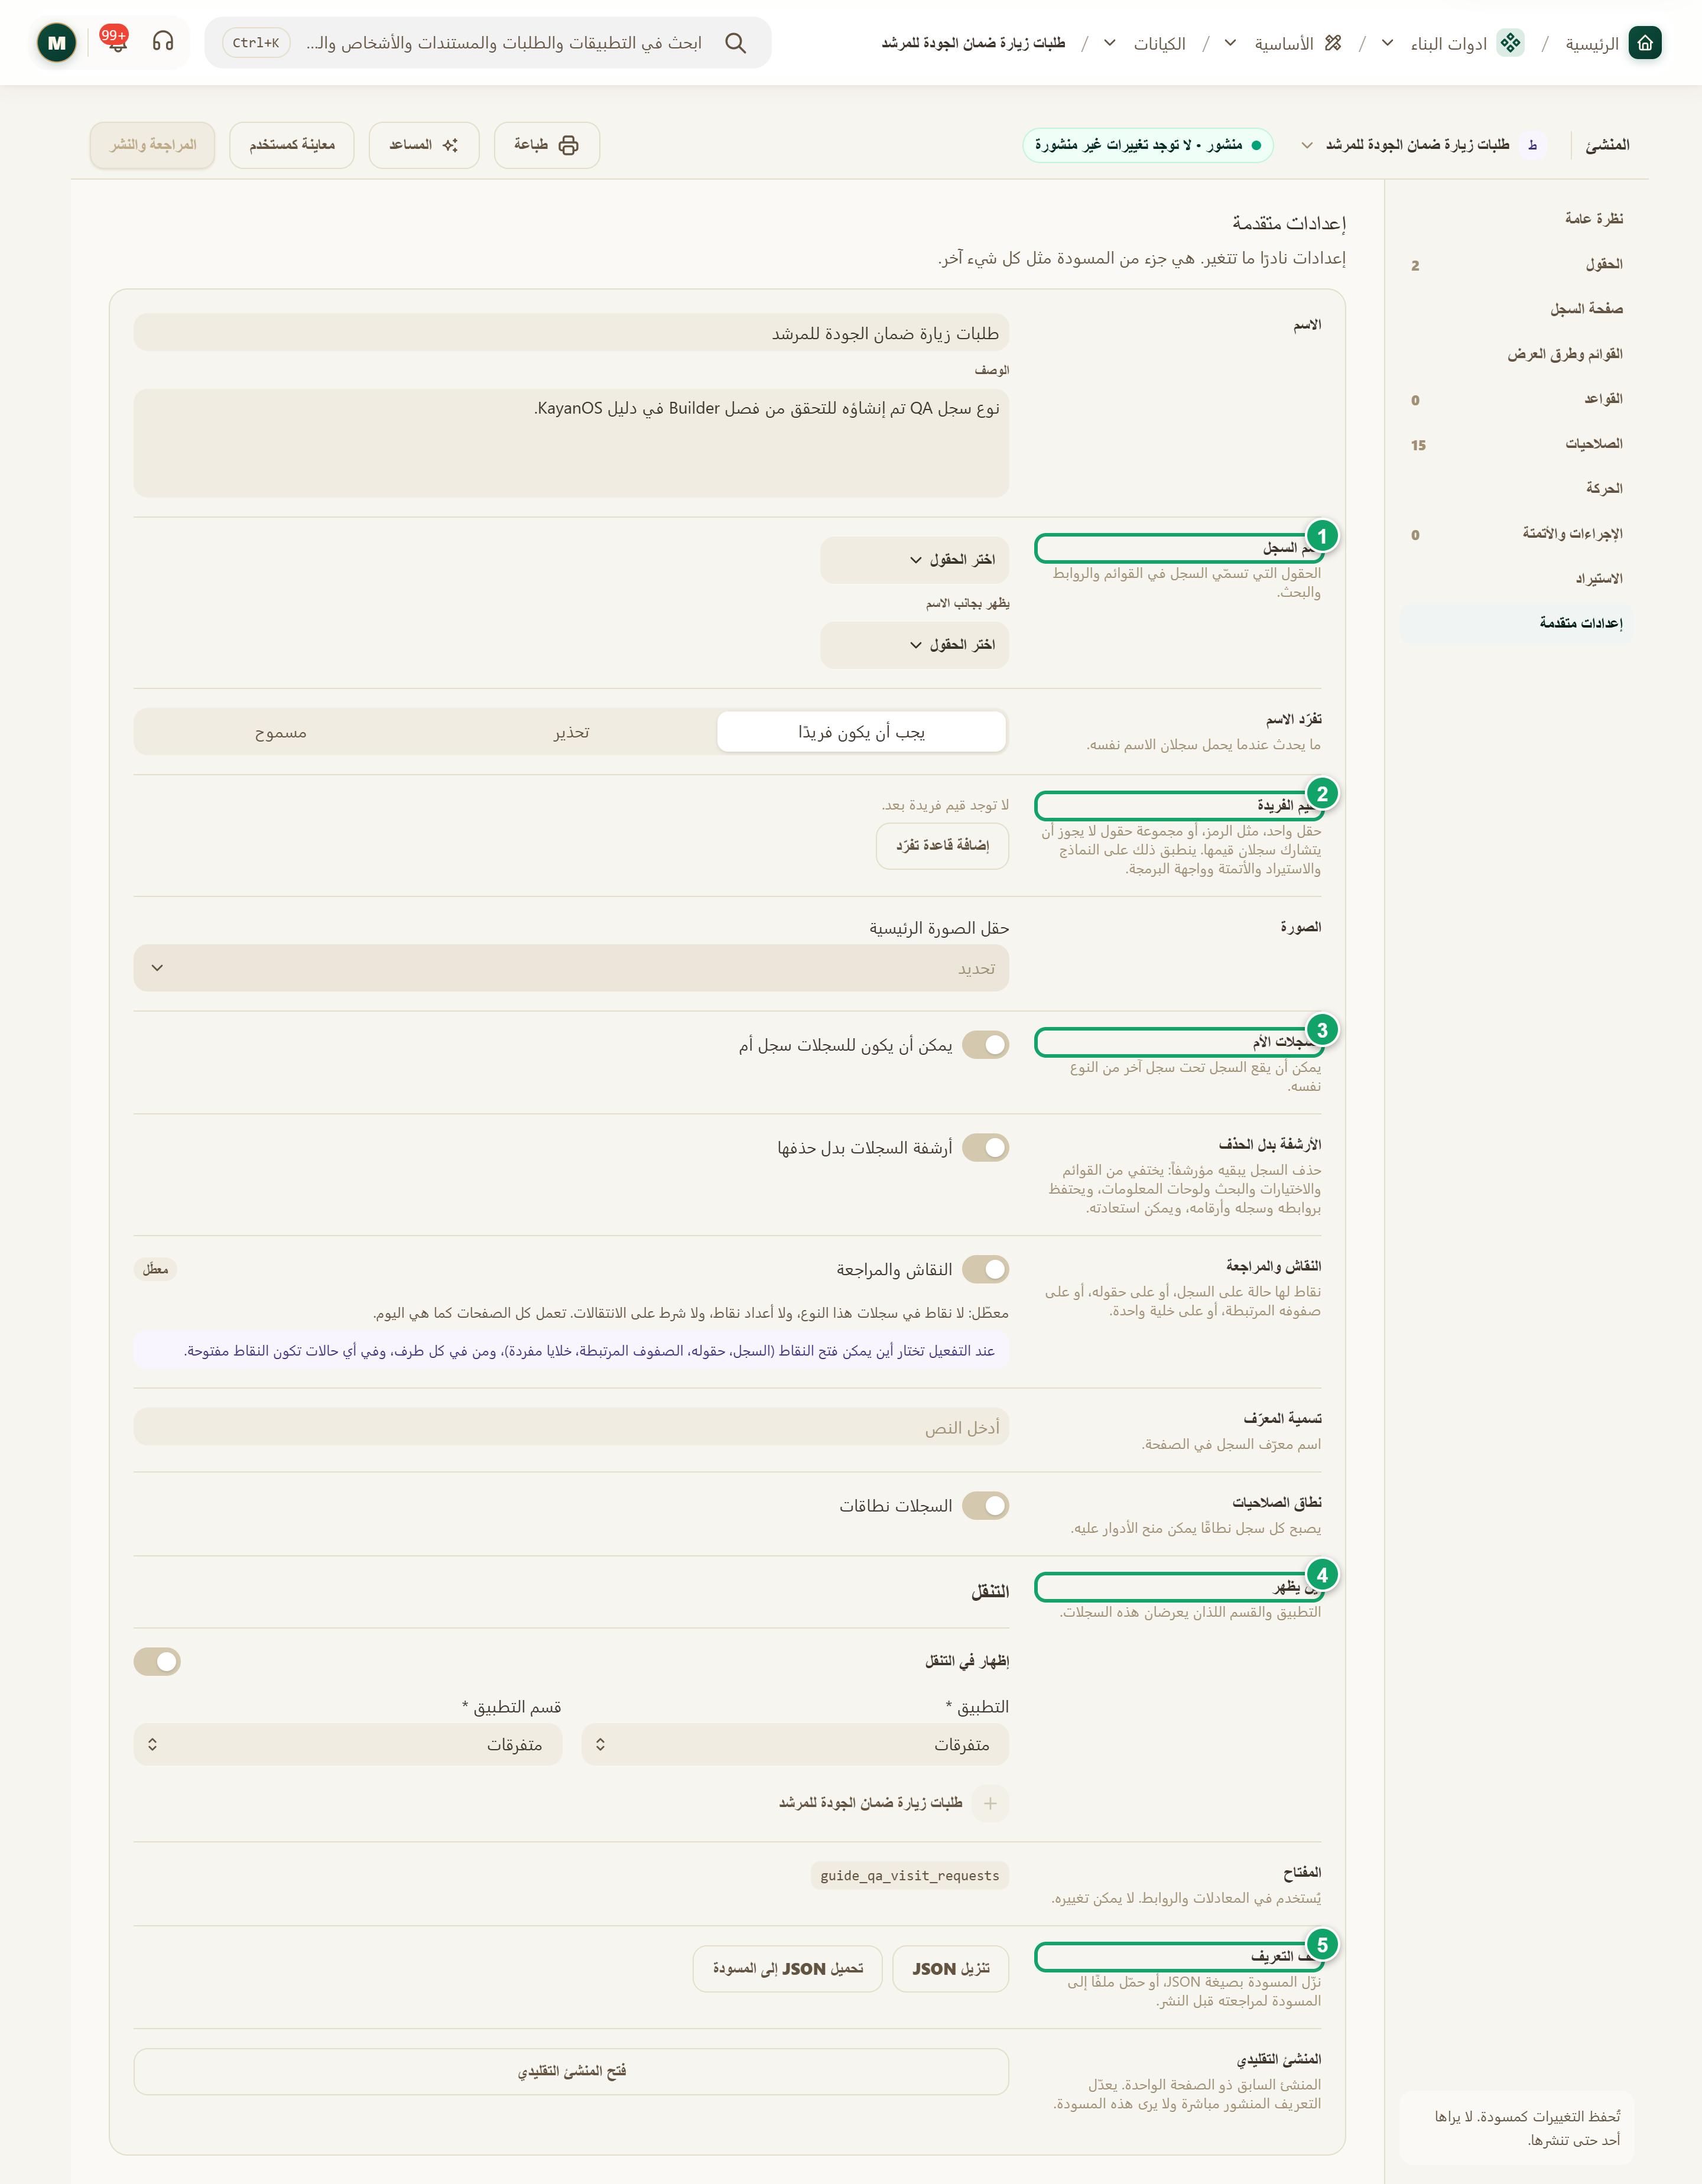
\includegraphics[width=0.95\linewidth,height=0.72\textheight,keepaspectratio]{figures/screens/ch06-ws-advanced-ar.png}
\caption{قسم «إعدادات متقدمة»}
\label{fig:builder-advanced-screen}
\shotnote{يجمع القسم إعدادات نادراً ما تتغير، ويظهر هنا لنوع السجلات الاختباري. ① «اسم السجل»: الحقول التي تسمّي السجل. ② «القيم الفريدة»: تمنع تكرار رمز أو مجموعة قيم. ③ «السجلات الأم»: تسمح بتسلسل أب وأبناء. ④ «أين يظهر»: التطبيق والقسم. ⑤ «ملف التعريف»: تنزيل الإعداد أو تحميله بصيغة JSON.}
\end{figure}


\begin{table}[H]
\centering
\caption{ما الذي تجده هنا؟}
\label{tab:builder-advanced-data}
\begin{tabularx}{\linewidth}{R{3.6cm} Y}
\rcHeaderRow
\thh{الإعداد} & \thh{المعنى}\\
اسم السجل & الحقول التي تسمّي السجل في القوائم والروابط والبحث، وحقل اختياري «يظهر بجانب الاسم».\\
تفرّد الاسم & ما يحدث عندما يحمل سجلان الاسم نفسه: «يجب أن يكون فريدًا» أو «تحذير» أو «مسموح».\\
القيم الفريدة & حقل، مثل الرمز، أو مجموعة حقول لا يجوز أن يتشارك سجلان قيمها، في النماذج والاستيراد والأتمتة أيضاً.\\
الصورة & الحقل الذي يُستخدم صورةً رئيسية للسجل.\\
السجلات الأم & تسمح بأن يقع السجل تحت سجل آخر من النوع نفسه، فتظهر طريقة العرض «شجرة».\\
الأرشفة بدل الحذف & تُخفي السجل المحذوف في الأرشيف بدلاً من حذفه نهائياً.\\
تسمية المعرّف & اسم معرّف السجل في الصفحة.\\
نطاق الصلاحيات & يجعل كل سجل نطاقاً يمكن منح الأدوار عليه، مثل منح مدير فرع صلاحية على فرعه فقط.\\
أين يظهر & «التطبيق» و«قسم التطبيق» اللذان يعرضان السجلات، و«إظهار في التنقل»، والأيقونة.\\
المفتاح & يُستخدم في المعادلات والروابط، ولا يمكن تغييره.\\
ملف التعريف & «تنزيل JSON» لنسخة من المسودة، أو «تحميل JSON إلى المسودة» لمراجعته قبل النشر.\\
المنشئ التقليدي & المنشئ السابق ذو الصفحة الواحدة؛ يعدّل التعريف المنشور مباشرة ولا يرى المسودة، فاستخدمه بحذر.\\
\end{tabularx}
\end{table}

\begin{figure}[H]
\centering
\begin{tikzpicture}[node distance=0.5cm]
\node[entity] (adv) {\RL{إعدادات متقدمة}};
\node[entityOpt,below right=0.7cm and 0.3cm of adv] (tree) {\RL{السجلات الأم}};
\node[entityOpt,below left=0.7cm and 0.3cm of adv] (scope) {\RL{نطاق الصلاحيات}};
\node[entityOpt,below=0.7cm of tree] (treeview) {\RL{عرض الشجرة}};
\node[entityOpt,below=0.7cm of scope] (roles) {\RL{أدوار على سجل واحد}};
\draw[dependsOnOpt] (adv.south) -- ++(0,-0.3) -| (tree.north);
\draw[dependsOnOpt] (adv.south) -- ++(0,-0.3) -| (scope.north);
\draw[dependsOnOpt] (tree) -- (treeview);
\draw[dependsOnOpt] (scope) -- (roles);
\end{tikzpicture}
\rclegend
\caption{إعدادان يفتحان إمكانات أخرى}
\label{fig:builder-advanced-effects}
\shotnote{يوضّح الشكل أن بعض الإعدادات المتقدمة شرط لإمكانات في أقسام أخرى: فتفعيل «السجلات الأم» يتيح عرض «شجرة» في القوائم، وتفعيل «نطاق الصلاحيات» يتيح منح أدوار على سجل واحد. لذلك إذا لم تجد إحدى هذه الإمكانات، فابدأ بمراجعة هذا القسم.}
\end{figure}

\subsection{خطوات العمل والتحقق}
\begin{enumerate}
\item افتح نوع السجلات واختر «إعدادات متقدمة».
\item اختر «اسم السجل» من حقول تميّز السجل فعلاً، مثل الرقم التسلسلي.
\item أضف «قاعدة تفرّد» للحقول التي يجب ألا تتكرر، وراجع التحذير إن وُجدت تكرارات حالية.
\item راجع «أين يظهر» لتتأكد من التطبيق والقسم، ثم انشر التغييرات.
\end{enumerate}

\textbf{تحقق ومعالجة المشكلة:} بعد النشر يجب أن تظهر السجلات في القوائم والبحث بالاسم الذي اخترته، وأن يُرفض إدخال قيمة فريدة مكررة. وقبل أي تعديل كبير، استخدم «تنزيل JSON» لتحتفظ بنسخة من الإعداد.

\clearpage
\section{المراجعة والنشر}
\label{sec:builder-feature-publish}

يحفظ «المنشئ» كل تعديل تجريه مسودةً، ولا يرى أحد غيرك هذه التغييرات حتى تنشرها. وتعرض «المراجعة والنشر» التغييرات كلها قبل النشر، وتمنعه إذا بقيت مشكلة يجب حلها. وكل نشر يُنشئ إصداراً جديداً يمكنك الرجوع إليه لاحقاً.

\textbf{المسار ومن يستخدمه:} نوع السجلات ← «المراجعة والنشر». يستخدمه من يبني النوع بعد أن ينهي مجموعة من التعديلات.

\begin{rcnote}[مثال: شركة الأفق]
قبل إطلاق «طلبات الزيارة» يستخدم مسؤول النظام «معاينة كمستخدم» ليرى الصفحة كما يراها عمر حداد، ثم ينشر الإصدار الأول، ويطلب من عمر تجربة طلب لزيارة فرع حلب. ويستخدم ③ قبل أن ينشر من ④.
\end{rcnote}

\begin{figure}[H]
\centering
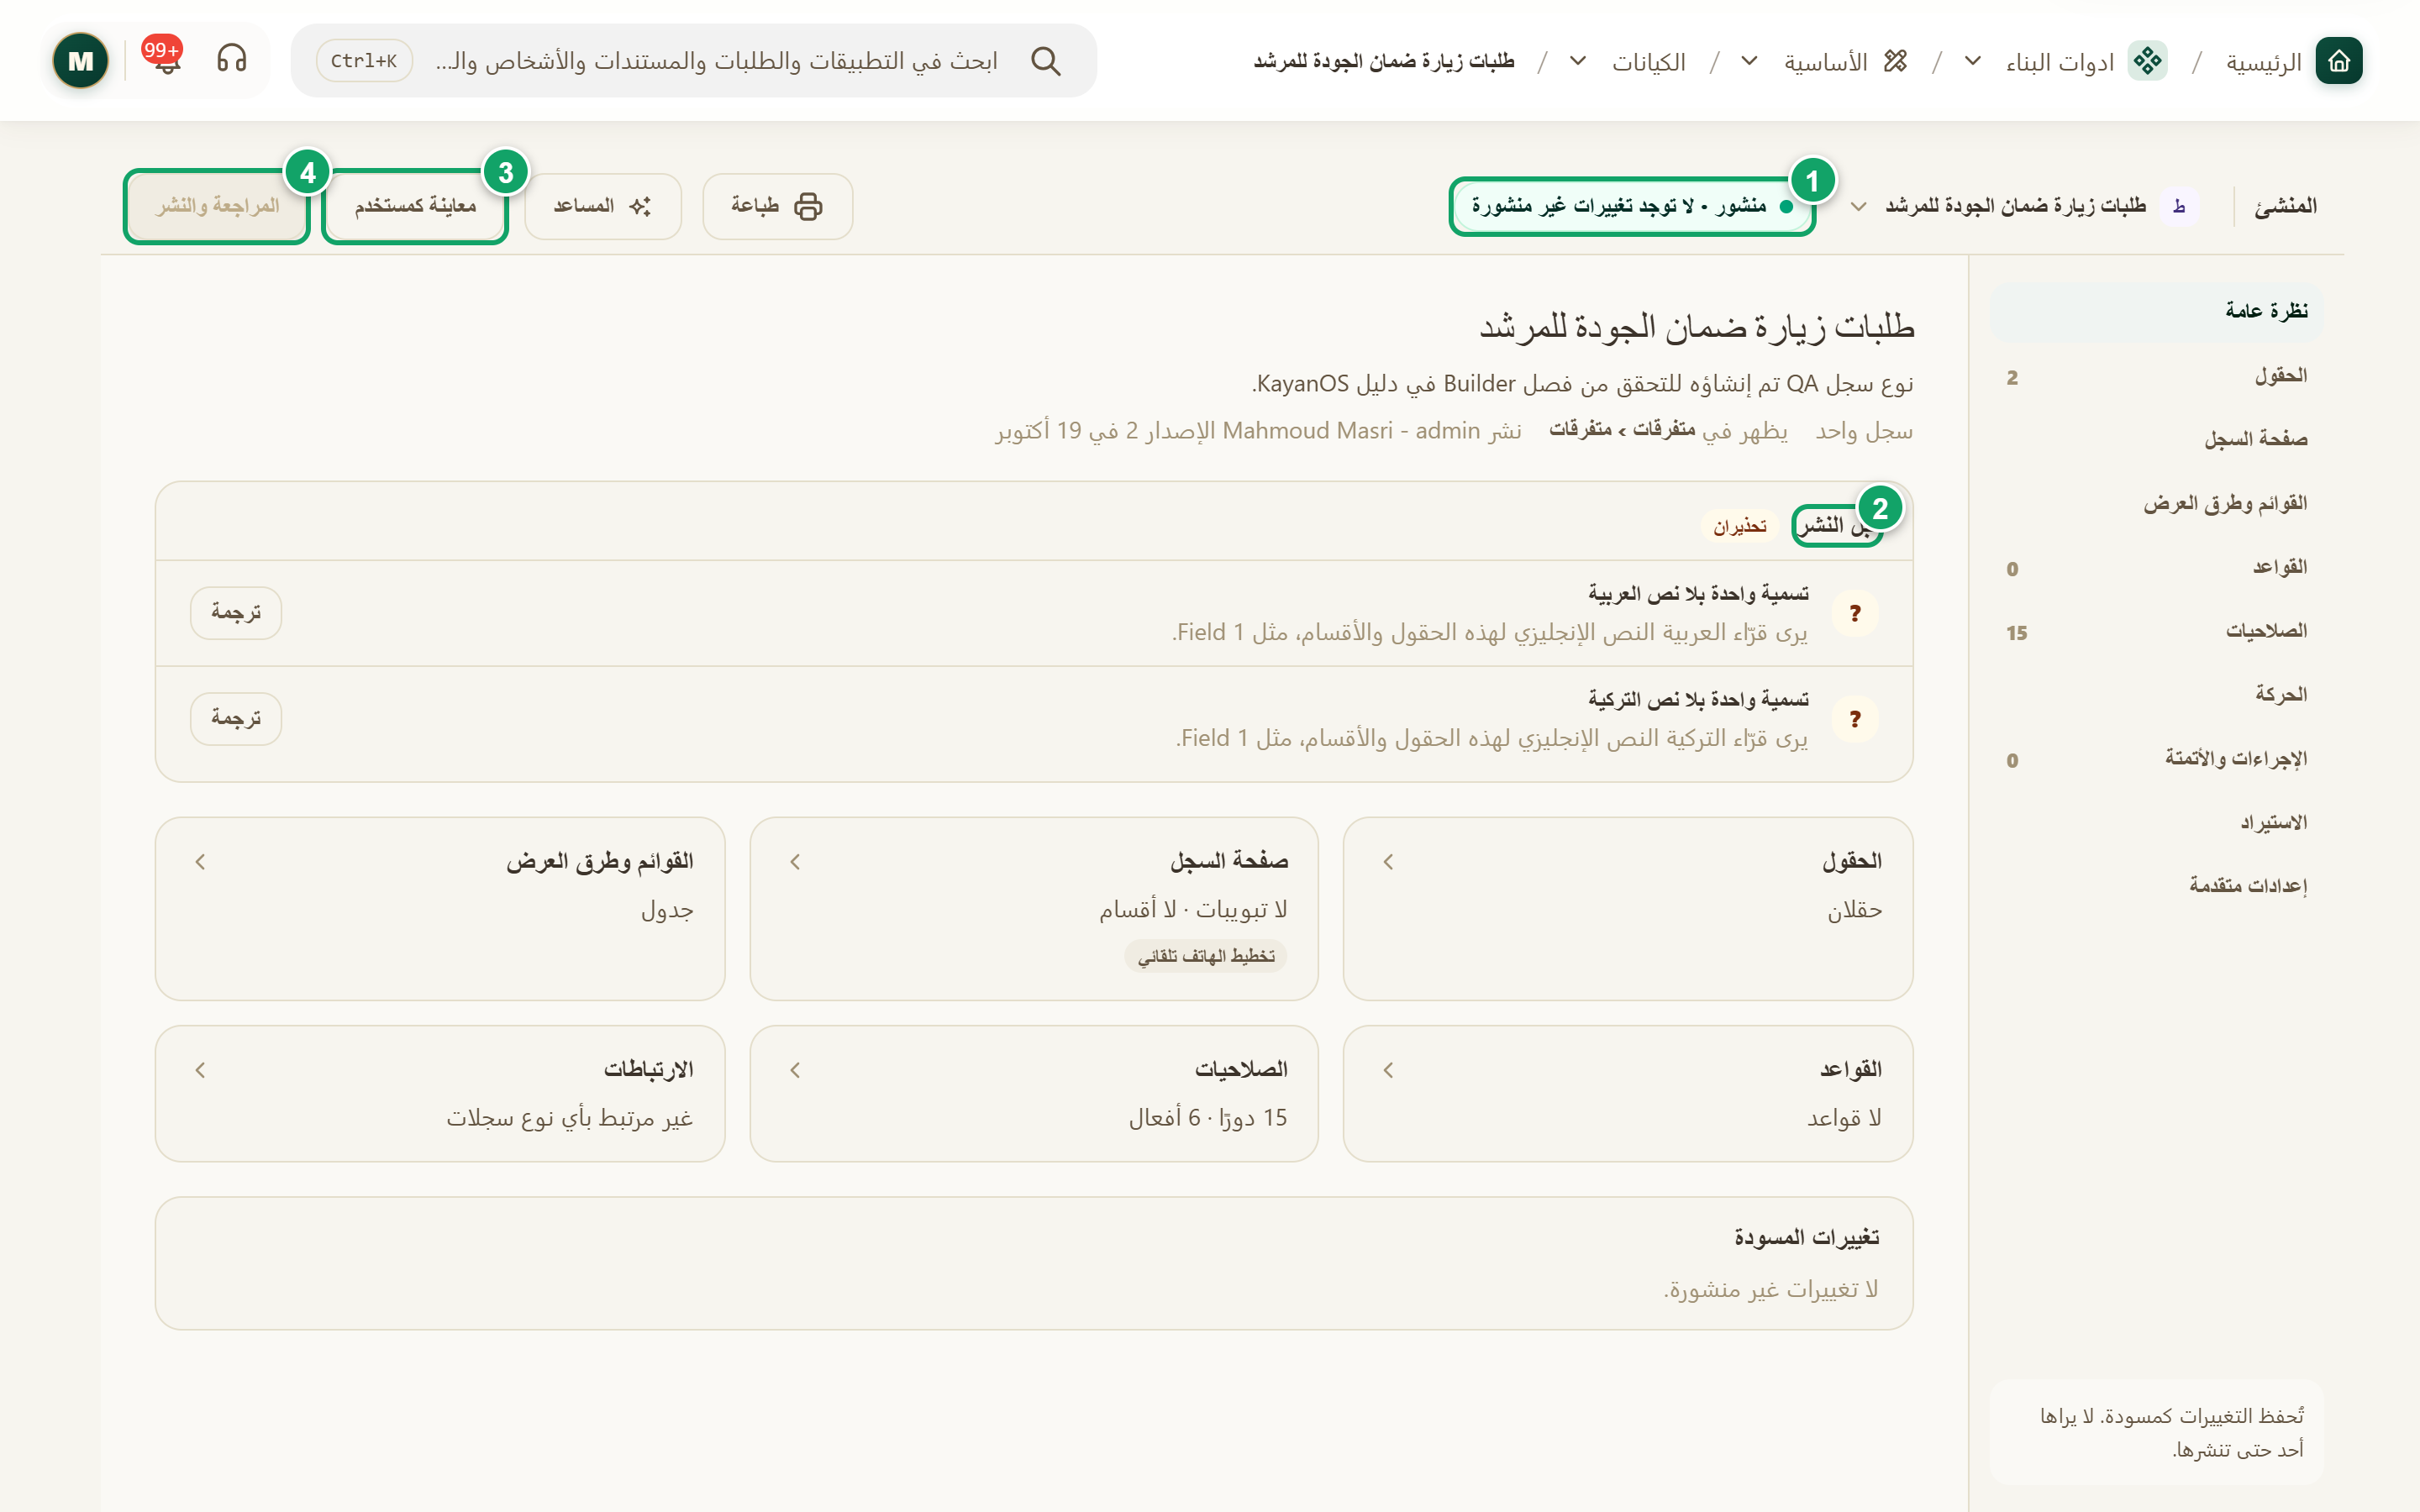
\includegraphics[width=0.95\linewidth,height=0.72\textheight,keepaspectratio]{figures/screens/ch06-ws-overview-ar.png}
\caption{«نظرة عامة» بعد النشر}
\label{fig:builder-publish-screen}
\shotnote{تلخّص «نظرة عامة» حالة النوع وما يجب إصلاحه قبل النشر. والنوع الاختباري هنا منشور في الإصدار 2 بعد اختبار هذا الفصل، وتبقى تحذيرات ترجمة لا تمنع النشر. ① الحالة: «منشور · لا توجد تغييرات غير منشورة». ② «قبل النشر»: المشكلات والتحذيرات. ③ «معاينة كمستخدم»: تجربة النوع كما يراه المستخدم. ④ «المراجعة والنشر»: يفتح قائمة التغييرات وزر النشر.}
\end{figure}


\begin{table}[H]
\centering
\caption{ما الذي تجده هنا؟}
\label{tab:builder-publish-data}
\begin{tabularx}{\linewidth}{R{3.6cm} Y}
\rcHeaderRow
\thh{العنصر} & \thh{المعنى والإجراء}\\
مسودة & حالة النوع وفيه تغييرات لم تُنشر. أما «منشور · لا توجد تغييرات غير منشورة» فيعني أن ما يراه الفريق هو آخر ما بنيته.\\
نظرة عامة & ملخص الحقول والصفحة والقوائم والقواعد، و«قبل أن تنشر» تعرض المشكلات التي تمنع النشر والتحذيرات.\\
معاينة كمستخدم & تعرض النوع كما سيراه المستخدم قبل النشر.\\
المراجعة والنشر & تعرض «مراجعة التغييرات» لكل تغيير، ثم تنشرها معاً بزر النشر.\\
سجل الإصدارات & يعرض الإصدارات السابقة، ويتيح «استعادة» إصدار منها.\\
تجاهل المسودة & يحذف التغييرات غير المنشورة ويعيد النوع إلى آخر إصدار منشور.\\
\end{tabularx}
\end{table}

\begin{figure}[H]
\centering
\begin{tikzpicture}[node distance=0.5cm]
\node[stepBox] (a) {\RL{تعديلات تُحفظ مسودة}};
\node[stepBox,below=of a] (b) {\RL{حل مشكلات «قبل أن تنشر»}};
\node[stepBox,below=of b] (c) {\RL{معاينة كمستخدم}};
\node[stepBox,below=of c] (d) {\RL{النشر: إصدار جديد}};
\draw[flowsTo] (a) -- (b);
\draw[flowsTo] (b) -- (c);
\draw[flowsTo] (c) -- (d);
\end{tikzpicture}
\rclegend
\caption{من المسودة إلى الإصدار المنشور}
\label{fig:builder-publish-flow}
\shotnote{يبيّن المخطط أن النشر خطوة مقصودة يتخذها من يبني النوع، لا نتيجة تلقائية للحفظ. فالمسودة تجمع التعديلات بأمان، ولا يصل أي منها إلى الفريق قبل حل المشكلات والنشر، ويصبح كل نشر إصداراً يمكن استعادته.}
\end{figure}

\subsection{خطوات العمل والتحقق}
\begin{enumerate}
\item افتح «نظرة عامة» وراجع «قبل أن تنشر»، ثم أصلح كل مشكلة تمنع النشر.
\item اضغط «معاينة كمستخدم» وراجع الصفحة والقوائم كما سيراها الفريق.
\item اضغط «المراجعة والنشر»، وراجع قائمة التغييرات، ثم اضغط زر النشر.
\item أنشئ سجلاً تجريبياً من قائمة النوع، ثم أعد فتحه وتأكد من حفظ قيمه.
\end{enumerate}

\textbf{تحقق ومعالجة المشكلة:} يجب أن تظهر رسالة بأن النوع «نُشر كإصدار» برقمه، وأن تتغير الحالة إلى «منشور · لا توجد تغييرات غير منشورة». فإذا ظهرت مشكلة بعد النشر، فافتح «سجل الإصدارات» واستعد الإصدار السابق، ثم صحّح المسودة وانشرها من جديد.

\clearpage
\section{التطبيقات والتنقل}
\label{sec:builder-feature-navigation}

تحدد صفحة «التطبيقات والتنقل» ما يراه الأعضاء في قائمة التطبيقات وترتيبه. فمنها تضيف تطبيقاً أو قسماً، وتسحب الوحدات لتعيد ترتيبها أو تنقلها بين الأقسام، وتغيّر الأيقونات، وتُظهر العناصر أو تخفيها. والوحدة هنا هي أي عنصر في التنقل: نوع سجلات أو نموذج أو لوحة معلومات أو صفحة أو صفحة مضمّنة في كيان.

\textbf{المسار ومن يستخدمه:} «ادوات البناء» ← «الأساسية» ← «التطبيقات والتنقل». تظهر لمالك المؤسسة ومسؤولها فقط.

\begin{rcnote}[مثال: شركة الأفق]
يضيف مسؤول النظام تطبيق «خدمات الفروع» وقسماً فيه باسم «الزيارات»، ثم يسحب «طلبات الزيارة» إليه ويحفظ، فيجده عمر حداد في قائمة التطبيقات عند فتح الصفحة التالية. ويضيف التطبيق من ① ويحفظ من ③.
\end{rcnote}

\begin{figure}[H]
\centering
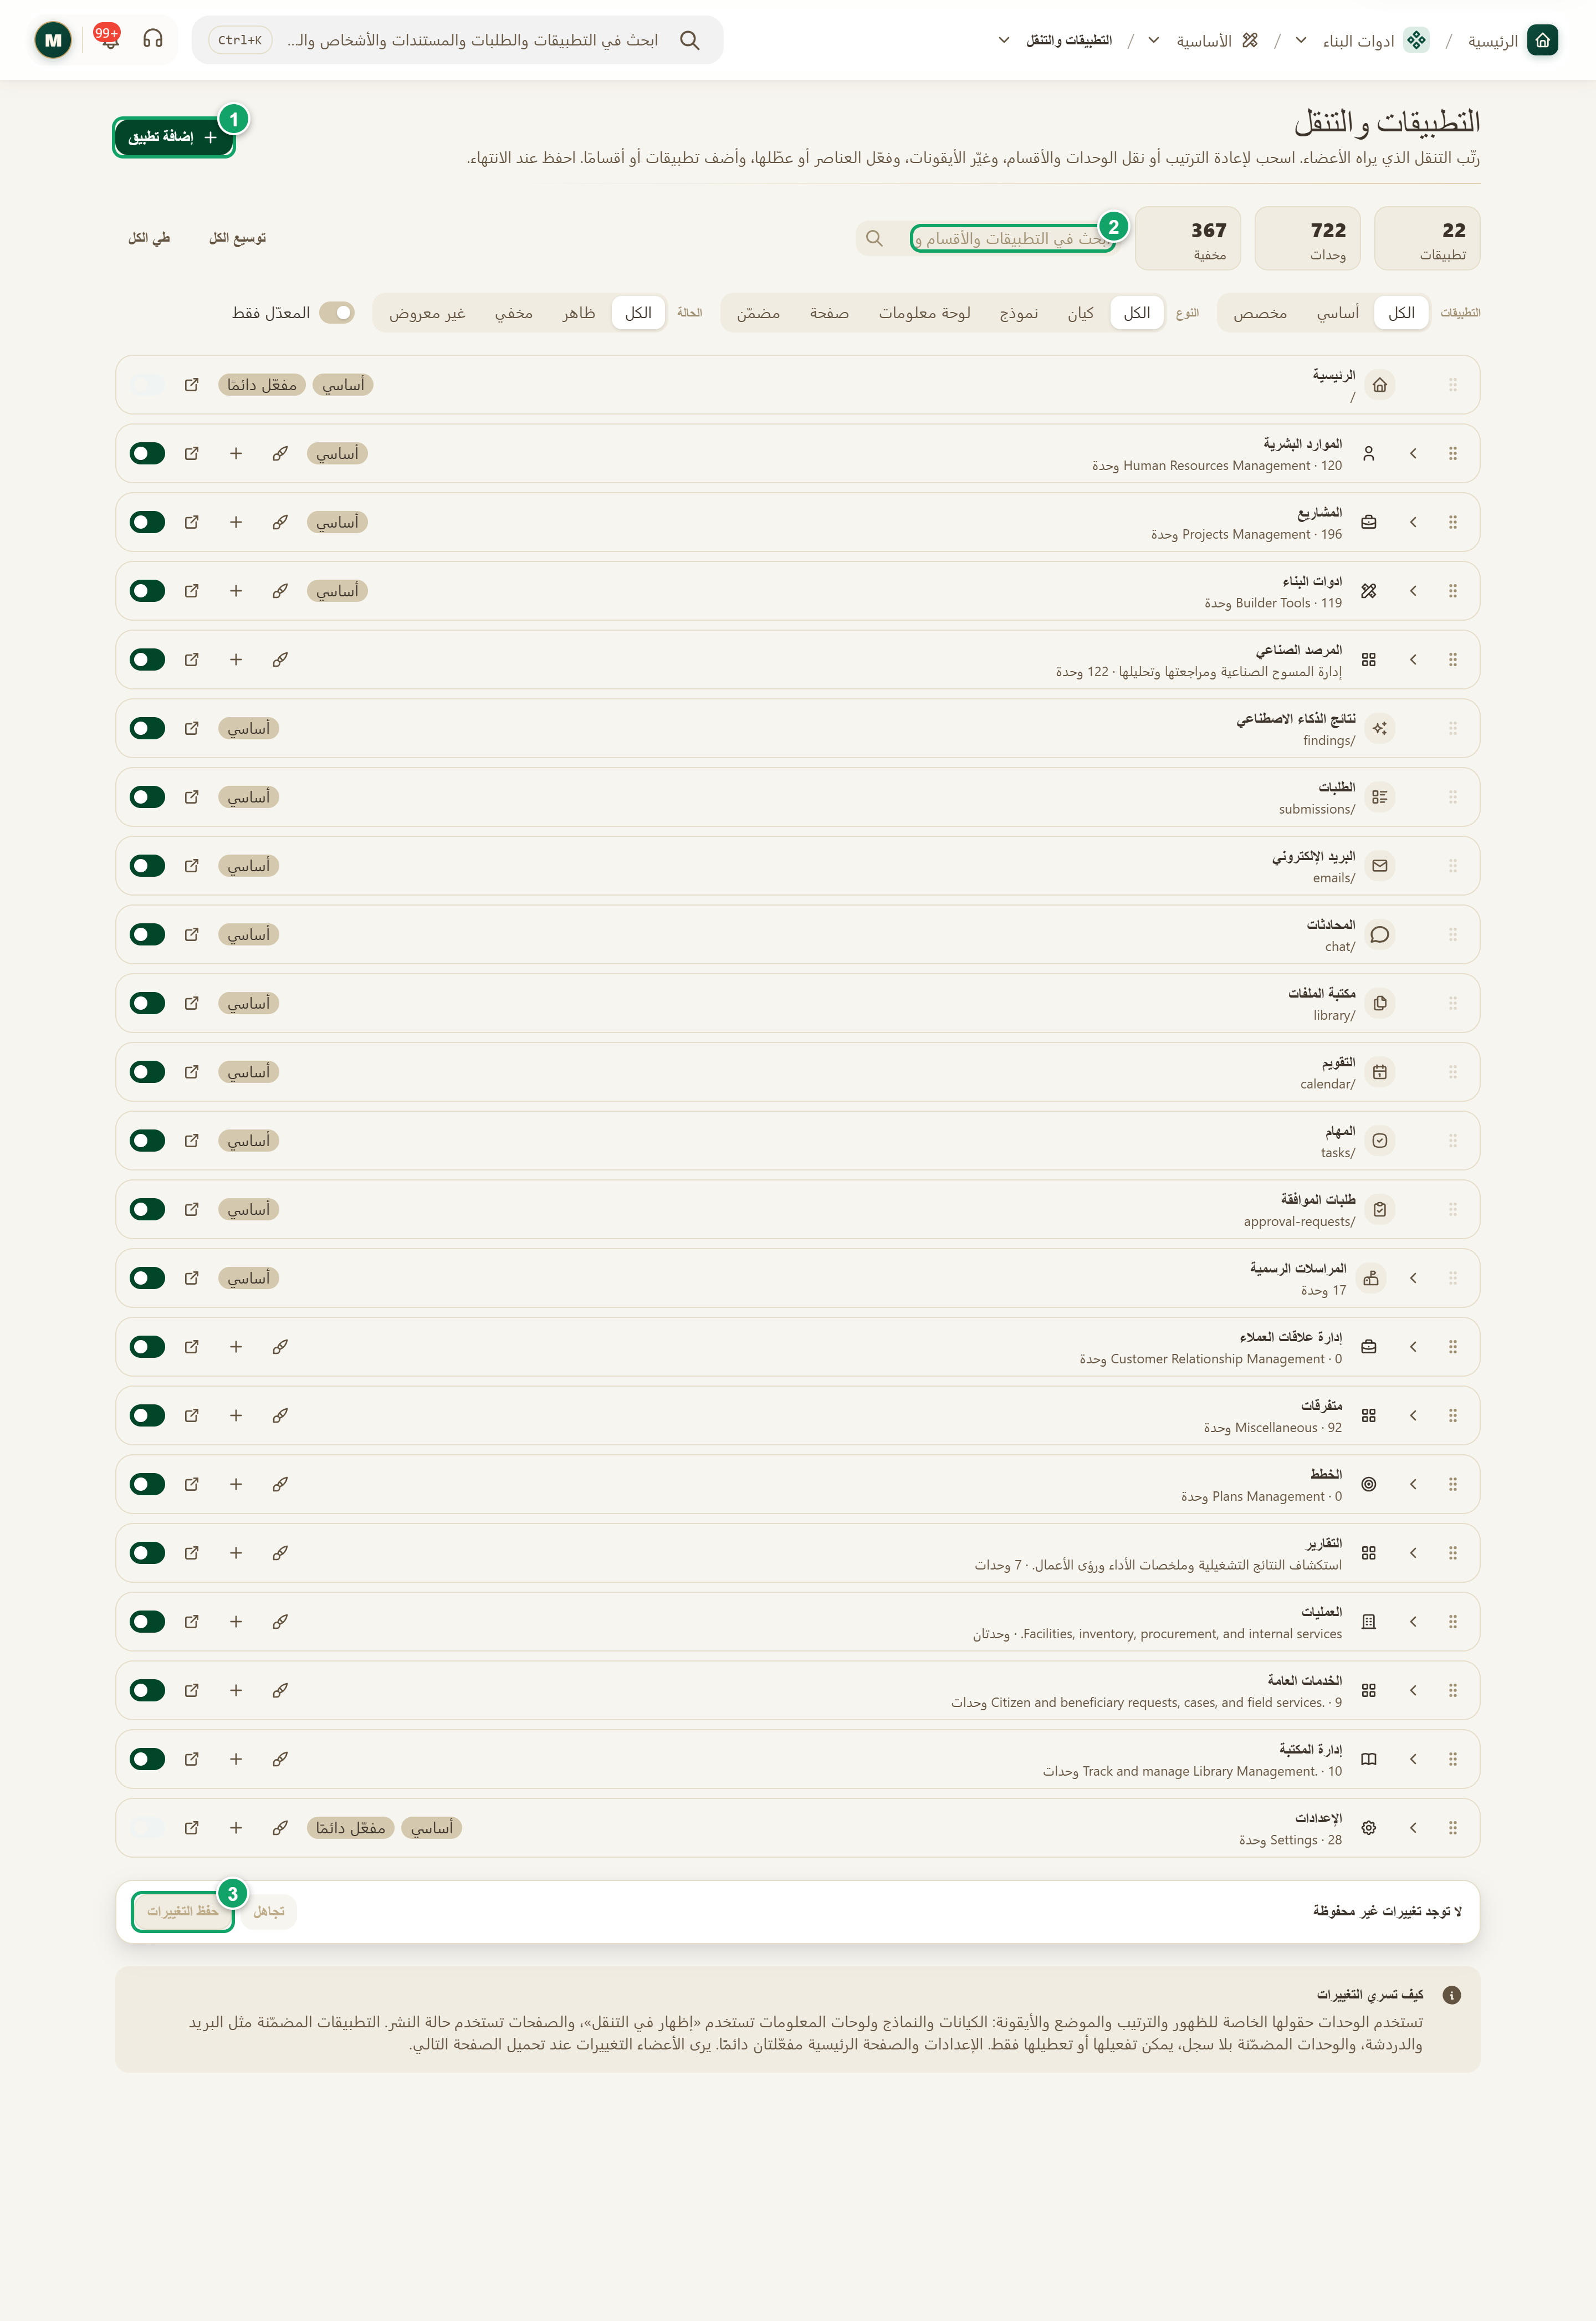
\includegraphics[width=0.95\linewidth,height=0.72\textheight,keepaspectratio]{figures/screens/ch06-navigation-ar.png}
\caption{صفحة «التطبيقات والتنقل»}
\label{fig:builder-navigation-screen}
\shotnote{تعرض الصفحة كل التطبيقات والأقسام والوحدات التي يراها الأعضاء، مع حالة كل منها. والتطبيقات الظاهرة تطبيقات مؤسسة الاختبار. ① «إضافة تطبيق»: يُنشئ تطبيقاً جديداً. ② البحث: يجد التطبيق أو القسم أو الوحدة بسرعة. ③ «حفظ التغييرات»: يحفظ الترتيب والتفعيل، ولا يلزم للقسم الجديد.}
\end{figure}


\begin{table}[H]
\centering
\caption{ما الذي تجده هنا؟}
\label{tab:builder-navigation-data}
\begin{tabularx}{\linewidth}{R{3.6cm} Y}
\rcHeaderRow
\thh{الجزء} & \thh{المحتوى والإجراء}\\
إضافة تطبيق وإضافة قسم & تُنشئ تطبيقاً جديداً، أو قسماً داخل تطبيق. ويُحفظ القسم مباشرة دون الضغط على الحفظ.\\
السحب والأيقونات والتفعيل & أعد ترتيب التطبيقات والأقسام والوحدات بالسحب، وغيّر الأيقونة، وفعّل العنصر أو عطّله. تحتاج هذه التغييرات إلى «حفظ التغييرات».\\
التصفية & «التطبيقات»: الكل أو أساسي أو مخصص؛ و«النوع»: كيان أو نموذج أو لوحة معلومات أو صفحة أو مضمّن؛ و«الحالة»: ظاهر أو مخفي أو غير معروض؛ و«المعدّل فقط».\\
حفظ التغييرات وتجاهل & يحفظ الترتيب والتفعيل أو يتراجع عنهما. ويرى الأعضاء التغييرات عند تحميل الصفحة التالي.\\
العناصر المضمّنة & التطبيقات المضمّنة مثل البريد والدردشة يمكن تفعيلها أو تعطيلها فقط، أما الإعدادات والصفحة الرئيسية فمفعّلتان دائماً.\\
\end{tabularx}
\end{table}

\begin{figure}[H]
\centering
\begin{tikzpicture}[node distance=0.5cm]
\node[entity] (app) {\RL{التطبيق}};
\node[entity,below=0.7cm of app] (section) {\RL{القسم}};
\node[entityOpt,below right=0.7cm and 0.3cm of section] (type) {\RL{نوع سجلات أو نموذج}};
\node[entityOpt,below left=0.7cm and 0.3cm of section] (dash) {\RL{لوحة معلومات أو صفحة}};
\draw[dependsOn] (app) -- (section);
\draw[dependsOnOpt] (section.south) -- ++(0,-0.3) -| (type.north);
\draw[dependsOnOpt] (section.south) -- ++(0,-0.3) -| (dash.north);
\end{tikzpicture}
\rclegend
\caption{كيف يُبنى التنقل}
\label{fig:builder-navigation-tree}
\shotnote{يوضّح الشكل أن التطبيق يضم أقساماً، وأن القسم يضم الوحدات التي يفتحها الأعضاء، مثل أنواع السجلات والنماذج ولوحات المعلومات. لذلك أنشئ التطبيق والقسم أولاً ثم اسحب الوحدة إليه؛ فالتطبيق المضمّن لا يستقبل وحدات جديدة.}
\end{figure}

\subsection{خطوات العمل والتحقق}
\begin{enumerate}
\item افتح «التطبيقات والتنقل»، واضغط «إضافة تطبيق» إن لم يكن للعمل تطبيق مناسب.
\item أضف قسماً من زر الإضافة في صف التطبيق، واختر له اسماً وأيقونة.
\item ابحث عن نوع السجلات أو النموذج، واسحبه إلى القسم، وتأكد من أنه «ظاهر».
\item اضغط «حفظ التغييرات».
\end{enumerate}

\textbf{تحقق ومعالجة المشكلة:} يجب أن تظهر رسالة «تم حفظ التنقل»، وأن يظهر التطبيق للأعضاء بعد تحميل الصفحة من جديد. فإذا لم يظهر لعضو، فتأكد من أن لديه صلاحية رؤية السجلات، لأن القسم الذي لا يحتوي عنصراً مسموحاً له لا يظهر. وإذا رفضت الصفحة نقل وحدة، فانقلها إلى قسم غير مضمّن.

\clearpage
\section{التنقل حسب العمل}
\label{sec:builder-feature-work-navigation}

تحدد هذه الصفحة ما يراه كل عضو أولاً عندما يبدأ يومه: صفحة «مكتبي» بحسب دوره، وقائمة «المستحق عليّ» التي تجمع ما ينتظره من عمل، وسياقاً مشتركاً مثل السنة أو الدورة تتبعه القوائم واللوحات، وطرق عرض محفوظة تظهر في القوائم بعدّاداتها. وكل ميزة فيها متوقفة حتى تفعّلها.

\textbf{المسار ومن يستخدمه:} «ادوات البناء» ← «الأساسية» ← «التنقل حسب العمل». تظهر لمالك المؤسسة ومسؤولها فقط.

\begin{rcnote}[مثال: شركة الأفق]
يفعّل مسؤول النظام «قائمة المستحق عليّ»، ويضيف إليها طلبات الزيارة التي تنتظر قرار سارة الخطيب، فتجدها سارة في مكان واحد كل صباح بدلاً من فتح كل قائمة على حدة. ويفعّل الميزة من ① ثم يضيف المصدر من ②.
\end{rcnote}

\begin{figure}[H]
\centering
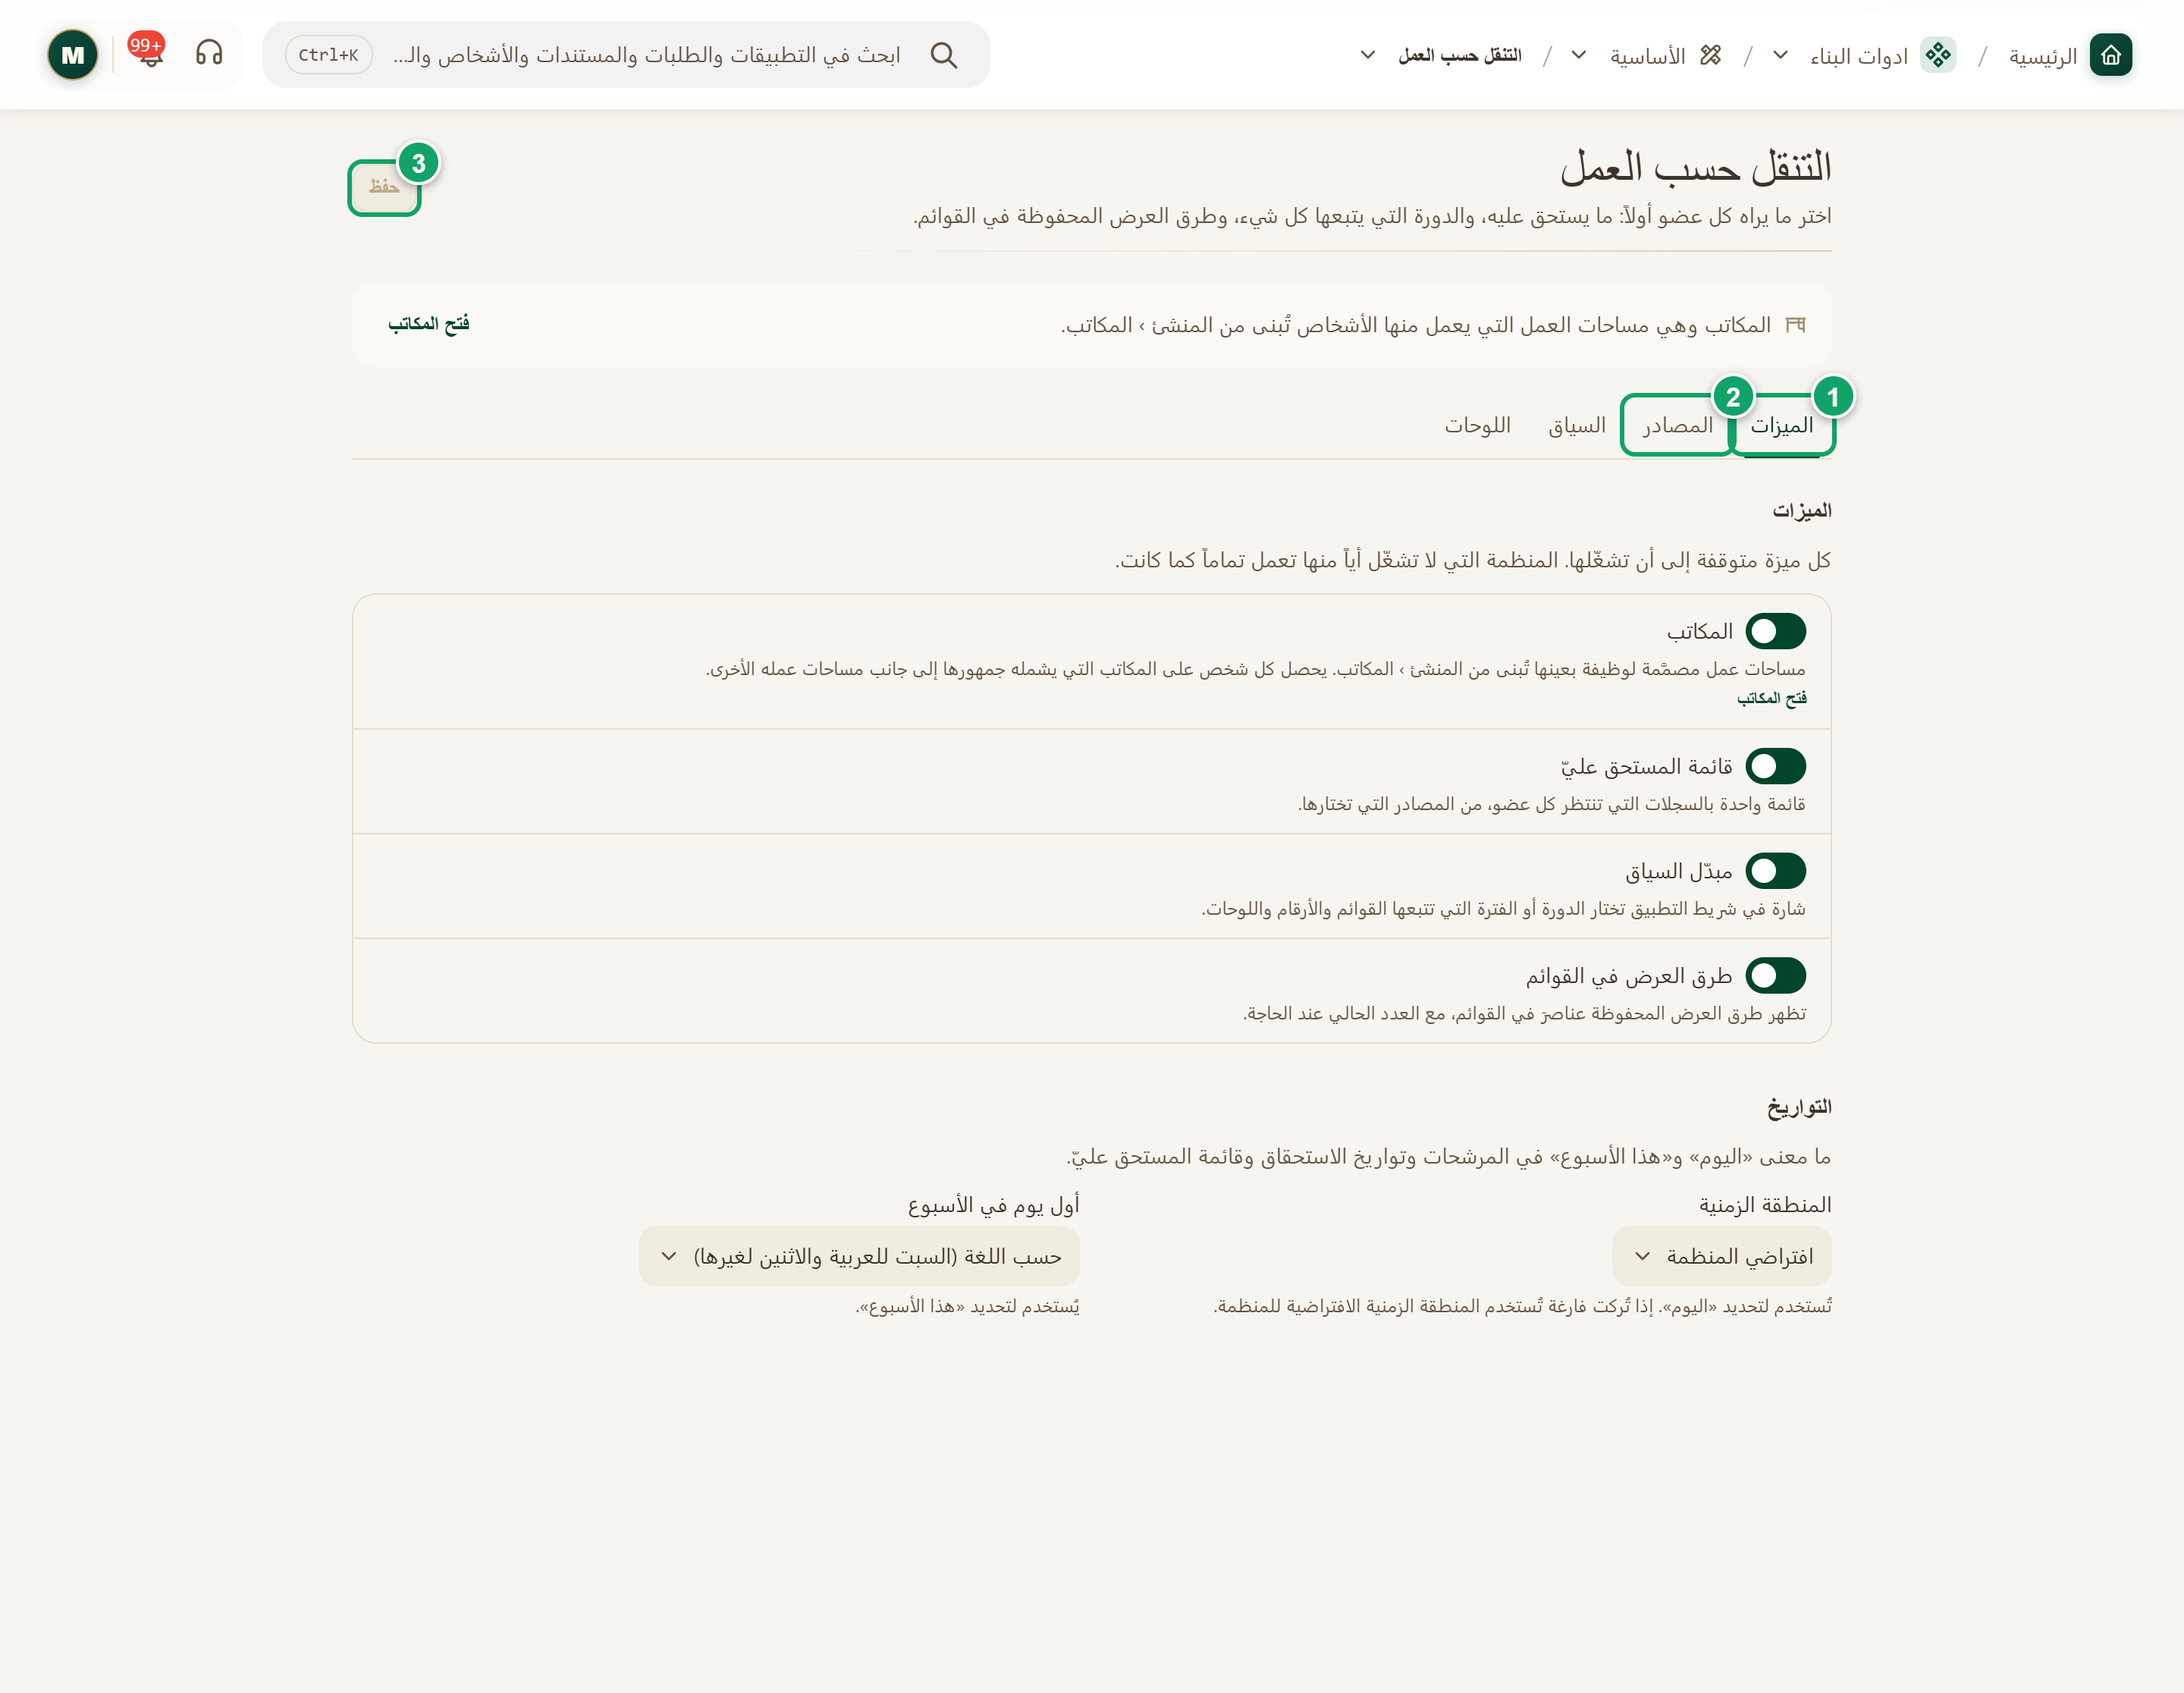
\includegraphics[width=0.95\linewidth,height=0.72\textheight,keepaspectratio]{figures/screens/ch06-work-navigation-ar.png}
\caption{صفحة «التنقل حسب العمل»}
\label{fig:builder-work-navigation-screen}
\shotnote{تعرض الصفحة ميزات صفحة البداية والمستحقات، وكلها متوقفة حتى تفعّلها. ① «الميزات»: تشغيل «صفحة مكتبي» و«قائمة المستحق عليّ» وغيرهما. ② «المصادر»: ما يغذّي قائمة المستحق. ③ «حفظ»: يحفظ الإعدادات، ويكون معطلاً حتى تغيّر شيئاً.}
\end{figure}


\begin{table}[H]
\centering
\caption{تبويبات الصفحة}
\label{tab:builder-work-navigation-data}
\begin{tabularx}{\linewidth}{R{3.6cm} Y}
\rcHeaderRow
\thh{التبويب} & \thh{ماذا تحدد؟}\\
الميزات & تشغيل «صفحة مكتبي» و«قائمة المستحق عليّ» و«مبدّل السياق» و«طرق العرض في القوائم»، مع التقويم والمنطقة الزمنية وبداية الأسبوع.\\
المصادر & ما يغذّي قائمة «المستحق عليّ»: الانتقالات التي يستطيع العضو تنفيذها، والسجلات المسندة إليه، والقوائم المدمجة مثل الموافقات.\\
الصفحات & صفحات «مكتبي» لكل دور ولبقية الأعضاء. وهي صفحات بداية لا تظهر في القوائم، وتختلف عن صفحة «الصفحات».\\
السياق & نوع سجلات، مثل السنة أو الدورة، تتبعه تطبيقات وأقسام تختارها، فيختاره العضو من شريحة في شريط التطبيق.\\
اللوحات & نطاق البيانات الافتراضي للوحات الجديدة، وقائمة باللوحات التي تعرض بيانات المؤسسة كاملة لتحويلها إلى صلاحيات المشاهد.\\
\end{tabularx}
\end{table}

\begin{figure}[H]
\centering
\begin{tikzpicture}[node distance=0.5cm]
\node[entity] (member) {\RL{العضو}};
\node[entityOpt,below right=0.7cm and 0.3cm of member] (desk) {\RL{صفحة مكتبي}};
\node[entityOpt,below left=0.7cm and 0.3cm of member] (due) {\RL{المستحق عليّ}};
\draw[dependsOnOpt] (member.south) -- ++(0,-0.3) -| (desk.north);
\draw[dependsOnOpt] (member.south) -- ++(0,-0.3) -| (due.north);
\end{tikzpicture}
\rclegend
\caption{ما يراه العضو أولاً}
\label{fig:builder-work-navigation-model}
\shotnote{يوضّح الشكل أن هذه الصفحة لا تُنشئ بيانات جديدة، بل تقرّب العمل الموجود من العضو: صفحة بداية تناسب دوره، وقائمة تجمع ما يستحق عليه من أنواع سجلات مختلفة. وكلاهما اختياري، لذلك فعّل ميزة واحدة وجرّبها قبل تفعيل غيرها.}
\end{figure}

\subsection{خطوات العمل والتحقق}
\begin{enumerate}
\item افتح «التنقل حسب العمل»، وفعّل في «الميزات» ما تحتاجه المؤسسة.
\item أضف في «المصادر» ما يجب أن يظهر في قائمة «المستحق عليّ».
\item أنشئ صفحة «مكتبي» للدور المناسب من «الصفحات» عند الحاجة، ثم اضغط «حفظ».
\end{enumerate}

\textbf{تحقق ومعالجة المشكلة:} يجب أن تظهر رسالة «تم حفظ التنقل حسب العمل»، وأن يرى العضو صفحته وقائمته بعد تحميل الصفحة. فإذا ظهرت «إعدادات تحتاج إلى مراجعة»، فهناك إعداد يشير إلى نوع سجلات أو حقل تغيّر أو حُذف؛ فافتحه وصحّحه قبل الحفظ.

\clearpage
\section{النماذج}
\label{sec:builder-feature-forms}

النموذج صفحة أسئلة يعبّئها موظف أو مقدّم طلب، مثل طلب إجازة أو استمارة زيارة. وتنشئ النماذج وتنشر إصداراتها من صفحة «النماذج»، ويمكن أن يكتب النموذج إجاباته في نوع سجلات، وأن يكون له مسار حالات واعتماد. ويعمل الناس دائماً على الإصدار المنشور، بينما تعدّل أنت مسودة جديدة دون أن تؤثر فيهم.

\textbf{المسار ومن يستخدمه:} «ادوات البناء» ← «الأساسية» ← «النماذج». يستخدمها من يملك صلاحية النماذج لتصميم طريقة جمع الطلبات.

\begin{rcnote}[مثال: شركة الأفق]
يبني مسؤول النظام نموذج «طلب زيارة فرع» يسأل عن الفرع والموعد والغرض، ويجعله يكتب الإجابات في «طلبات الزيارة» عند اعتماد سارة الخطيب للطلب، فيعبّئه عمر حداد دون أن يفتح نوع السجلات نفسه. ويبدأ النموذج من ①.
\end{rcnote}

\begin{figure}[H]
\centering
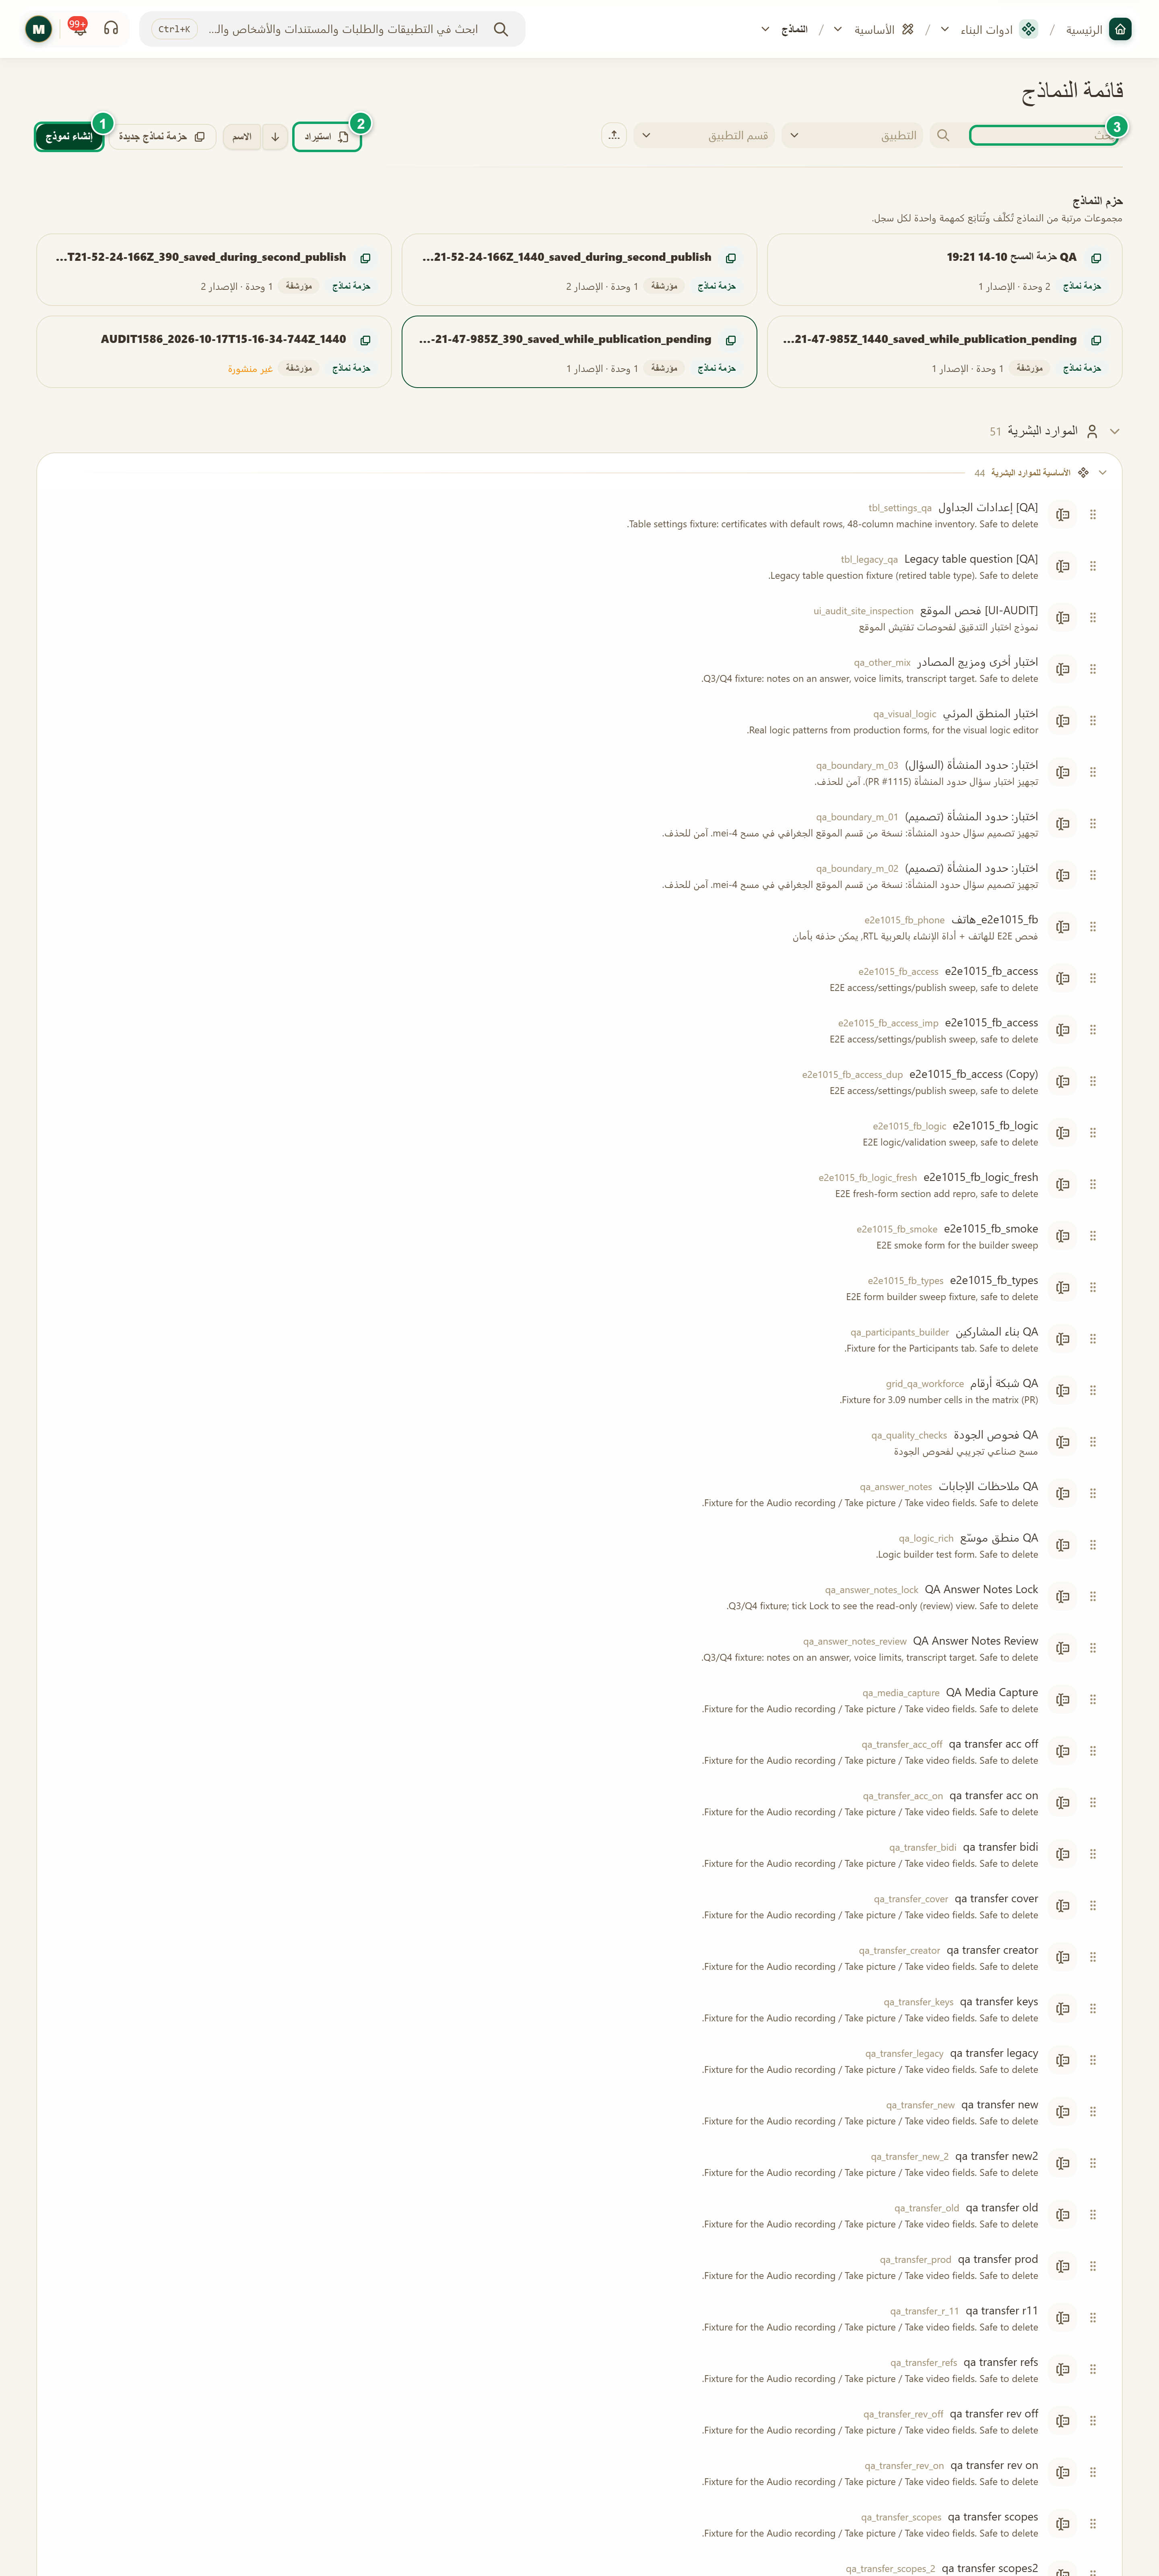
\includegraphics[width=0.95\linewidth,height=0.72\textheight,keepaspectratio]{figures/screens/ch06-forms-ar.png}
\caption{صفحة «النماذج»}
\label{fig:builder-forms-screen}
\shotnote{تعرض الصفحة النماذج مجمّعة حسب التطبيق والقسم مع عدد الطلبات لكل نموذج. والنماذج الظاهرة نماذج اختبار في test2. ① «إنشاء نموذج»: يبدأ نموذجاً جديداً. ② «استيراد»: يُنشئ نموذجاً من ملف مُصدَّر. ③ البحث: يجد النموذج بالاسم.}
\end{figure}


\begin{table}[H]
\centering
\caption{قائمة النماذج}
\label{tab:builder-forms-list}
\begin{tabularx}{\linewidth}{R{3.6cm} Y}
\rcHeaderRow
\thh{الجزء} & \thh{المحتوى والإجراء}\\
إنشاء نموذج & يطلب «اسم النموذج» و«كود النموذج» و«الاختصار المرجعي» والتطبيق والقسم، ثم يفتح المنشئ.\\
القائمة & النماذج مجمّعة حسب التطبيق والقسم، مع البحث والترتيب وعدد الطلبات، وإجراءات «نسخ» و«تصدير النموذج» و«حذف النموذج».\\
استيراد & يُنشئ نموذجاً من ملف مُصدَّر سابقاً.\\
حزم النماذج & مجموعات مرتبة من النماذج تُكلَّف وتُتابَع كمهمة واحدة لكل سجل.\\
\end{tabularx}
\end{table}

\begin{table}[H]
\centering
\caption{أدوات منشئ النموذج}
\label{tab:builder-forms-editor}
\begin{tabularx}{\linewidth}{R{3.6cm} Y}
\rcHeaderRow
\thh{الأداة} & \thh{ماذا تفعل؟}\\
الأسئلة & تضيف الأسئلة من مجموعات: نص، واختيار، وأرقام وتقييم، وتاريخ ووقت، وموقع، والملفات والوسائط، وأخرى؛ مع أقسام وصفحات ونص كتابي.\\
القواعد & كل ما يُظهر سؤالاً أو يخفيه أو يقفله أو يلزم به أو يحسبه أو يتحقق منه، في قائمة واحدة.\\
الوصول & من يستطيع الوصول إلى كل رد، وماذا يستطيع أن يفعل به: من يبدأ النموذج، أو أشخاص ثابتون، أو أشخاص تحددهم الإجابات.\\
المسار & «مسار الطلب»: الحالات والمراحل التي يراها مقدّم الطلب، والانتقالات بينها، وخطوات الموافقة.\\
السجلات & السجلات التي يقرأ منها النموذج ويكتب إليها، ومتى يكتب: «عند الاعتماد» أو «عند الإرسال».\\
إسناد & خطط تكلّف أشخاصاً بتعبئة النموذج لسجلات معينة، وتظهر بعد حفظ النموذج.\\
الإصدارات والإعدادات & «سجل الإصدارات» لكل إصدار، والإعدادات مثل الترقيم ومستند PDF والروابط المملوءة مسبقاً.\\
اختبار النموذج ونشر & يفتح مساحة اختبار معزولة تجرّب فيها النموذج بصفة عضو، ثم «نشر» يجعل المسودة الإصدار المنشور.\\
\end{tabularx}
\end{table}

\begin{figure}[H]
\centering
\begin{tikzpicture}[node distance=0.5cm]
\node[stepBox] (a) {\RL{إنشاء نموذج}};
\node[stepBox,below=of a] (b) {\RL{الأسئلة والقواعد}};
\node[stepBox,below=of b] (c) {\RL{الوصول والمسار والسجلات}};
\node[stepBox,below=of c] (d) {\RL{اختبار النموذج}};
\node[stepBox,below=of d] (e) {\RL{نشر}};
\draw[flowsTo] (a) -- (b);
\draw[flowsTo] (b) -- (c);
\draw[flowsTo] (c) -- (d);
\draw[flowsTo] (d) -- (e);
\end{tikzpicture}
\rclegend
\caption{من الفكرة إلى نموذج منشور}
\label{fig:builder-forms-flow}
\shotnote{يرتّب المخطط بناء النموذج من محتواه إلى سلوكه: الأسئلة أولاً، ثم من يصل إلى الرد وأين تذهب الإجابات. ويأتي الاختبار قبل النشر لأن مساحة الاختبار معزولة، فتكشف الخطأ دون أن يصل إلى أحد؛ أما النشر فيجعل الإصدار متاحاً لكل من يعبّئ النموذج.}
\end{figure}

\subsection{خطوات العمل والتحقق}
\begin{enumerate}
\item افتح «النماذج» واضغط «إنشاء نموذج»، ثم اكتب الاسم والكود والاختصار واختر التطبيق والقسم.
\item أضف الأسئلة، واختر لكل منها نوعاً يناسب الإجابة، ثم أضف القواعد عند الحاجة.
\item افتح «الوصول» لتحدد من يرى الردود، و«السجلات» إن أردت أن تُكتب الإجابات في نوع سجلات.
\item اضغط «اختبار النموذج» وعبّئه كاملاً، ثم اضغط «نشر».
\end{enumerate}

\textbf{تحقق ومعالجة المشكلة:} يجب أن تظهر رسالة «تم نشر النموذج بنجاح»، وأن يظهر الإصدار «منشور» في «سجل الإصدارات». فإذا تحوّل زر النشر إلى «إرسال للاعتماد»، فمؤسستك تشترط اعتماد النشر، وسيُنشر النموذج بعد موافقة المعتمد. وإذا لم تُكتب الإجابات في السجل، فافتح «السجلات» وتأكد من موافقة مسؤول نوع السجلات على كتابة النموذج فيه.

\clearpage
\section{الخدمات}
\label{sec:builder-feature-services}

الخدمة هي ما يظهر للجمهور على بوابة المؤسسة، مثل «طلب شهادة» أو «حجز موعد». وتضم كل خدمة نموذجاً أو أكثر، وتحدد طريقة تقديمها ومن يحق له التقديم. لذلك لا يصل النموذج إلى المتعاملين إلا عبر خدمة، أما النموذج الذي لا ينتمي إلى خدمة فيبقى «نموذجاً داخلياً» للموظفين فقط.

\textbf{المسار ومن يستخدمه:} «ادوات البناء» ← «الأساسية» ← «الخدمات». يستخدمها من يدير الخدمات العامة للمؤسسة.

\begin{rcnote}[مثال: شركة الأفق]
تقبل الأفق طلبات صيانة من عملائها في حلب، فينشئ مسؤول النظام خدمة «طلب صيانة» تبدأ بنموذج منشور، ويجعلها متاحة لأصحاب الحسابات المسجّلة فقط. أما نموذج «طلب زيارة فرع» فيبقى نموذجاً داخلياً. ويبدأ الخدمة من ①، ويبقى نموذج الزيارة في ④.
\end{rcnote}

\begin{figure}[H]
\centering
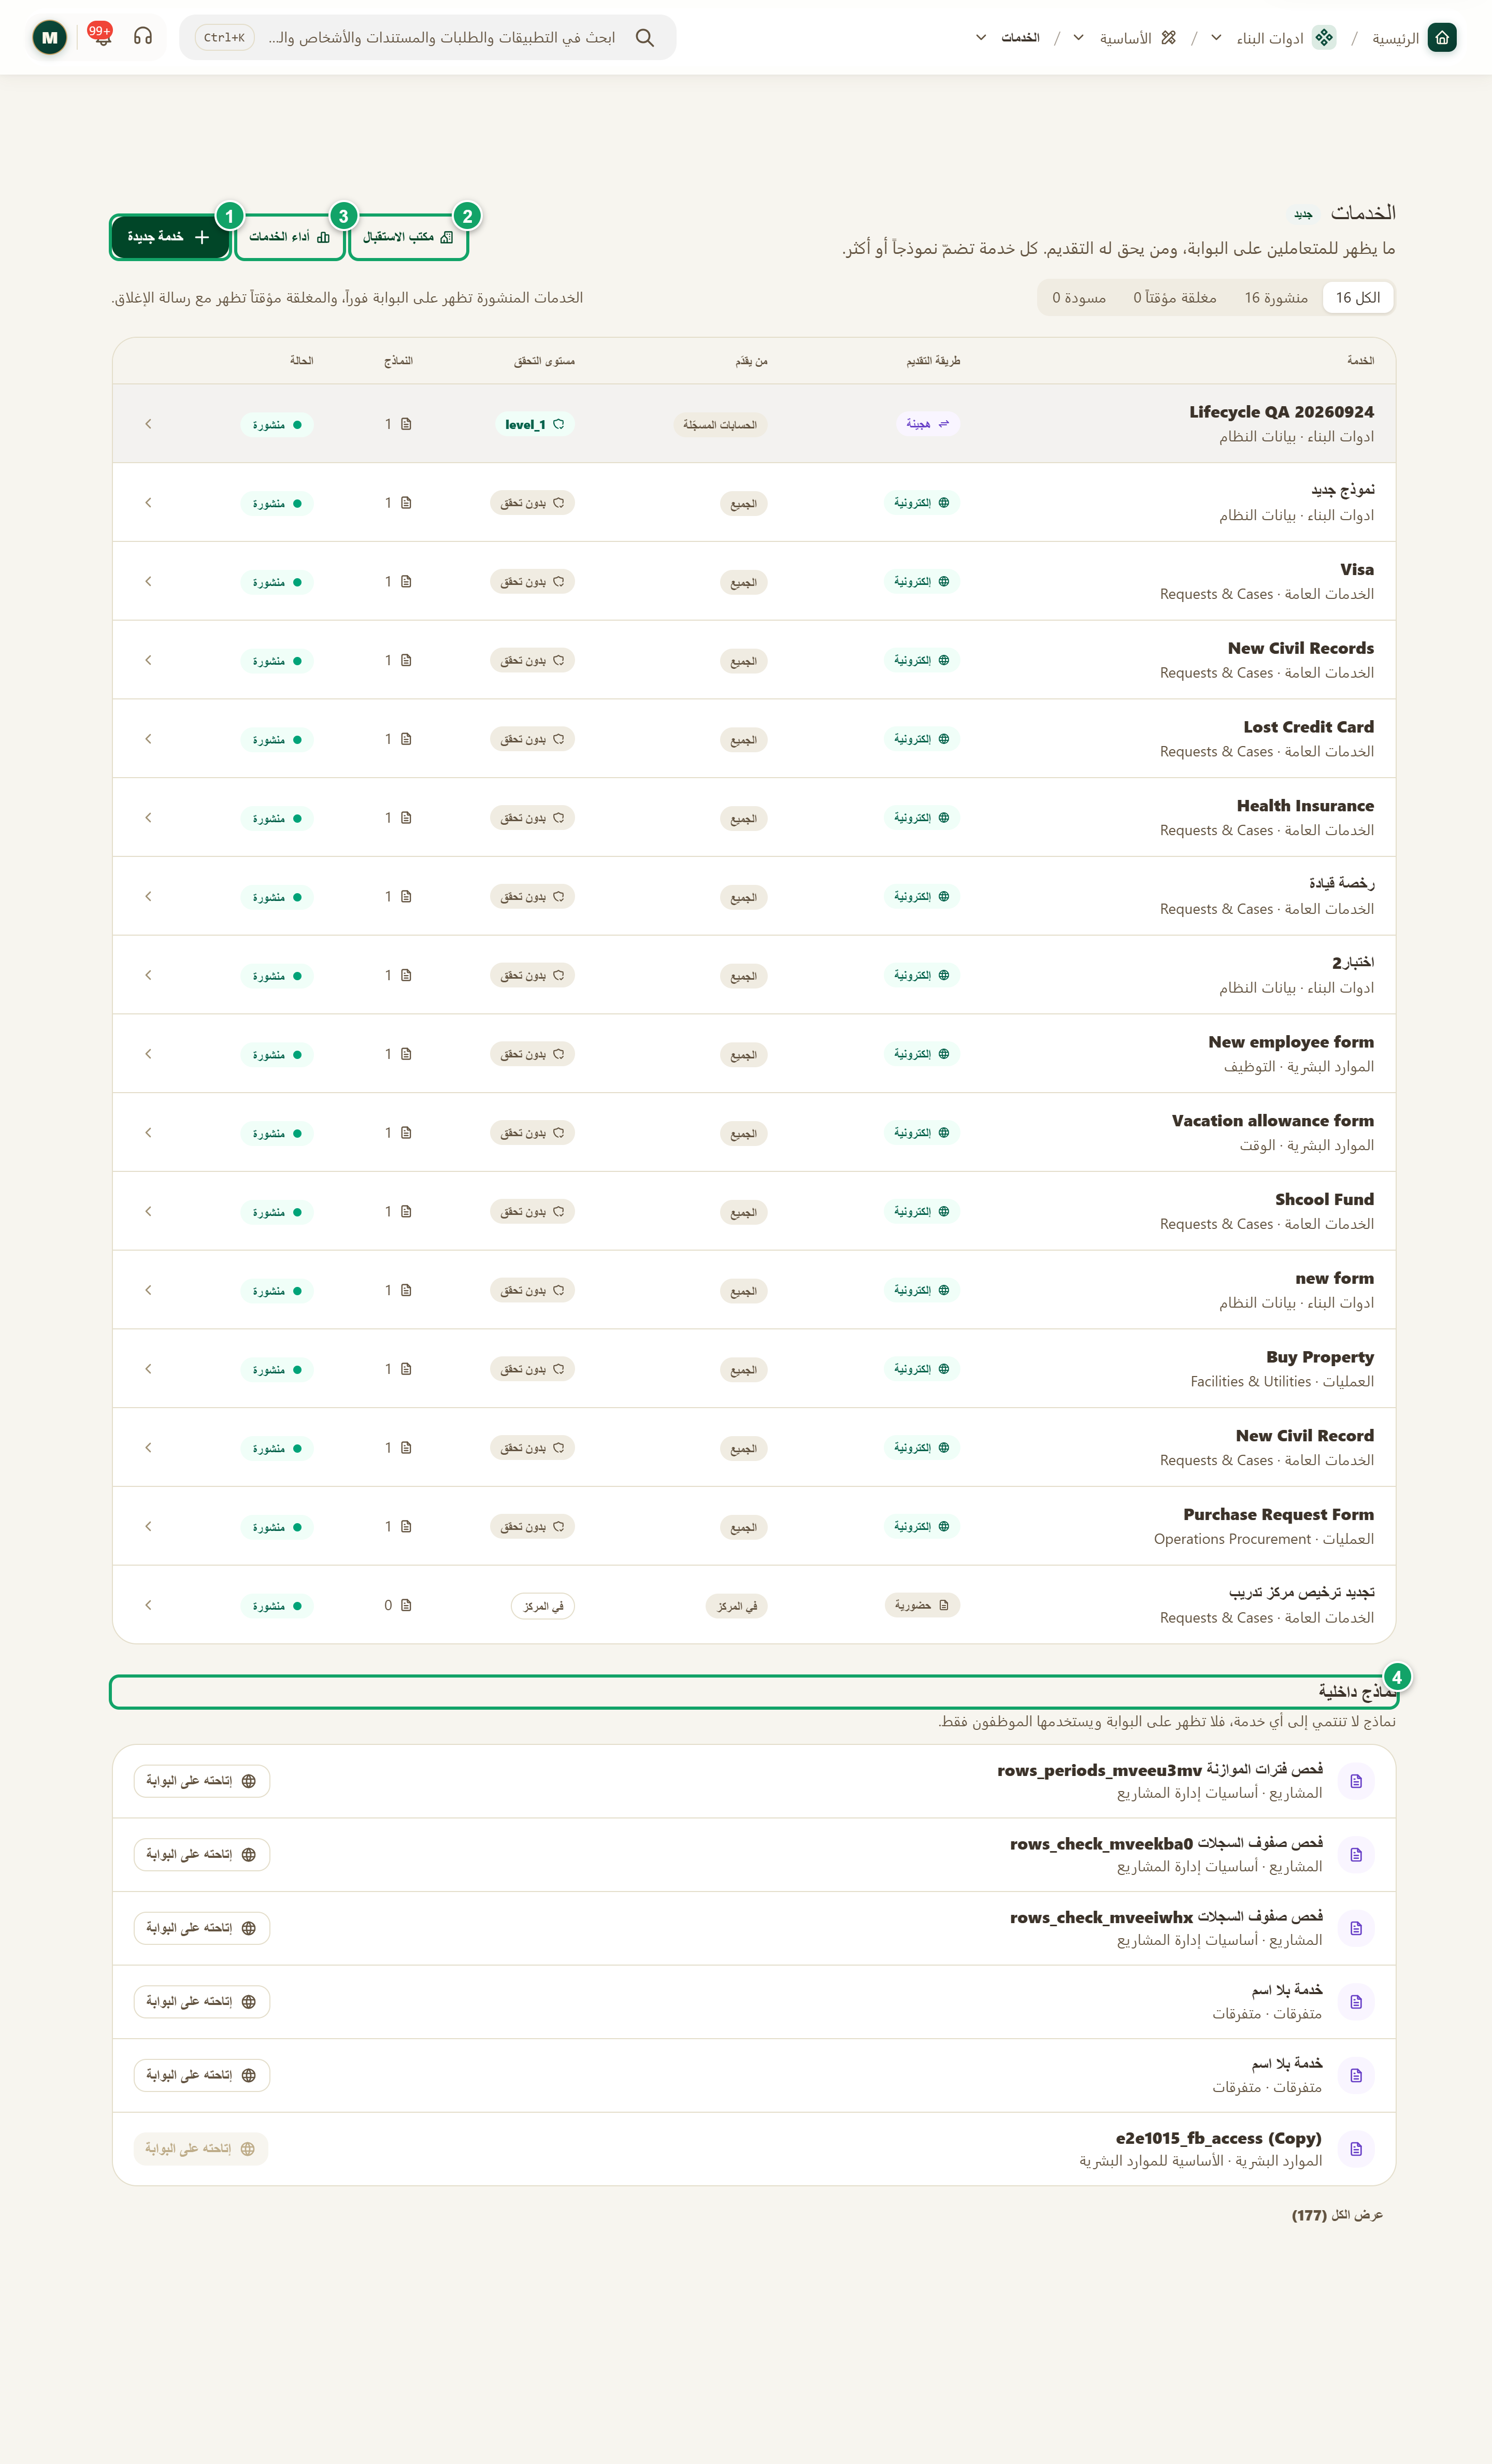
\includegraphics[width=0.95\linewidth,height=0.72\textheight,keepaspectratio]{figures/screens/ch06-services-ar.png}
\caption{صفحة «الخدمات»}
\label{fig:builder-services-screen}
\shotnote{تعرض الصفحة الخدمات التي تظهر على البوابة وحالتها، ثم النماذج الداخلية التي لا تنتمي إلى خدمة. ① «خدمة جديدة»: تبدأ خدمة حول نموذج منشور. ② «مكتب الاستقبال»: يسجّل طلباً حضورياً. ③ «أداء الخدمات»: يعرض سير الطلبات. ④ «نماذج داخلية»: النماذج التي لا يراها الجمهور.}
\end{figure}


\begin{table}[H]
\centering
\caption{ما الذي تجده هنا؟}
\label{tab:builder-services-data}
\begin{tabularx}{\linewidth}{R{3.6cm} Y}
\rcHeaderRow
\thh{الجزء} & \thh{المحتوى والإجراء}\\
الخدمات & جدول الخدمات مع «طريقة التقديم» و«من يقدّم» و«مستوى التحقق» والنماذج والحالة، وتصفية حسب «منشورة» أو «مغلقة مؤقتاً» أو «مسودة».\\
خدمة جديدة & تطلب اسم الخدمة و«النموذج الذي يبدأ به المتعامل»، ونموذجاً اختيارياً يعبّئه الموظف.\\
نماذج داخلية & نماذج لا تنتمي إلى خدمة. وزر «إتاحته على البوابة» يحوّل النموذج المنشور إلى خدمة جديدة أو خطوة في خدمة قائمة.\\
صفحة الخدمة & تبويبات «نظرة عامة» و«الرسوم» و«التعريف» و«التقديم والأهلية» و«المسار والنماذج».\\
مكتب الاستقبال وأداء الخدمات & تسجيل طلب حضوري في مركز الخدمة، ومتابعة سير الطلبات وأين تتأخر.\\
\end{tabularx}
\end{table}

\begin{figure}[H]
\centering
\begin{tikzpicture}[node distance=0.5cm]
\node[entity] (service) {\RL{الخدمة}};
\node[entity,below right=0.7cm and 0.3cm of service] (entry) {\RL{نموذج البداية}};
\node[entityOpt,below left=0.7cm and 0.3cm of service] (more) {\RL{نماذج المسار والمتابعة}};
\draw[dependsOn] (service.south) -- ++(0,-0.3) -| (entry.north);
\draw[dependsOnOpt] (service.south) -- ++(0,-0.3) -| (more.north);
\end{tikzpicture}
\rclegend
\caption{ما تضمه الخدمة}
\label{fig:builder-services-model}
\shotnote{يوضّح الشكل أن الخدمة تحتاج إلى نموذج بداية منشور يعبّئه المتعامل، وأن بقية النماذج اختيارية، مثل خطوات لاحقة في المسار أو نموذج متابعة يُطلب عند حالة معينة. لذلك انشر النموذج في منشئ النماذج أولاً، ثم أنشئ الخدمة حوله.}
\end{figure}

\subsection{خطوات العمل والتحقق}
\begin{enumerate}
\item انشر النموذج الذي سيبدأ به المتعامل من صفحة «النماذج».
\item افتح «الخدمات» واضغط «خدمة جديدة»، واختر النموذج، ثم اضغط «إنشاء الخدمة».
\item أكمل «التعريف» الذي يقرؤه المتعامل، وحدد في «التقديم والأهلية» من يحق له التقديم.
\item انشر الخدمة، ثم اضغط «عرض على البوابة» لتراها كما يراها المتعامل.
\end{enumerate}

\textbf{تحقق ومعالجة المشكلة:} يجب أن تظهر الخدمة المنشورة على البوابة فوراً. فإذا لم تظهر، فتأكد من أنها ليست «مسودة»، لأن «المسودة لا تظهر على البوابة». وإذا أردت إيقاف الطلبات مؤقتاً، فاجعلها «مغلقة مؤقتاً» مع رسالة للمتعاملين بدلاً من حذفها.

\clearpage
\section{الإجراءات الداخلية}
\label{sec:builder-feature-internal-sops}

الإجراء الداخلي مسار عمل يبدأ بحدث تختاره، ثم ينفّذ خطوات متتالية: قد تكون خطوة بشرية مثل طلب موافقة أو توقيع أو إنشاء مهمة، أو خطوة آلية مثل إنشاء سجل أو إرسال إشعار. وتبني الإجراءات وتختبرها وتنشرها من هذه الصفحة دون أدوات خارجية.

\textbf{المسار ومن يستخدمه:} «ادوات البناء» ← «الأساسية» ← «الإجراءات الداخلية». يستخدمها من يصمم مسارات العمل في المؤسسة.

\begin{rcnote}[مثال: شركة الأفق]
يبني مسؤول النظام إجراء «اعتماد طلب الزيارة» يبدأ «عند إرسال نموذج» طلب الزيارة، فيرسل «طلب موافقة» إلى سارة الخطيب، ثم يُنشئ لعمر حداد مهمة تجهيز الزيارة إذا وافقت. ويبدأ الإجراء من ① ويتابعه من ②.
\end{rcnote}

\begin{figure}[H]
\centering
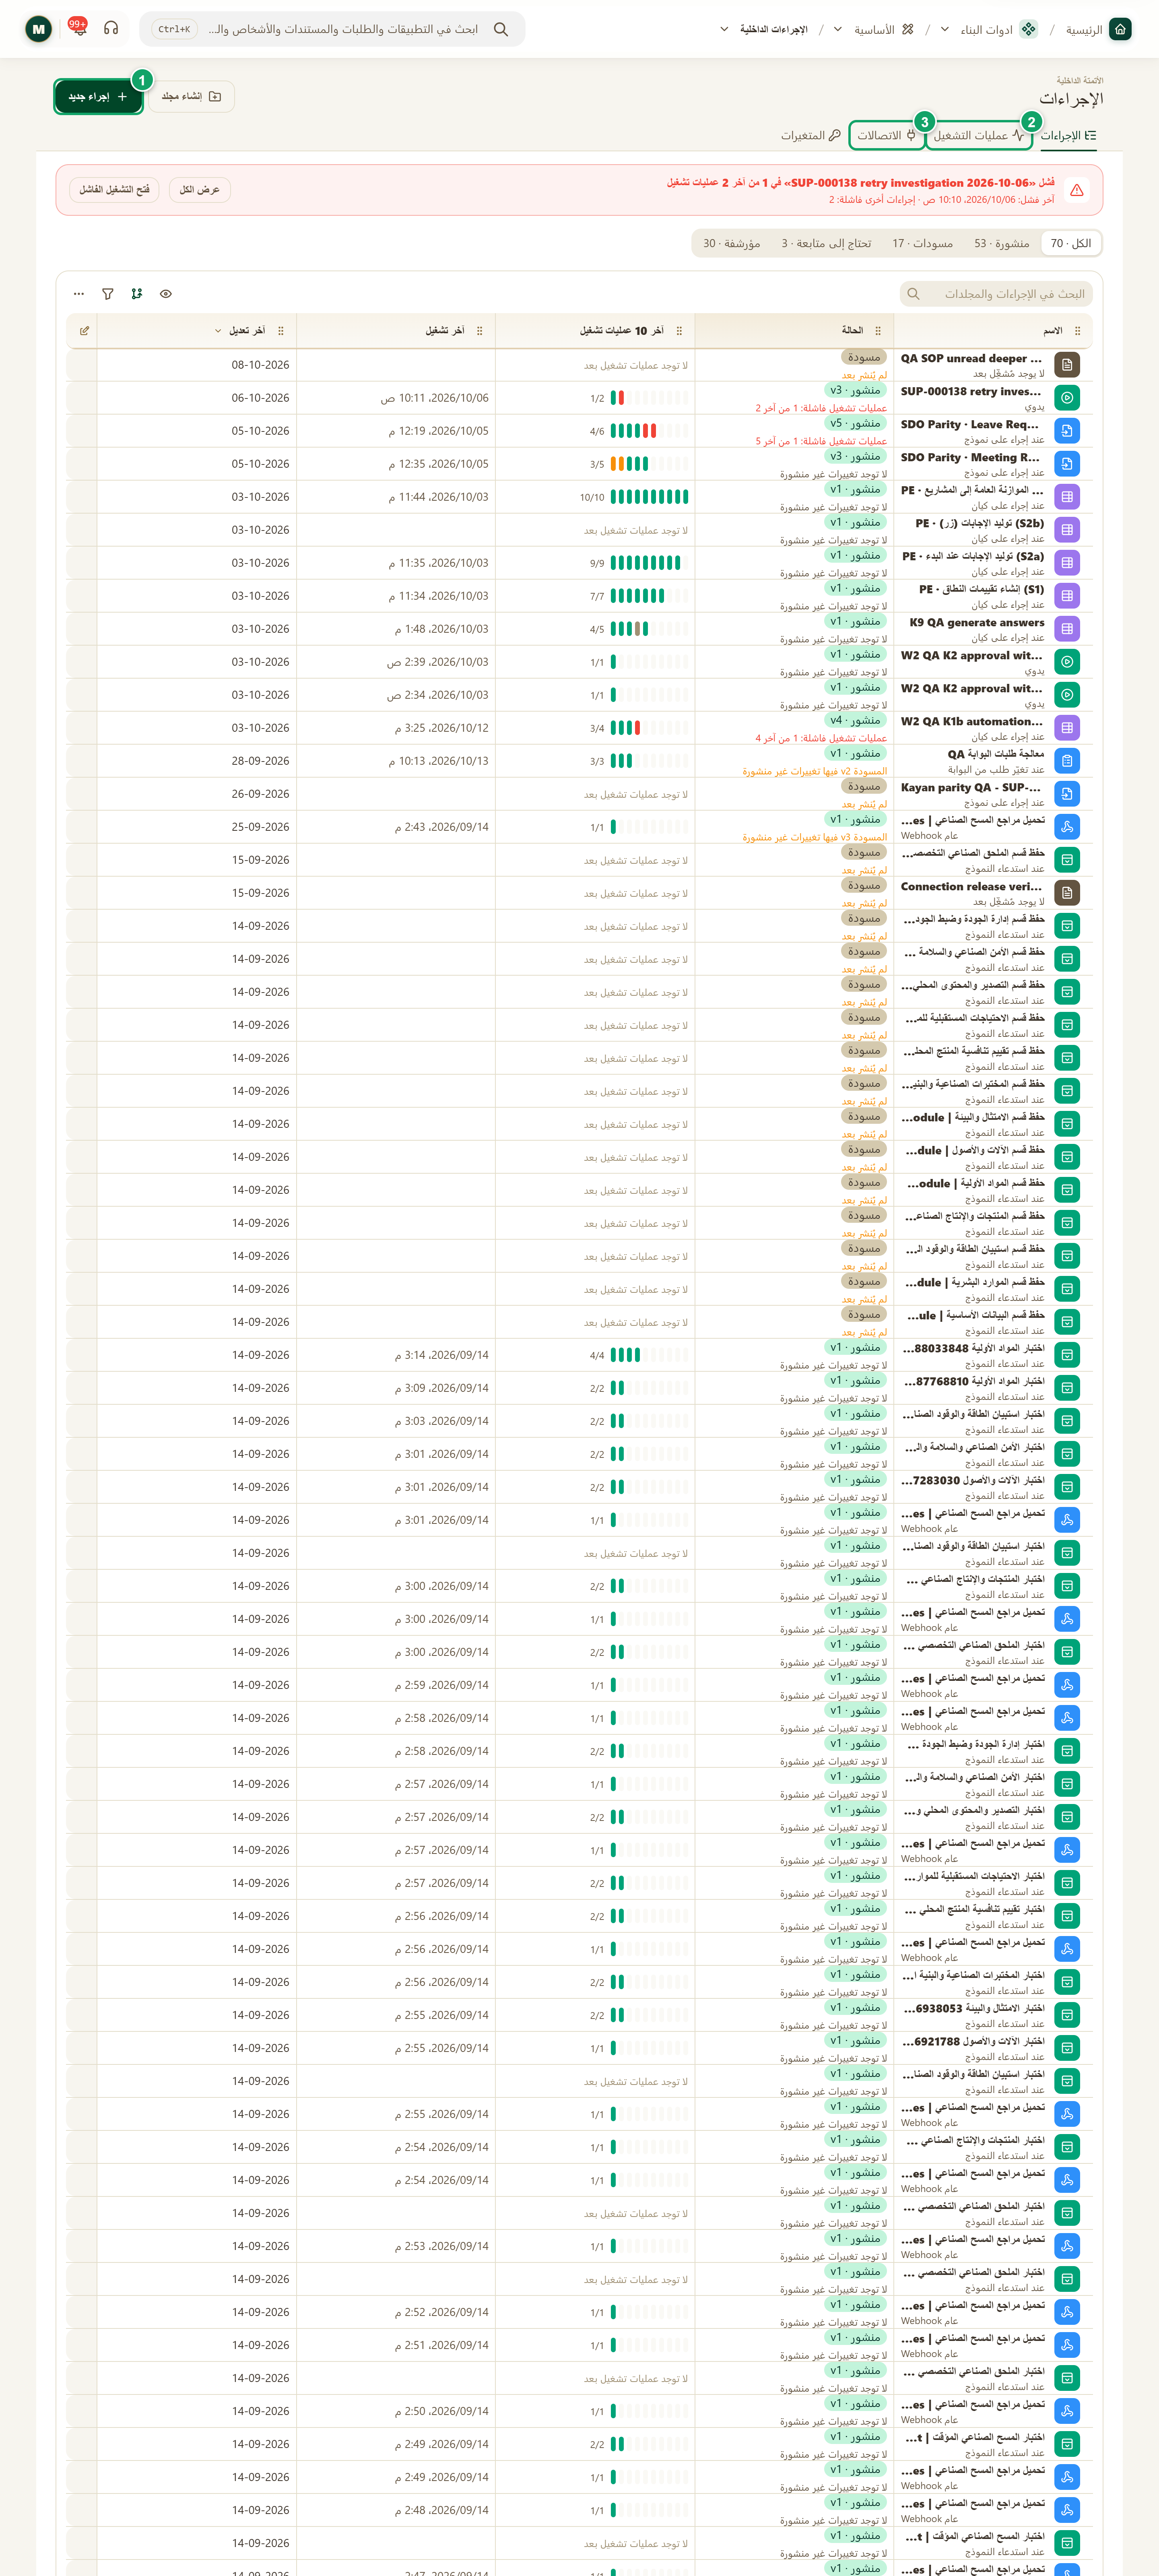
\includegraphics[width=0.95\linewidth,height=0.72\textheight,keepaspectratio]{figures/screens/ch06-internal-sops-ar.png}
\caption{صفحة «الإجراءات الداخلية»}
\label{fig:builder-internal-sops-screen}
\shotnote{تعرض الصفحة الإجراءات وحالاتها وتبويبات المتابعة. والقائمة فارغة في مؤسسة الاختبار. ① «إجراء جديد»: يبدأ إجراءً ويطلب ما الذي يبدأه. ② «عمليات التشغيل»: كل مرة عمل فيها إجراء ونتيجتها. ③ «الاتصالات»: حسابات الخدمات الخارجية التي تستخدمها الخطوات.}
\end{figure}


\begin{table}[H]
\centering
\caption{ما الذي تجده هنا؟}
\label{tab:builder-internal-sops-data}
\begin{tabularx}{\linewidth}{R{3.6cm} Y}
\rcHeaderRow
\thh{التبويب أو الأداة} & \thh{المحتوى والإجراء}\\
الإجراءات & قائمة الإجراءات مع حالتها ونتائج آخر عمليات التشغيل، وتصفية «منشورة» و«مسودات» و«تحتاج إلى متابعة» و«متوقفة مؤقتًا» و«مؤرشفة».\\
عمليات التشغيل & كل مرة بدأ فيها إجراء، مع حالتها: في قائمة الانتظار أو قيد التشغيل أو بانتظار استجابة أو مكتمل أو فاشل.\\
الاتصالات والمتغيرات & حسابات الخدمات الخارجية التي تستخدمها الخطوات، وقيم مشفّرة تستخدمها الإجراءات.\\
إجراء جديد & تكتب الاسم وتختار «ما الذي يبدأه؟»، مثل «عند إرسال نموذج» أو «إنشاء سجل جديد» أو «جدولة» أو «يدوي»، ثم «إنشاء وفتح».\\
المحرر & لوحة الخطوات مع أوضاع «بناء» و«اختبار» و«عمليات التشغيل». وتشمل الخطوات طلب موافقة ونموذج وتوقيع، وإنشاء مهمة، وتفرّعاً شرطياً، وانتظاراً، وإنشاء سجل أو تحديثه.\\
مراجعة ونشر & يعرض ما يجب إصلاحه والتغييرات منذ الإصدار المنشور، ثم ينشر إصداراً جديداً. وتكمل العمليات الجارية على إصدارها القديم.\\
\end{tabularx}
\end{table}

\begin{figure}[H]
\centering
\begin{tikzpicture}[node distance=0.5cm]
\node[stepBox] (a) {\RL{المشغّل: ما الذي يبدأه؟}};
\node[stepBox,below=of a] (b) {\RL{خطوات بشرية وآلية}};
\node[stepBox,below=of b] (c) {\RL{اختبار: محاكاة آمنة}};
\node[stepBox,below=of c] (d) {\RL{مراجعة ونشر}};
\node[stepBox,below=of d] (e) {\RL{متابعة عمليات التشغيل}};
\draw[flowsTo] (a) -- (b);
\draw[flowsTo] (b) -- (c);
\draw[flowsTo] (c) -- (d);
\draw[flowsTo] (d) -- (e);
\end{tikzpicture}
\rclegend
\caption{دورة حياة الإجراء الداخلي}
\label{fig:builder-internal-sops-flow}
\shotnote{يبيّن المخطط أن الإجراء لا يعمل إلا بعد نشره، وأن الاختبار يسبق النشر. فوضع «محاكاة (آمنة)» لا يُنشئ شيئاً فعلياً، بل يعيد بيانات مثال من الخطوات الخارجية، فتختبر المسار دون إزعاج أحد. وبعد النشر تتابع عمليات التشغيل لترى أين نجح الإجراء وأين توقف.}
\end{figure}

\subsection{خطوات العمل والتحقق}
\begin{enumerate}
\item افتح «الإجراءات الداخلية» واضغط «إجراء جديد»، ثم سمِّه واختر ما يبدأه واضغط «إنشاء وفتح».
\item أضف الخطوات على اللوحة، وأكمل إعداد كل خطوة حتى تظهر «كل الخطوات جاهزة».
\item انتقل إلى وضع «اختبار»، واختر «محاكاة (آمنة)»، ثم اضغط «تشغيل المحاكاة».
\item اضغط «مراجعة ونشر»، وراجع التغييرات، ثم انشر الإصدار.
\end{enumerate}

\textbf{تحقق ومعالجة المشكلة:} يجب أن تظهر حالة الإجراء «منشورة»، وأن تظهر عمليات التشغيل بعد وقوع الحدث. فإذا فشلت عملية، فافتحها من «عمليات التشغيل» لترى الخطوة التي فشلت، ثم أصلحها وانشر من جديد. وإذا أردت إيقاف الإجراء مؤقتاً، فأوقفه بدلاً من حذفه؛ فلن تبدأ عمليات جديدة حتى تستأنفه.

\clearpage
\section{إجراءات التشغيل القياسية}
\label{sec:builder-feature-sops}

تفتح هذه الصفحة استوديو أتمتة مضمّناً يبني مسارات تربط كيان بحسابات وخدمات أخرى، وتبدأ بحدث في كيان مثل إنشاء سجل أو إرسال نموذج. وتعمل كل أتمتة فيه من خلال اتصال بحساب كيان تختاره أولاً. أما مسارات الاعتماد والمهام داخل المؤسسة فالأنسب لها «الإجراءات الداخلية».

\textbf{المسار ومن يستخدمه:} «ادوات البناء» ← «الأساسية» ← «إجراءات التشغيل القياسية». يستخدمها من يملك صلاحية النماذج ويحتاج إلى ربط كيان بأنظمة أخرى.

\begin{rcnote}[مثال: شركة الأفق]
تريد الأفق أن تصل رسالة إلى جدول متابعة خارجي كلما أُنشئ طلب زيارة. لذلك يبني مسؤول النظام أتمتة تبدأ عند إنشاء سجل جديد في «طلبات الزيارة»، ثم تتحقق من الفرع قبل أن ترسل البيانات.
\end{rcnote}

\begin{table}[H]
\centering
\caption{أجزاء الأتمتة}
\label{tab:builder-sops-parts}
\begin{tabularx}{\linewidth}{R{3.6cm} Y}
\rcHeaderRow
\thh{الجزء} & \thh{المعنى}\\
الاتصال & حساب كيان الذي تعمل الأتمتة باسمه، ويُختار أولاً. اجعله بأقل صلاحيات تكفي العمل.\\
المشغّل & الحدث الذي يبدأ الأتمتة، مثل إنشاء سجل أو تحديثه أو إجراء على نموذج أو مهمة.\\
الشرط & يتحقق من البيانات قبل أي كتابة، حتى لا تعمل الأتمتة على سجلات لا تخصها.\\
الإجراءات & ما تفعله الأتمتة: إنشاء سجل أو تحديثه أو البحث عنه، وإنشاء مهام، وإرسال إشعار، وغيرها.\\
\end{tabularx}
\end{table}

\begin{figure}[H]
\centering
\begin{tikzpicture}[node distance=0.5cm]
\node[stepBox] (a) {\RL{اختيار الاتصال}};
\node[stepBox,below=of a] (b) {\RL{المشغّل}};
\node[stepBox,below=of b] (c) {\RL{شرط قبل الكتابة}};
\node[stepBox,below=of c] (d) {\RL{إجراء واحد في كل مرة}};
\draw[flowsTo] (a) -- (b);
\draw[flowsTo] (b) -- (c);
\draw[flowsTo] (c) -- (d);
\end{tikzpicture}
\rclegend
\caption{ترتيب بناء الأتمتة}
\label{fig:builder-sops-flow}
\shotnote{يضع المخطط الشرط قبل الإجراء، لأن الأتمتة التي تكتب دون تحقق قد تغيّر سجلات كثيرة في لحظة. وتُختبر الأجزاء واحداً واحداً: المشغّل وحده، ثم الشرط في الحالتين، ثم كل إجراء على حدة.}
\end{figure}

\subsection{خطوات العمل والتحقق}
\begin{enumerate}
\item افتح «إجراءات التشغيل القياسية» وأنشئ مساراً جديداً، ثم اختر اتصال كيان.
\item اختر المشغّل، واختبره ببيانات عينة.
\item أضف شرطاً يتحقق من البيانات، ثم أضف الإجراءات واحداً بعد الآخر واختبر كلاً منها.
\item فعّل الأتمتة بعد نجاح الاختبار، ثم راجع أول تشغيل فعلي.
\end{enumerate}

\textbf{تحقق ومعالجة المشكلة:} يجب أن يظهر التشغيل في سجل الأتمتة بالنتيجة المتوقعة. فإذا ظهرت الصفحة فارغة أو برسالة خطأ، فقد تكون خدمة الأتمتة غير متاحة في بيئة مؤسستك؛ وفي بيئة الاختبار \en{test2} ظهرت الصفحة فارغة عند التحقق. وإذا فشل إجراء، فراجع صلاحيات الاتصال أولاً.

\clearpage
\section{البوتات}
\label{sec:builder-feature-bots}

البوت مساعد له اسم وصورة، يضيفه الأعضاء إلى الدردشة أو البريد أو التقويم. وتحدد في هذه الصفحة أين يمكن إضافته، وهل يُضاف تلقائياً، وكيف يصل إلى البريد. أما ما يفعله البوت عندما يُراسَل أو يُذكر فيُبنى في «الإجراءات الداخلية» بمشغّلات مثل «عند رسالة مباشرة إلى الروبوت» و«عند الإشارة».

\textbf{المسار ومن يستخدمه:} «ادوات البناء» ← «الأساسية» ← «البوتات». يستخدمها من يملك صلاحية البوتات.

\begin{rcnote}[مثال: شركة الأفق]
ينشئ مسؤول النظام بوت «مساعد الزيارات»، ويجعله قابلاً للإضافة إلى الدردشات المباشرة. فإذا راسله عمر حداد، بدأ إجراء داخلي يرد عليه بحالة طلب زيارته. ويبدأ البوت من ①.
\end{rcnote}

\begin{figure}[H]
\centering
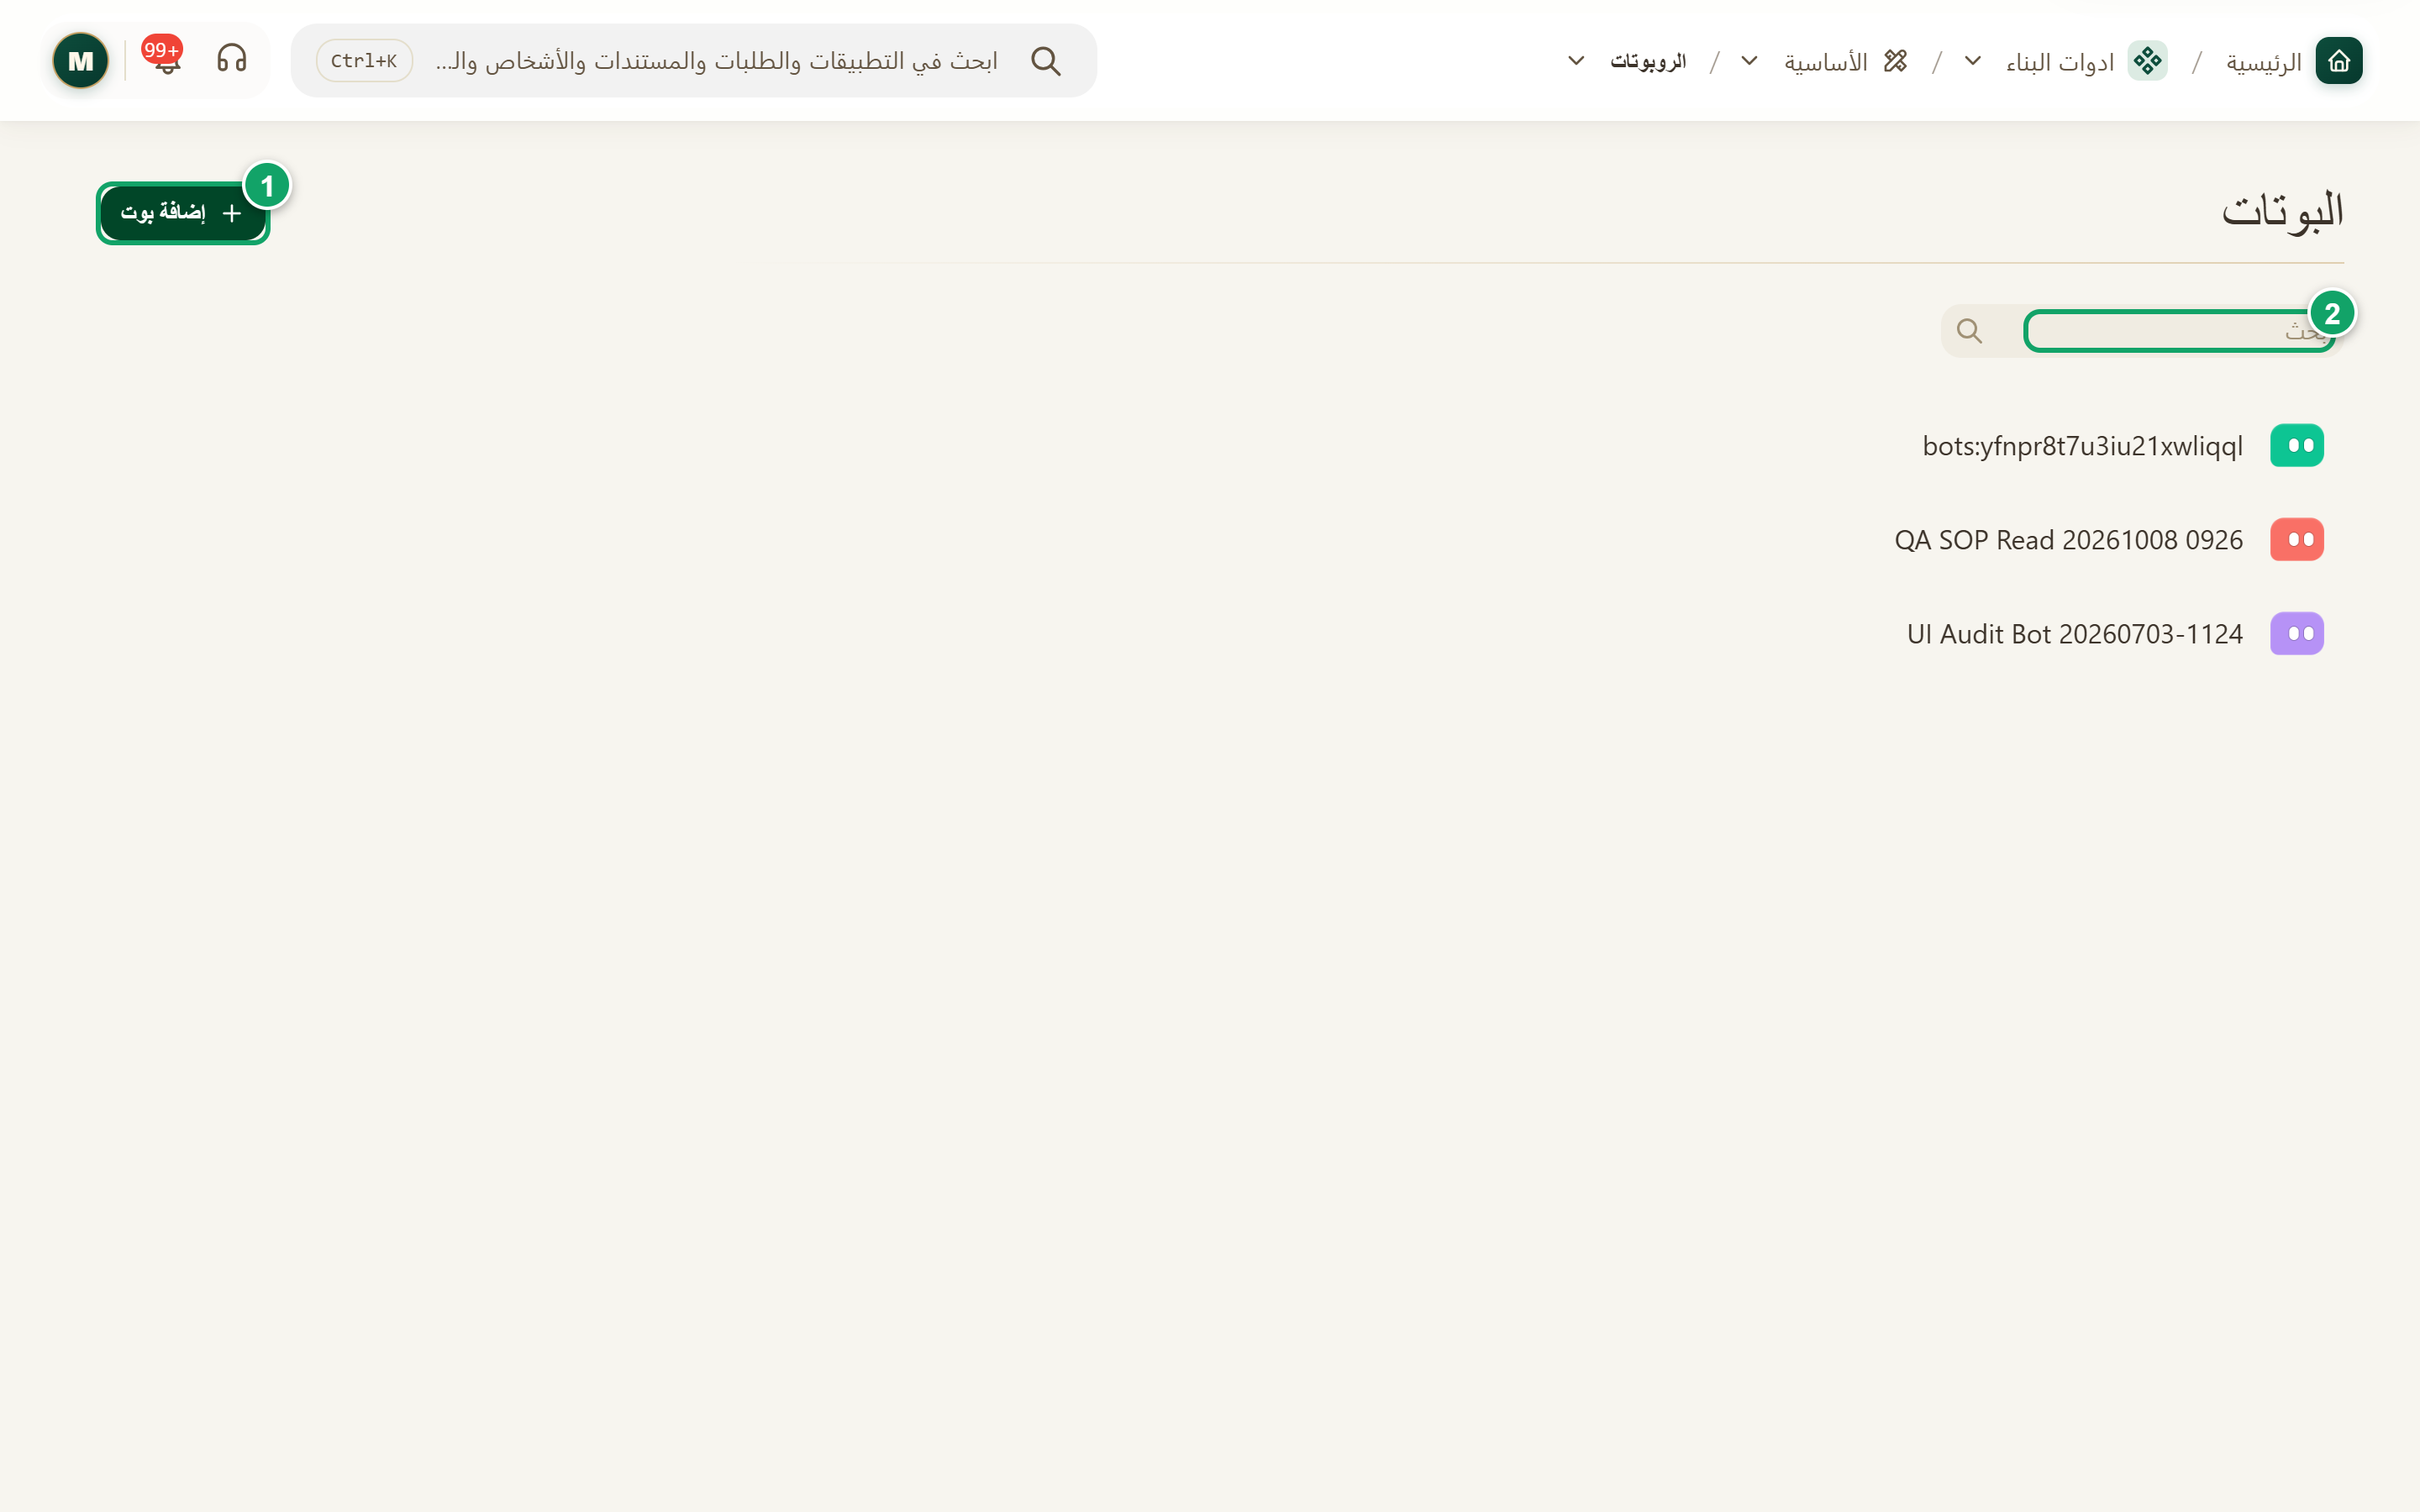
\includegraphics[width=0.95\linewidth,height=0.72\textheight,keepaspectratio]{figures/screens/ch06-bots-ar.png}
\caption{صفحة «البوتات»}
\label{fig:builder-bots-screen}
\shotnote{تعرض الصفحة البوتات المعرّفة في المؤسسة، وهي هنا بوتات اختبار. ① «إضافة بوت»: يطلب الاسم فقط. ② البحث: يجد البوت بالاسم.}
\end{figure}


\begin{table}[H]
\centering
\caption{إعدادات البوت}
\label{tab:builder-bots-data}
\begin{tabularx}{\linewidth}{R{3.6cm} Y}
\rcHeaderRow
\thh{القسم} & \thh{ماذا تحدد؟}\\
إضافة بوت & يطلب الاسم فقط، وتُختار صورته تلقائياً.\\
الدردشة & هل يُضاف إلى الدردشات المباشرة أو القنوات، وهل يمكن مراسلته أو ذكره.\\
البريد الإلكتروني & هل يُثبّت في البريد، وهل يمكن إضافته في نسخة، وإضافة جهات اتصال داخلية أو خارجية.\\
التقويم & هل يمكن تثبيته في التقويم.\\
التثبيت الافتراضي & هل يُضاف تلقائياً إلى الدردشة أو البريد أو التقويم، وحدود وصوله الافتراضية إلى البريد.\\
\end{tabularx}
\end{table}

\begin{figure}[H]
\centering
\begin{tikzpicture}[node distance=0.5cm]
\node[entity] (bot) {\RL{البوت}};
\node[entityOpt,below right=0.7cm and 0.3cm of bot] (where) {\RL{أين يُضاف}};
\node[entityOpt,below left=0.7cm and 0.3cm of bot] (sop) {\RL{إجراء داخلي يرد}};
\draw[dependsOnOpt] (bot.south) -- ++(0,-0.3) -| (where.north);
\draw[dependsOnOpt] (bot.south) -- ++(0,-0.3) -| (sop.north);
\end{tikzpicture}
\rclegend
\caption{هوية البوت وعمله}
\label{fig:builder-bots-model}
\shotnote{يفصل الشكل بين أمرين: هذه الصفحة تحدد هوية البوت وأماكن إضافته، أما ردوده فيبنيها إجراء داخلي يبدأ عندما يُراسَل البوت أو يُذكر. لذلك لا يفعل البوت شيئاً وحده حتى تربطه بإجراء منشور.}
\end{figure}

\subsection{خطوات العمل والتحقق}
\begin{enumerate}
\item افتح «البوتات» واضغط «إضافة بوت»، ثم اكتب الاسم واضغط «إنشاء».
\item افتح البوت، وفعّل أماكن إضافته في الدردشة والبريد والتقويم، ثم اضغط «حفظ».
\item ابنِ في «الإجراءات الداخلية» إجراءً يبدأ «عند رسالة مباشرة إلى الروبوت» وانشره.
\end{enumerate}

\textbf{تحقق ومعالجة المشكلة:} أضف البوت إلى دردشة تجريبية وأرسل إليه رسالة، فيجب أن يبدأ الإجراء ويظهر في «عمليات التشغيل». فإذا لم تظهر خيارات الإضافة للأعضاء، فراجع إعدادات الدردشة والحفظ؛ وإذا لم يرد البوت، فتأكد من أن الإجراء منشور وغير متوقف.

\clearpage
\section{قوالب DOCX}
\label{sec:builder-feature-docx-templates}

قالب DOCX ملف Word عادي تكتب فيه النص الثابت، وتضع مكان البيانات المتغيرة وسوماً بين قوسين مزدوجين، مثل اسم الموظف أو رقم الطلب. وعندما يضغط المستخدم زر الإجراء في السجل، يملأ كيان الوسوم من بيانات السجل وينزّل المستند بصيغة Word أو PDF. وبذلك تُنشئ العقود والخطابات بنص موحّد دون نسخ يدوي.

\textbf{المسار ومن يستخدمه:} «ادوات البناء» ← «الأساسية» ← «قوالب DOCX». يديرها من يملك إدارة أدوات البناء، أما المستخدمون فيستعملونها من زر في السجل.

\begin{rcnote}[مثال: شركة الأفق]
يكتب مسؤول النظام خطاب تأكيد الزيارة في Word، ويضع وسماً لرقم الطلب وآخر لموعد الزيارة، ثم يرفعه قالباً ويربطه بزر في «طلبات الزيارة». ويرفع الخطاب من ① ويختبره بعد فتحه من ③.
\end{rcnote}

\begin{figure}[H]
\centering
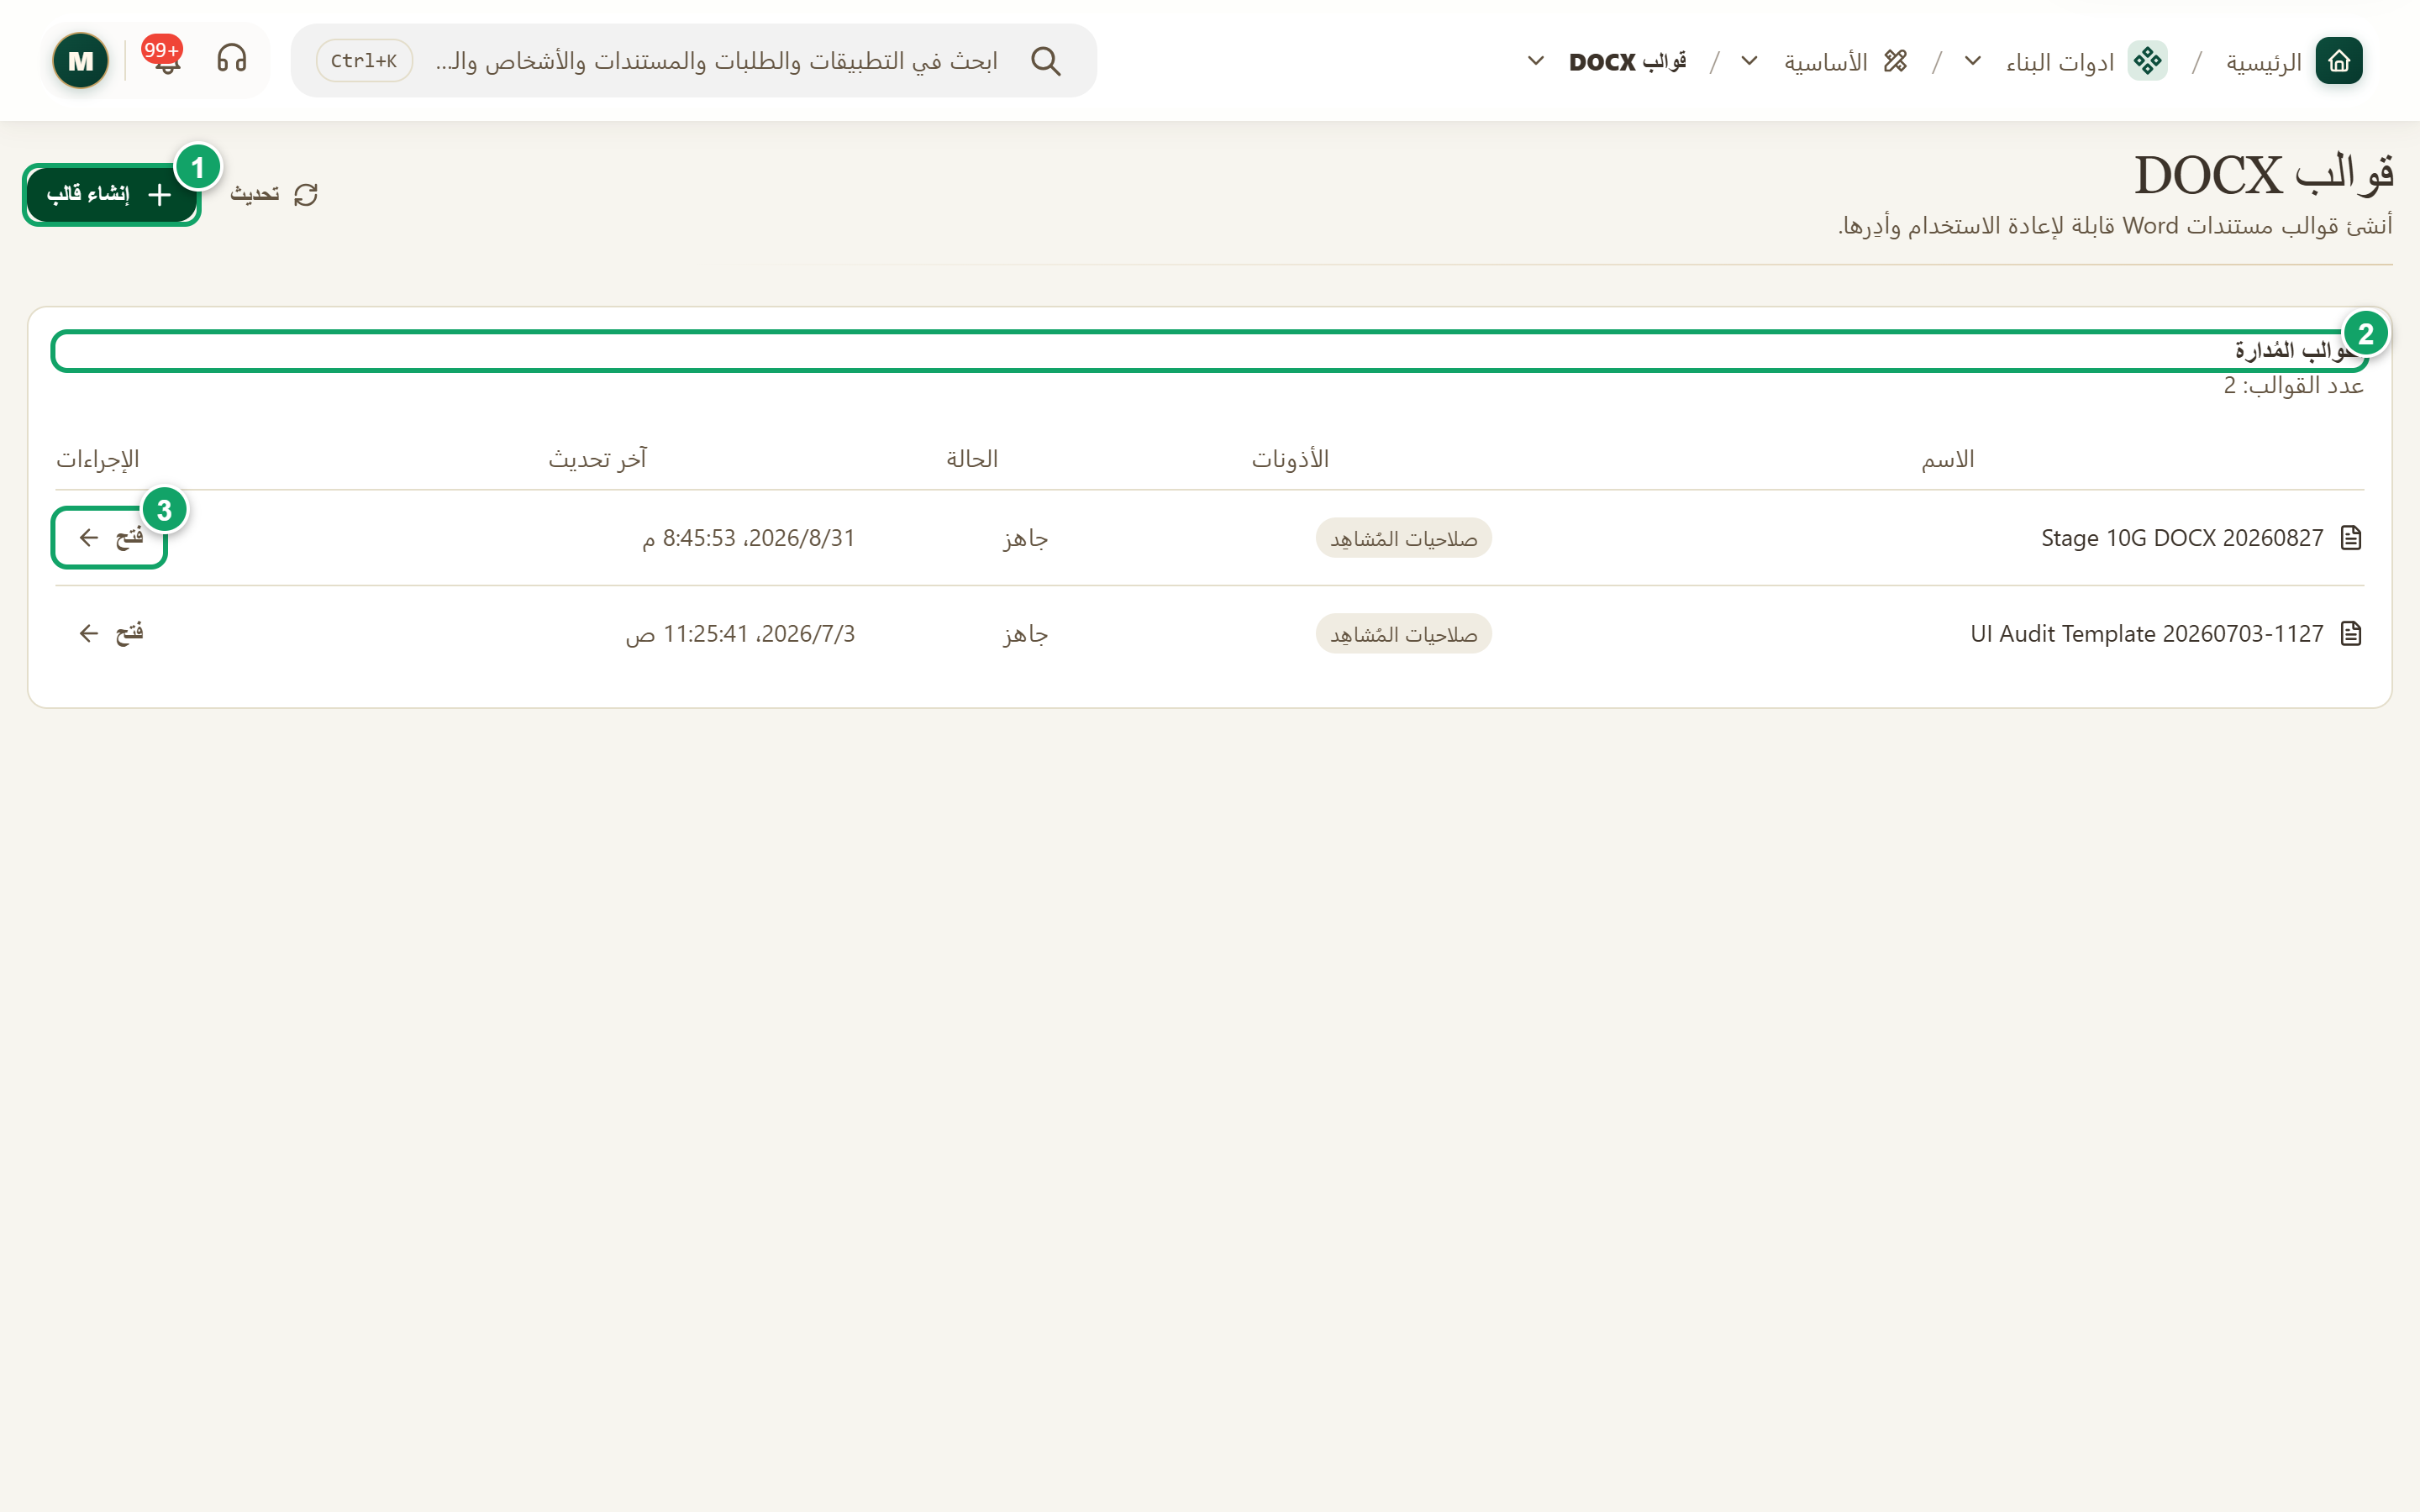
\includegraphics[width=0.95\linewidth,height=0.72\textheight,keepaspectratio]{figures/screens/ch06-docx-ar.png}
\caption{صفحة «قوالب DOCX»}
\label{fig:builder-docx-templates-screen}
\shotnote{تعرض الصفحة القوالب المُدارة وأذوناتها وحالاتها، وهي هنا قوالب اختبار. ① «إنشاء قالب»: يرفع ملف Word جديداً. ② «القوالب المُدارة»: القائمة مع حالة كل قالب. ③ «فتح»: يفتح القالب للإعدادات والإصدارات والاختبار.}
\end{figure}


\begin{table}[H]
\centering
\caption{ما الذي تجده هنا؟}
\label{tab:builder-docx-data}
\begin{tabularx}{\linewidth}{R{3.6cm} Y}
\rcHeaderRow
\thh{الجزء} & \thh{المحتوى والإجراء}\\
القوالب المُدارة & قائمة القوالب مع «الأذونات» و«الحالة»: «جاهز» عندما يوجد إصدار حالي، أو «يحتاج إلى مستند Word».\\
إنشاء قالب & ترفع «مستند Word» وتكتب «اسم القالب»، ويمكنك ضبط اسم الملف المنزَّل وأذونات المستند.\\
أذونات المستند & «صلاحيات المُشاهِد»، وهي الموصى بها، تعرض فقط ما يستطيع من ينزّل الملف رؤيته. أما «صلاحيات المسؤول» فقد تضع في المستند بيانات لا يراها.\\
الإعدادات والإصدارات & عدّل الإعدادات، وارفع إصداراً جديداً بعد التحقق منه، وراجع «سجل الإصدارات».\\
اختبار وتحميل & اختر سجلاً حقيقياً وصيغة Word أو PDF، ثم «إنشاء وتنزيل» لترى النتيجة قبل أن يستخدمها أحد.\\
\end{tabularx}
\end{table}

\begin{table}[H]
\centering
\caption{أمثلة على الوسوم}
\label{tab:builder-docx-tags}
\begin{tabularx}{\linewidth}{R{3.6cm} Y}
\rcHeaderRow
\thh{الوسم} & \thh{ماذا يفعل؟}\\
\en{\{\{ \$record.field\_key \}\}} & يضع قيمة حقل من السجل، باستخدام مفتاح الحقل لا تسميته.\\
\en{\{\{\#if ...\}\}} & يُظهر فقرة عندما يتحقق شرط، وينتهي بـ \en{\{\{/if\}\}}.\\
\en{\{\{\#each ...\}\}} & يكرر صفاً أو فقرة لكل عنصر في قائمة، وينتهي بـ \en{\{\{/each\}\}}.\\
\end{tabularx}
\end{table}

\begin{figure}[H]
\centering
\begin{tikzpicture}[node distance=0.5cm]
\node[stepBox] (a) {\RL{ملف Word بوسوم}};
\node[stepBox,below=of a] (b) {\RL{إنشاء قالب واختباره}};
\node[stepBox,below=of b] (c) {\RL{إجراء «مستند Word» في السجل}};
\node[stepBox,below=of c] (d) {\RL{المستخدم يضغط الزر}};
\draw[flowsTo] (a) -- (b);
\draw[flowsTo] (b) -- (c);
\draw[flowsTo] (c) -- (d);
\end{tikzpicture}
\rclegend
\caption{من ملف Word إلى مستند لكل سجل}
\label{fig:builder-docx-flow}
\shotnote{يبيّن المخطط أن القالب لا يرتبط بنوع سجلات بنفسه، بل يصل إلى المستخدم عبر إجراء من نوع «مستند Word» تضيفه في «الإجراءات والأتمتة». لذلك يأتي الاختبار على سجل حقيقي قبل الربط، لأن التحقق عند الرفع لا يكشف كل خطأ في موضع الوسوم.}
\end{figure}

\subsection{خطوات العمل والتحقق}
\begin{enumerate}
\item اكتب المستند في Word، وضع الوسوم بمفاتيح الحقول الفعلية، واجعل وسوم الشرط والتكرار في فقرة مستقلة.
\item افتح «قوالب DOCX» واضغط «إنشاء قالب»، ثم ارفع الملف واكتب الاسم واضغط «إنشاء قالب».
\item افتح «اختبار وتحميل»، واختر سجلاً، ثم «إنشاء وتنزيل» وراجع المستند.
\item أضف في نوع السجلات إجراءً من نوع «مستند Word» واربطه بالقالب، ثم انشر.
\end{enumerate}

\textbf{تحقق ومعالجة المشكلة:} يجب أن تظهر حالة القالب «جاهز»، وأن ينزّل زر الإجراء مستنداً ممتلئاً ببيانات السجل. فإذا ظهر «هذا المستند يحتاج إلى مراجعة» عند الرفع، فصحّح الوسوم المذكورة وأعد الرفع. وإذا ظهرت قيمة فارغة، فتأكد من أنك استخدمت مفتاح الحقل لا تسميته.

\clearpage
\section{قوالب XLSX}
\label{sec:builder-feature-xlsx-templates}

قالب XLSX مصنف Excel فيه وسوم بالطريقة نفسها، يملؤه كيان من بيانات السجل وينزّله بصيغة Excel أو PDF. ويناسب الكشوف والتقارير الجدولية التي تتكرر صفوفها، لأن الوسوم تستطيع تكرار الصفوف والأعمدة. ويحافظ الوسم الموضوع وحده في خلية على نوع القيمة رقماً أو تاريخاً.

\textbf{المسار ومن يستخدمه:} «ادوات البناء» ← «الأساسية» ← «قوالب XLSX». يديرها من يملك إدارة أدوات البناء.

\begin{rcnote}[مثال: شركة الأفق]
يجهّز مسؤول النظام مصنف «كشف زيارات الفرع» يكرر صفاً لكل زيارة، ويربطه بزر من نوع «جدول بيانات»، فتنزّل سارة الخطيب الكشف جاهزاً بصيغة Excel. ويرفع المصنف من ①.
\end{rcnote}

\begin{figure}[H]
\centering
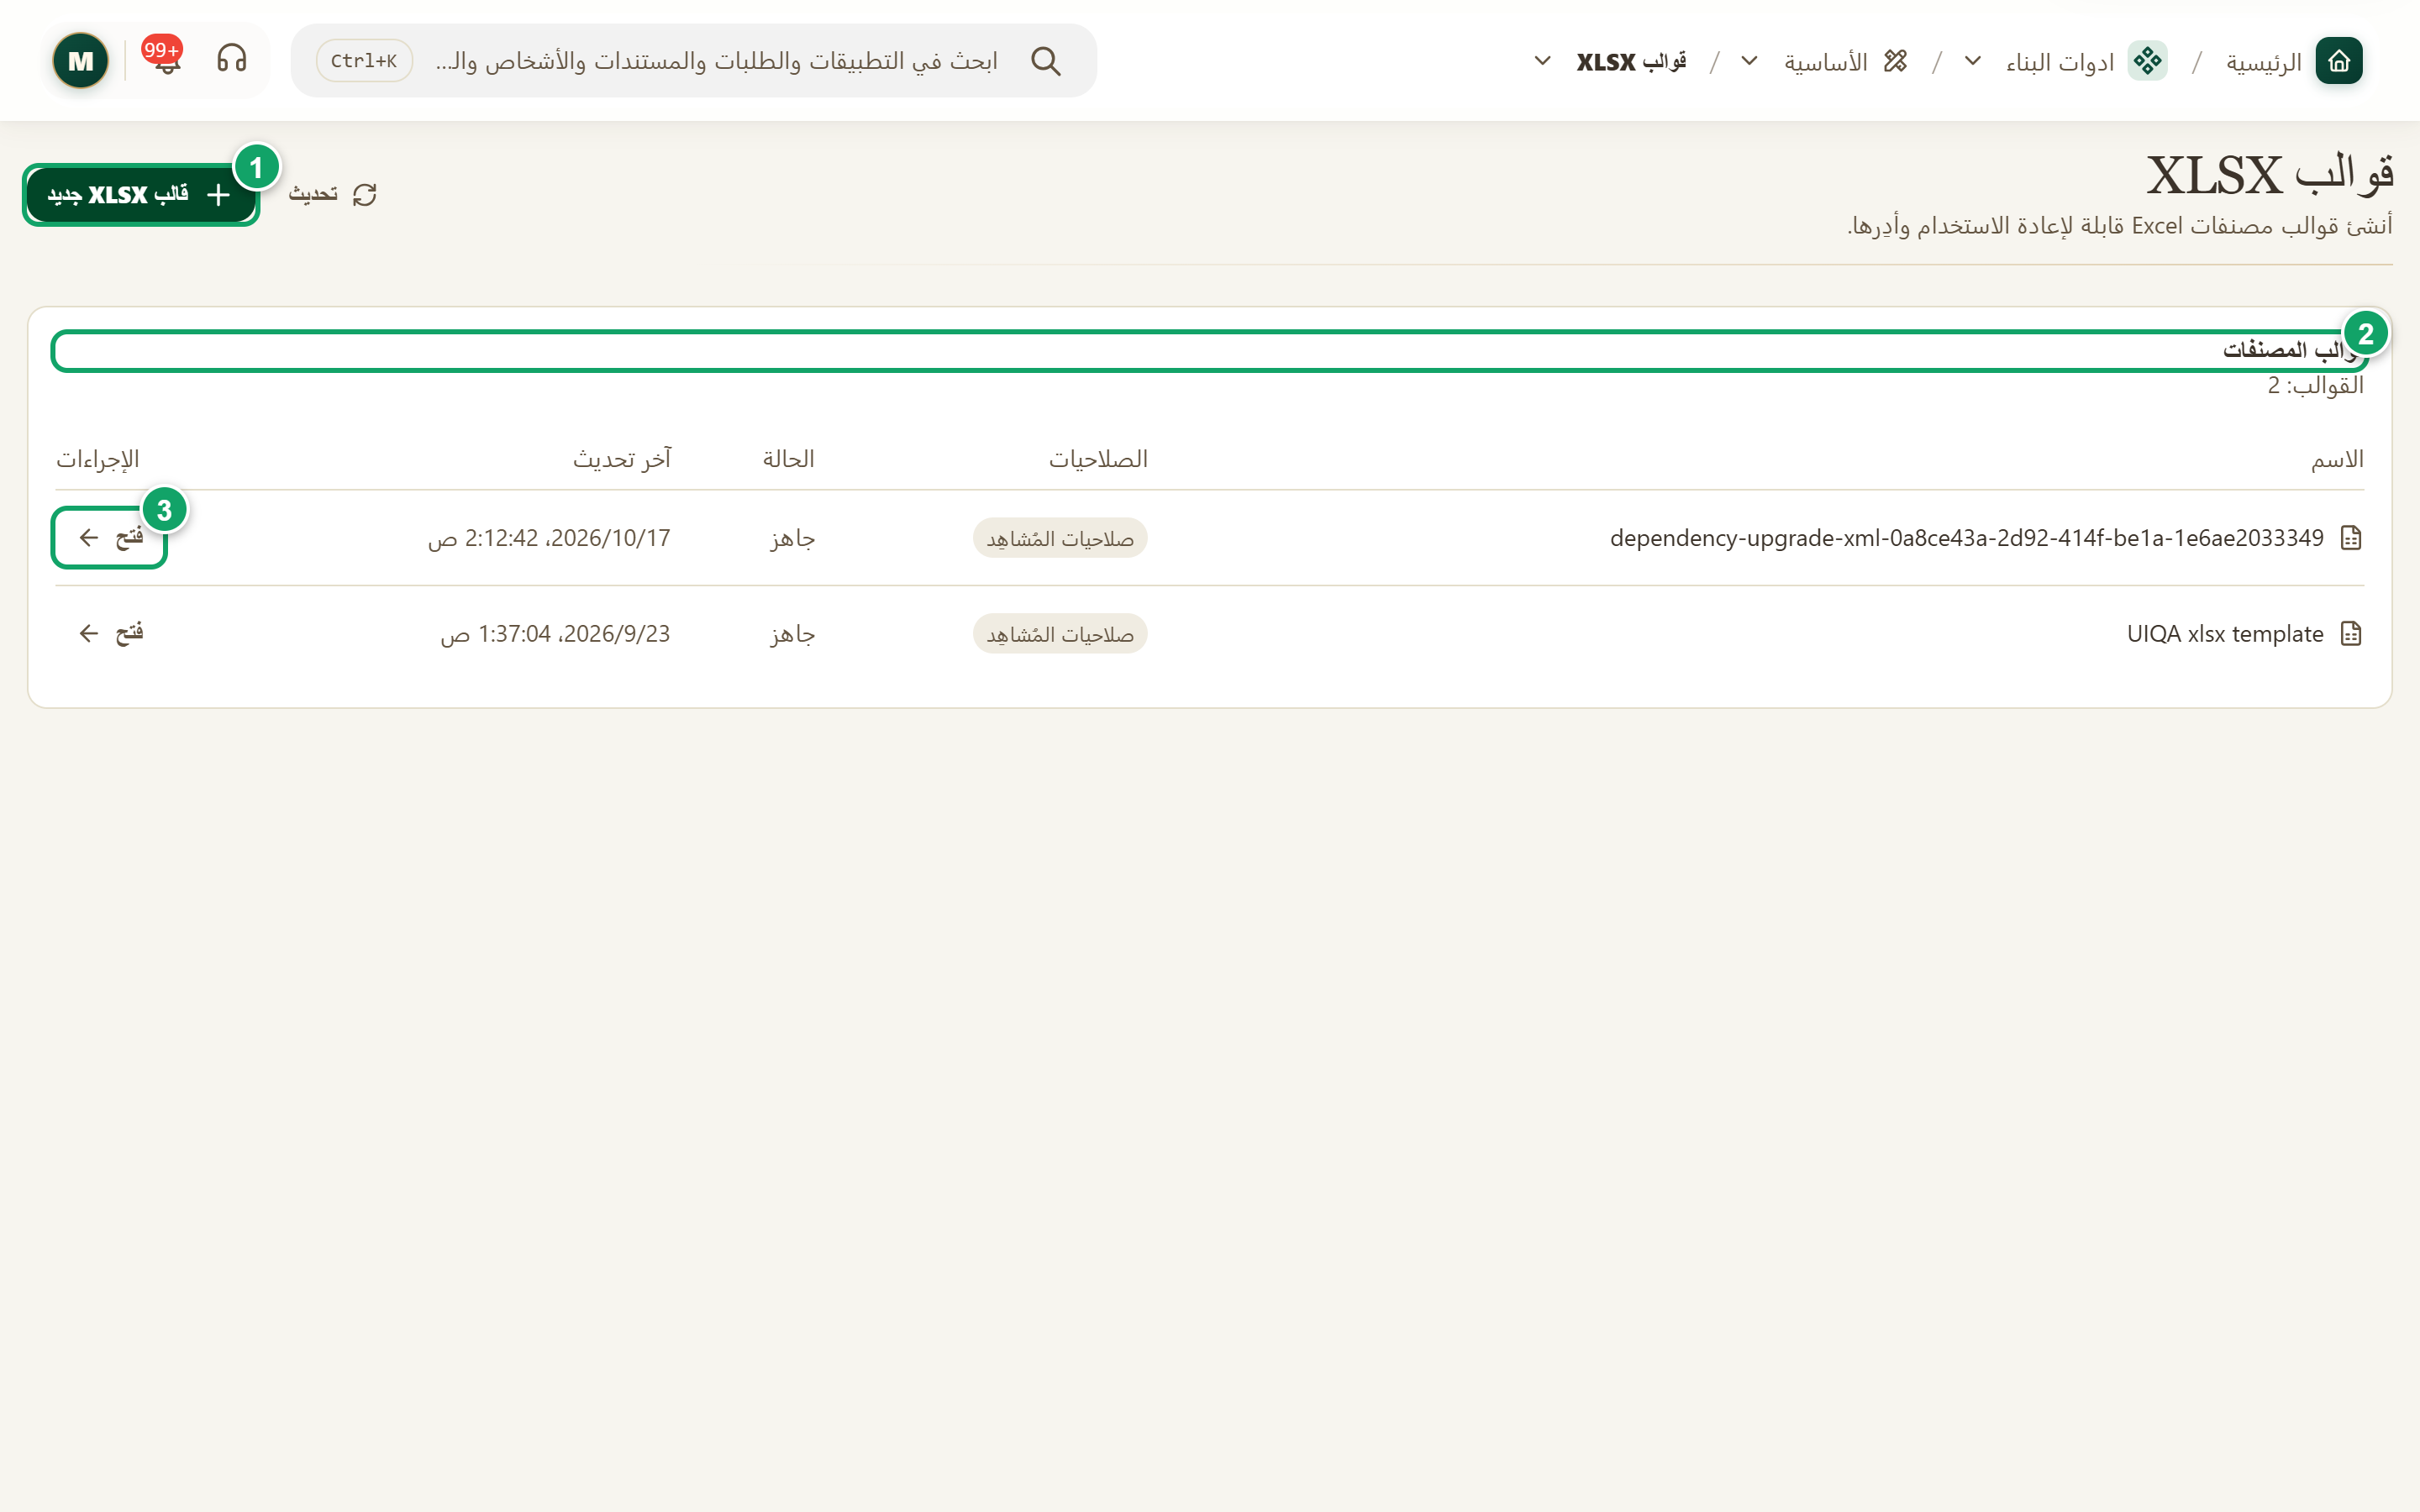
\includegraphics[width=0.95\linewidth,height=0.72\textheight,keepaspectratio]{figures/screens/ch06-xlsx-ar.png}
\caption{صفحة «قوالب XLSX»}
\label{fig:builder-xlsx-templates-screen}
\shotnote{تعرض الصفحة قوالب المصنفات وحالاتها، وهي هنا قوالب اختبار. ① «قالب XLSX جديد»: يرفع مصنف Excel. ② «قوالب المصنفات»: القائمة مع الحالة. ③ «فتح»: يفتح القالب لاختباره.}
\end{figure}


\begin{table}[H]
\centering
\caption{ما الذي تجده هنا؟}
\label{tab:builder-xlsx-data}
\begin{tabularx}{\linewidth}{R{3.6cm} Y}
\rcHeaderRow
\thh{الجزء} & \thh{المحتوى والإجراء}\\
قوالب المصنفات & قائمة القوالب وحالتها: «جاهز» أو «يحتاج إلى مصنف Excel».\\
قالب XLSX جديد & ترفع «مصنف Excel» وتكتب «اسم القالب»، ويمكنك ضبط «صيغة اسم الملف عند التنزيل» و«أذونات البيانات».\\
الإصدارات & استبدال المصنف بإصدار جديد ومراجعة الإصدارات السابقة.\\
اختبار وتحميل & تجربة القالب ببيانات، ثم «إنشاء XLSX» أو «إنشاء PDF».\\
الوسوم الخاصة بـExcel & تكرار الصفوف بـ \en{\{\{\#each\}\}}، وتكرار الأعمدة بـ \en{\{\{\#eachCol\}\}}، وإخفاء صف أو عمود عند الحاجة.\\
\end{tabularx}
\end{table}

\begin{figure}[H]
\centering
\begin{tikzpicture}[node distance=0.5cm]
\node[entity] (tpl) {\RL{قالب XLSX}};
\node[entityOpt,below right=0.7cm and 0.3cm of tpl] (xlsx) {\RL{ملف Excel}};
\node[entityOpt,below left=0.7cm and 0.3cm of tpl] (pdf) {\RL{ملف PDF}};
\draw[dependsOnOpt] (tpl.south) -- ++(0,-0.3) -| (xlsx.north);
\draw[dependsOnOpt] (tpl.south) -- ++(0,-0.3) -| (pdf.north);
\end{tikzpicture}
\rclegend
\caption{صيغتا الإخراج}
\label{fig:builder-xlsx-outputs}
\shotnote{يوضّح الشكل أن القالب الواحد يُخرج ملف Excel أو PDF، وتختار ما يُسمح به عند ربطه بالإجراء عبر «السماح بملفات PDF». فاستخدم Excel عندما يحتاج المستلم إلى معالجة الأرقام، وPDF عندما تريد نسخة ثابتة للعرض أو الأرشيف.}
\end{figure}

\subsection{خطوات العمل والتحقق}
\begin{enumerate}
\item جهّز المصنف في Excel، وضع الوسوم في الخلايا المناسبة.
\item افتح «قوالب XLSX» واضغط «قالب XLSX جديد»، ثم ارفع المصنف واكتب الاسم واضغط «إنشاء قالب».
\item جرّب القالب من «اختبار وتحميل»، ثم أضف إجراءً من نوع «جدول بيانات» في نوع السجلات واربطه بالقالب.
\end{enumerate}

\textbf{تحقق ومعالجة المشكلة:} يجب أن تظهر حالة القالب «جاهز»، وأن يتكرر الصف لكل عنصر في الملف الناتج. فإذا ظهر رقم نصاً، فاجعل الوسم وحده في خليته. وإذا تعذّر عليك إنشاء القالب، فإدارة القوالب تحتاج إلى صلاحية إدارة أدوات البناء لا إلى مقعد كامل فقط.

\clearpage
\section{قوالب الطباعة}
\label{sec:builder-feature-print-templates}

قالب الطباعة مستند تصممه داخل كيان بالسحب والإفلات، دون أن ترفع ملف Word. ويطبع طلبات نموذج أو سجلات نوع معين بصيغة PDF أو Word، على ترويسة المؤسسة وهويتها. وتعرض صفحة «قوالب الطباعة» كل القوالب الموجودة وحالتها، أما إنشاء قالب جديد فيتم من داخل منشئ النموذج أو نوع السجلات بالضغط على «طباعة».

\textbf{المسار ومن يستخدمه:} «ادوات البناء» ← «الأساسية» ← «قوالب الطباعة». يستخدمها من يبني النماذج وأنواع السجلات.

\begin{rcnote}[مثال: شركة الأفق]
يفتح مسؤول النظام نوع «طلبات الزيارة» ويضغط «طباعة»، ثم يختار «ابدأ من نوع السجل هذا» ليصمم ورقة زيارة فيها رمز QR للتحقق، وينشرها فتظهر في زر «طباعة» داخل كل طلب. ويصل إلى القالب من ③.
\end{rcnote}

\begin{figure}[H]
\centering
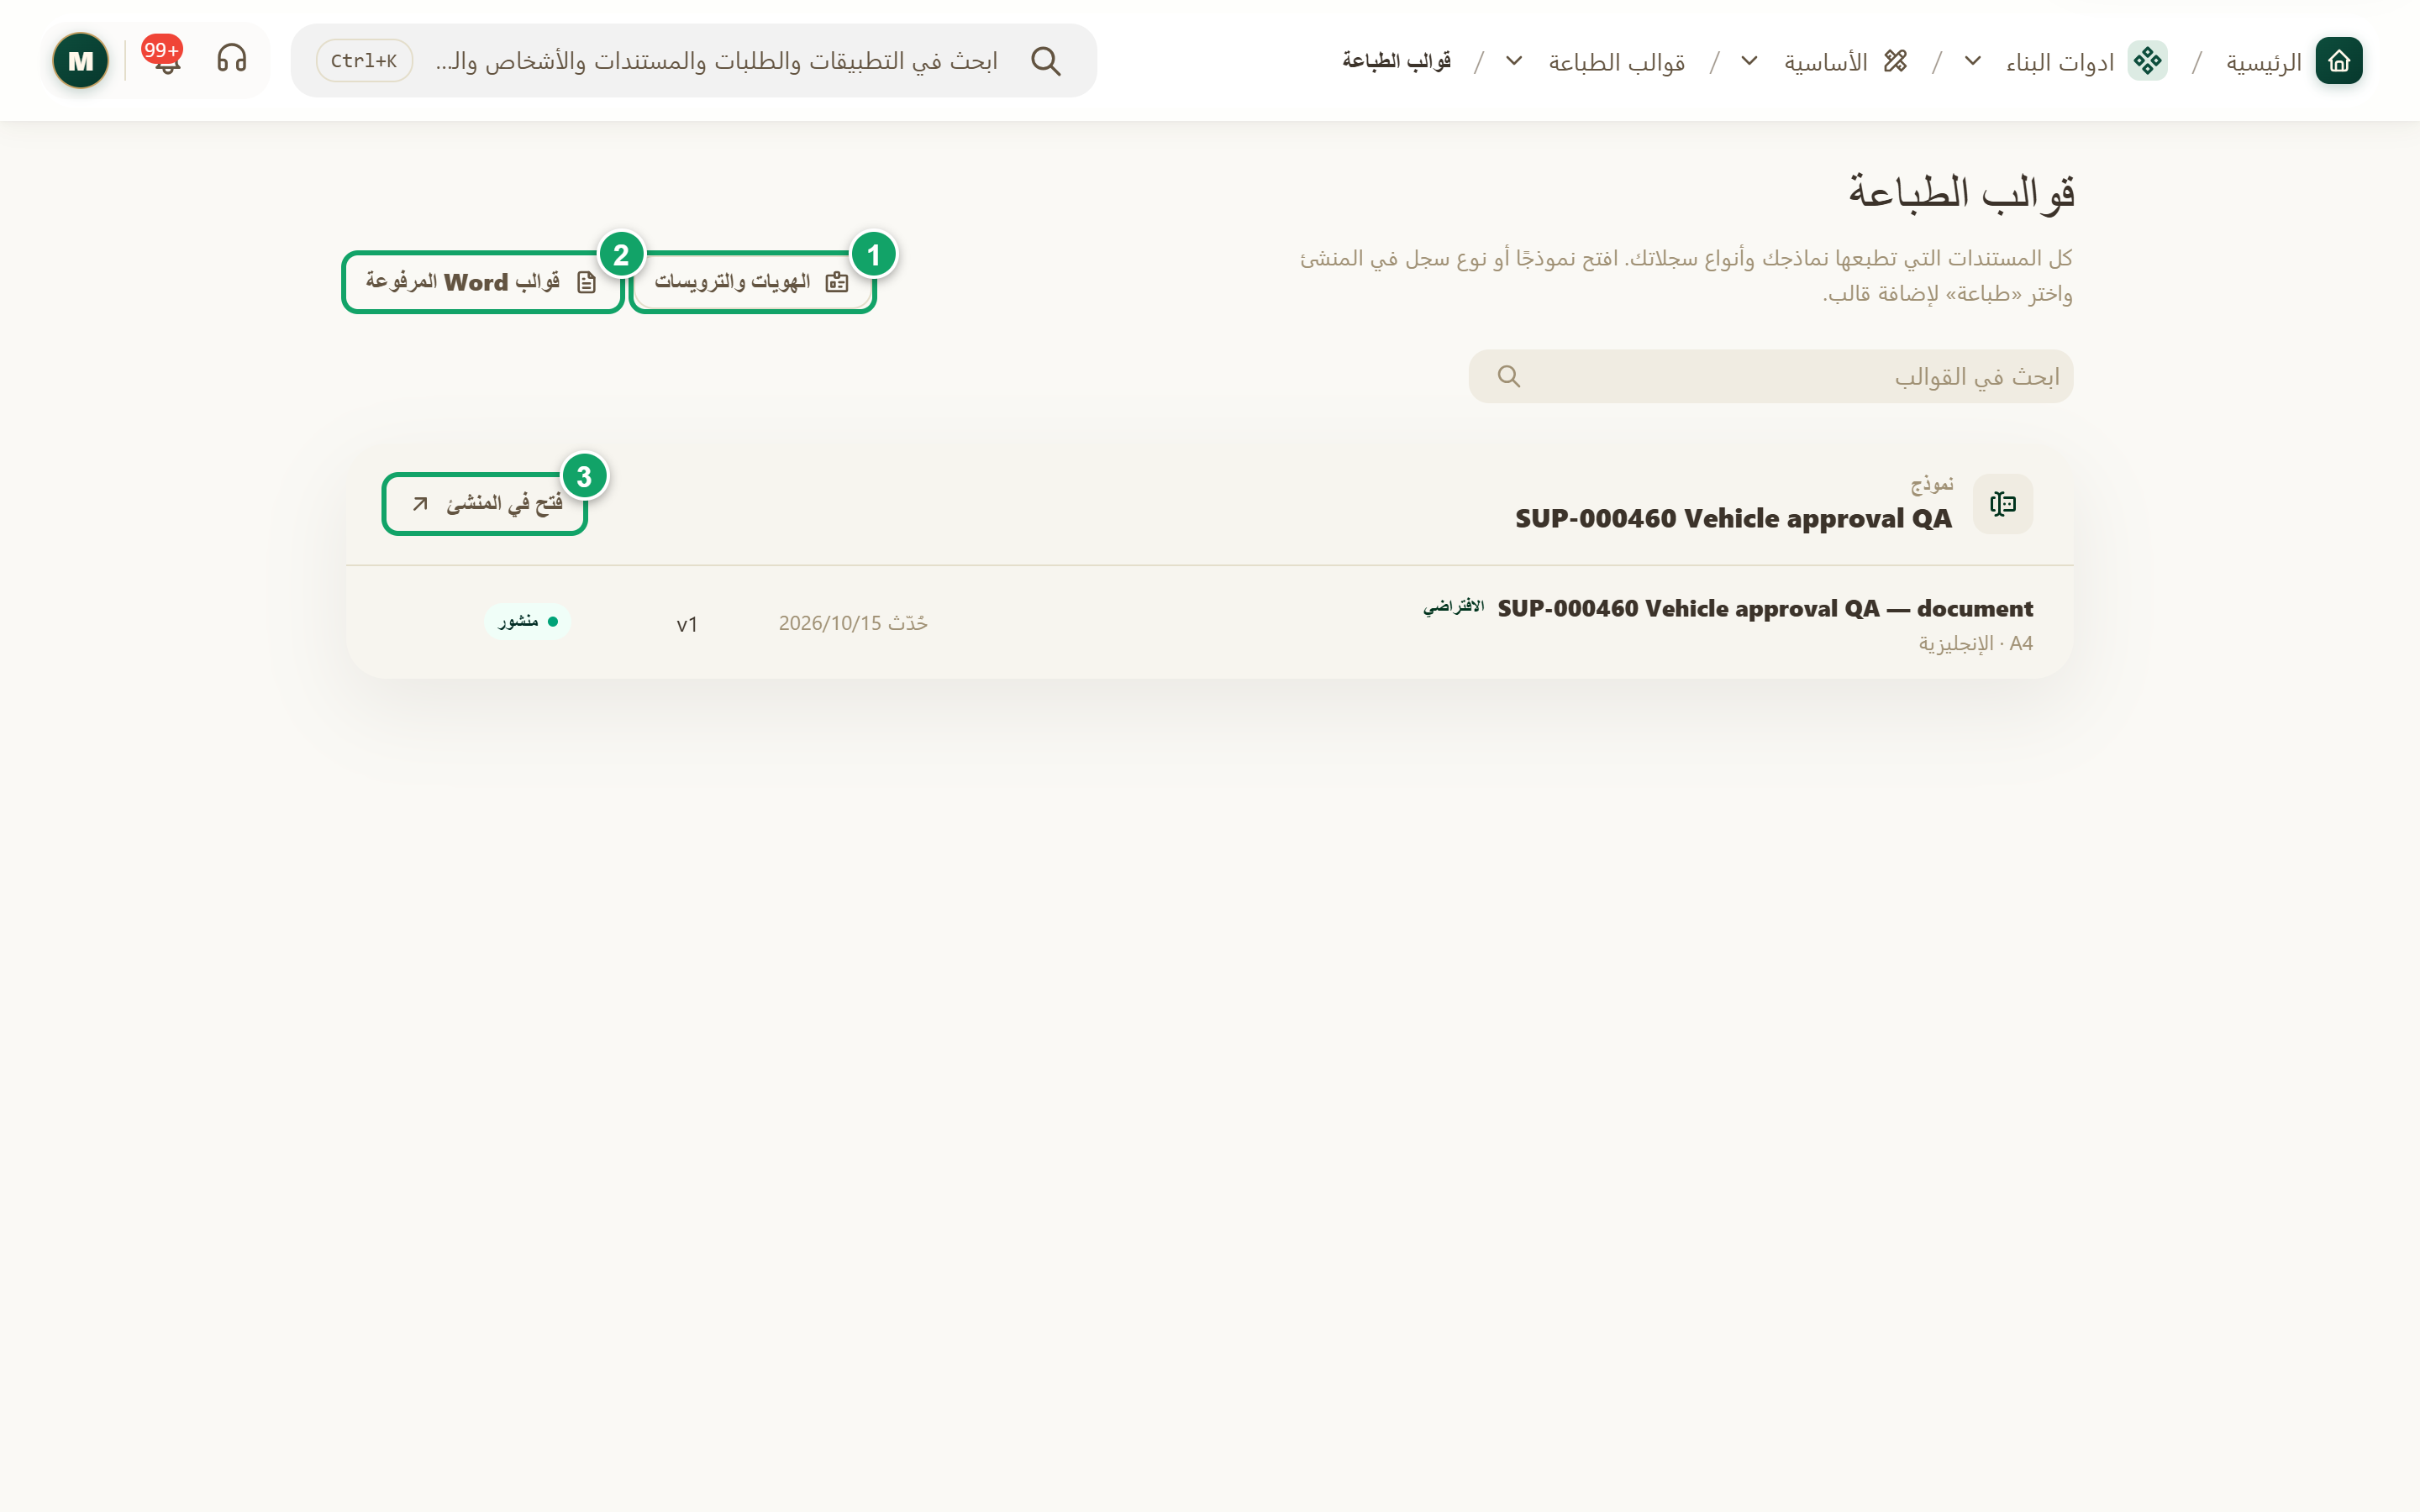
\includegraphics[width=0.95\linewidth,height=0.72\textheight,keepaspectratio]{figures/screens/ch06-print-ar.png}
\caption{مكتبة «قوالب الطباعة»}
\label{fig:builder-print-templates-screen}
\shotnote{تعرض الصفحة قوالب الطباعة مجمّعة حسب النموذج أو نوع السجلات، مع حالتها. والقالب الظاهر قالب اختبار. ① «الهويات والترويسات»: ينتقل إلى الشعارات والترويسات. ② «قوالب Word المرفوعة»: ينتقل إلى قوالب DOCX. ③ «فتح في المنشئ»: يفتح النموذج أو النوع حيث يُعدَّل القالب.}
\end{figure}


\begin{table}[H]
\centering
\caption{ما الذي تجده هنا؟}
\label{tab:builder-print-data}
\begin{tabularx}{\linewidth}{R{3.6cm} Y}
\rcHeaderRow
\thh{الجزء} & \thh{المحتوى والإجراء}\\
مكتبة القوالب & القوالب مجمّعة حسب النموذج أو نوع السجل، مع الحجم واللغة والإصدار والحالة: «منشور» أو «مسودة» أو «تغييرات غير منشورة»، وزر «فتح في المنشئ».\\
قالب جديد & من نافذة «طباعة» في المنشئ: «ابدأ من هذا النموذج» أو «ابدأ من نوع السجل هذا» أو «صفحة فارغة على ترويسة الجهة».\\
المحرر & تبويب «البيانات» للحقول، و«العناصر» مثل النص والجدول والصورة والشعار ورمز QR والتوقيع ومسار الموافقة، و«الصفحة» للورق والهوامش والهوية والترويسة.\\
المخرجات & الصيغ المتاحة للتنزيل، واسم الملف، و«من يمكنه الطباعة»، والاحتفاظ بنسخة في السجل، وصفحة تحقق يفتحها رمز QR.\\
\end{tabularx}
\end{table}

\begin{figure}[H]
\centering
\begin{tikzpicture}[node distance=0.5cm]
\node[stepBox] (a) {\RL{طباعة من منشئ النموذج أو النوع}};
\node[stepBox,below=of a] (b) {\RL{تصميم البيانات والعناصر}};
\node[stepBox,below=of b] (c) {\RL{معاينة بسجل}};
\node[stepBox,below=of c] (d) {\RL{نشر}};
\node[stepBox,below=of d] (e) {\RL{زر طباعة في السجل}};
\draw[flowsTo] (a) -- (b);
\draw[flowsTo] (b) -- (c);
\draw[flowsTo] (c) -- (d);
\draw[flowsTo] (d) -- (e);
\end{tikzpicture}
\rclegend
\caption{من التصميم إلى زر الطباعة}
\label{fig:builder-print-flow}
\shotnote{يبيّن المخطط أن القالب يولد داخل منشئ النموذج أو نوع السجلات، لا في صفحة المكتبة، وأنه لا يظهر للمستخدمين قبل النشر. وتأتي المعاينة بسجل حقيقي قبل النشر لتكشف الحقول الفارغة أو الجداول الطويلة قبل أن يطبعها أحد.}
\end{figure}

\subsection{خطوات العمل والتحقق}
\begin{enumerate}
\item افتح النموذج أو نوع السجلات في المنشئ، واضغط «طباعة»، ثم اختر نقطة البداية.
\item أضف الحقول والعناصر، واضبط في «الصفحة» الورق والهوية والترويسة.
\item اضغط «معاينة بسجل» و«تنزيل ملف PDF تجريبي»، ثم حدد «من يمكنه الطباعة» واضغط «نشر».
\end{enumerate}

\textbf{تحقق ومعالجة المشكلة:} يجب أن يظهر القالب «منشور» في المكتبة، وأن يظهر في قائمة «اختر مستندًا» عند الضغط على «طباعة» في السجل. فإذا لم يظهر، فتأكد من نشره، لأن القالب «لا يظهر قبل النشر»؛ واستخدم «الفحص على جميع السجلات» لاكتشاف السجلات التي تنقصها بيانات.

\clearpage
\section{الهويات والترويسات}
\label{sec:builder-feature-identities}

الهوية هي شعار المؤسسة واسمها وألوانها وبياناتها الرسمية، مثل السجل التجاري والعنوان. أما الترويسة فرأس الصفحة وتذييلها اللذان يظهران في المستندات المطبوعة. وتحفظهما هذه الصفحة في مكان واحد، فتستخدمهما قوالب الطباعة والمراسلات الرسمية معاً، وأي تغيير هنا يظهر فيها كلها في الطباعة التالية.

\textbf{المسار ومن يستخدمه:} «ادوات البناء» ← «الأساسية» ← «الهويات والترويسات». يستخدمها من يدير مظهر مستندات المؤسسة.

\begin{rcnote}[مثال: شركة الأفق]
يرفع مسؤول النظام شعار الأفق ويضيف بياناتها الرسمية إلى الهوية الافتراضية، ثم ينشئ ترويسة يظهر رأسها في الصفحة الأولى فقط، فتطبع ورقة الزيارة بشعار الشركة دون إعادة تصميمه في كل قالب. ويرفع الشعار في ③ ويحفظ من ④، ثم ينشئ الترويسة من ②.
\end{rcnote}

\begin{figure}[H]
\centering
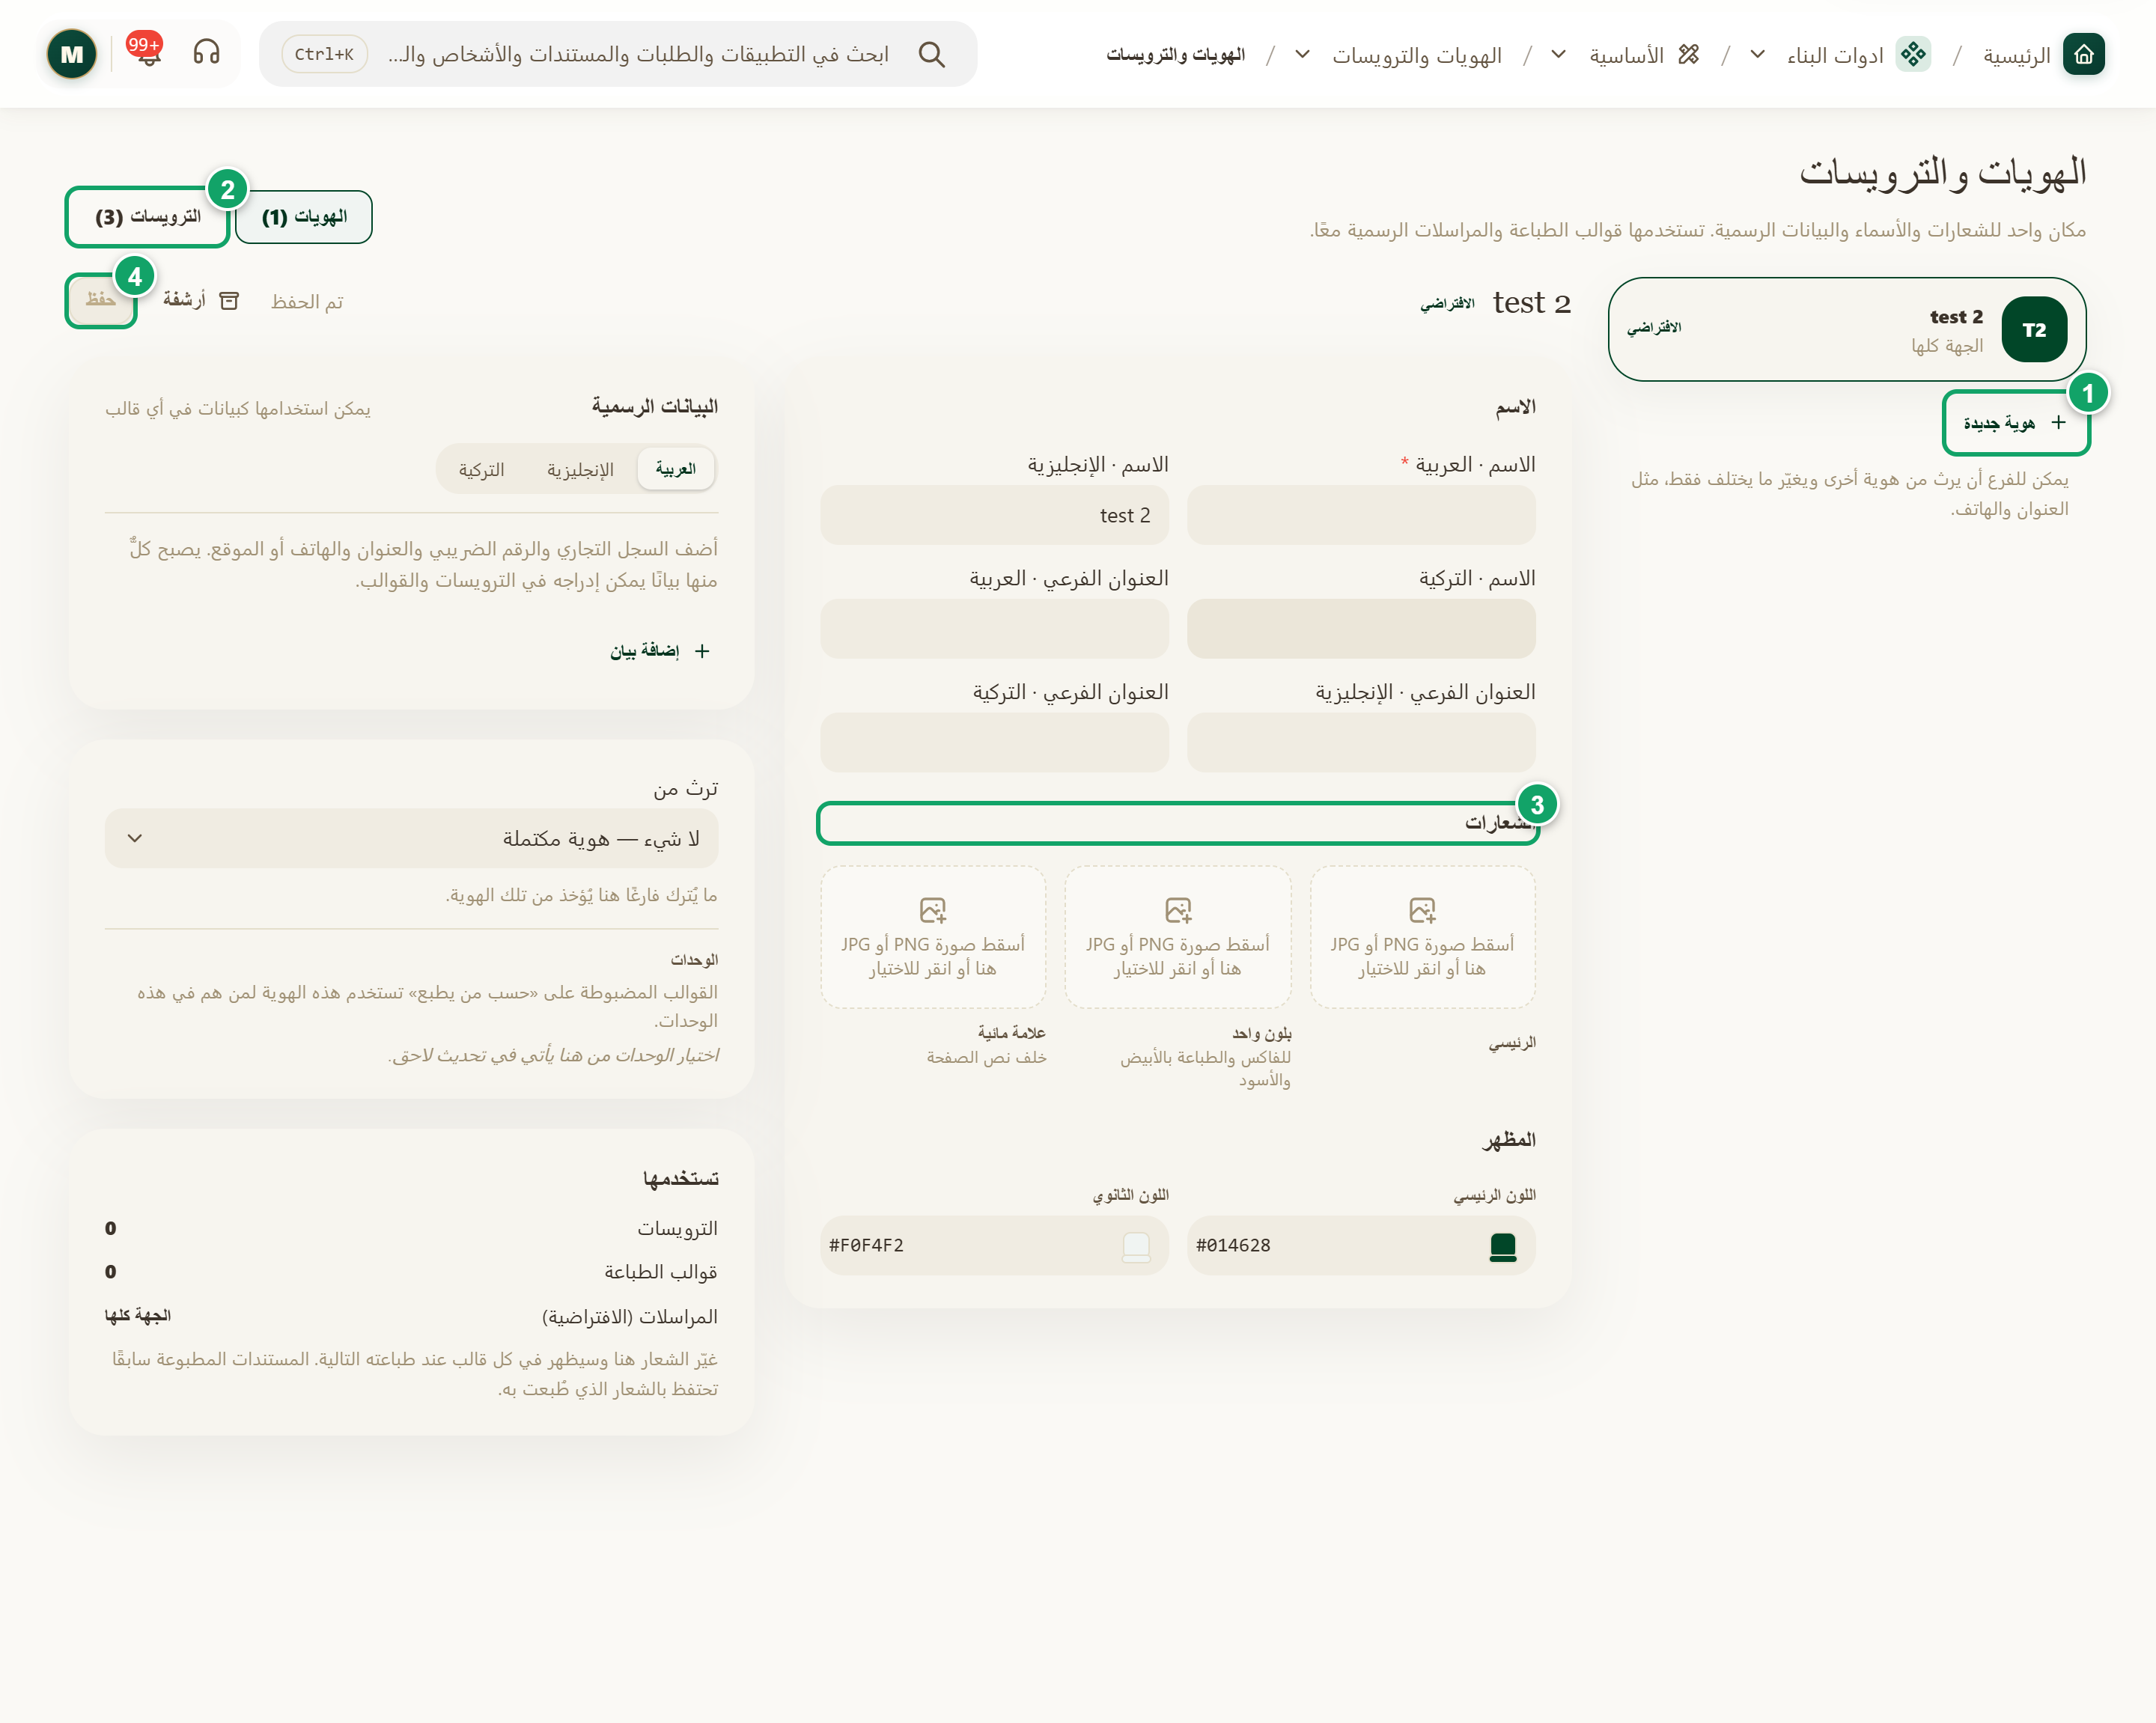
\includegraphics[width=0.95\linewidth,height=0.72\textheight,keepaspectratio]{figures/screens/ch06-identities-ar.png}
\caption{صفحة «الهويات والترويسات»}
\label{fig:builder-identities-screen}
\shotnote{تعرض الصفحة الهوية الافتراضية للمؤسسة وحقولها، وهي هنا هوية مؤسسة الاختبار. ① «هوية جديدة»: تنشئ هوية أخرى، مثل هوية فرع. ② «الترويسات»: تبويب الترويسات المشتركة. ③ «الشعارات»: الشعار الرئيسي وبلون واحد والعلامة المائية. ④ «حفظ»: يحفظ تعديل الهوية.}
\end{figure}


\begin{table}[H]
\centering
\caption{ما الذي تجده هنا؟}
\label{tab:builder-identities-data}
\begin{tabularx}{\linewidth}{R{3.6cm} Y}
\rcHeaderRow
\thh{الجزء} & \thh{المحتوى والإجراء}\\
الهويات & لكل هوية «الاسم» و«العنوان الفرعي» بكل لغة، و«الشعارات» (الرئيسي، بلون واحد، علامة مائية)، و«المظهر» بلونين، و«البيانات الرسمية».\\
ترث من & تجعل الهوية تأخذ ما لم تحدده من هوية أخرى، مثل هوية فرع ترث من هوية المؤسسة.\\
تستخدمها & تبيّن الترويسات وقوالب الطباعة والمراسلات التي تعتمد على الهوية.\\
الترويسات & لكل ترويسة اسم ولغة، وعناصر مثل الشعار وتاريخ الطباعة ورمز QR ورقم الصفحة، وتحديد ظهور الرأس والتذييل في كل صفحة أو الأولى فقط.\\
\end{tabularx}
\end{table}

\begin{figure}[H]
\centering
\begin{tikzpicture}[node distance=0.5cm]
\node[entity] (id) {\RL{الهوية}};
\node[entityOpt,below=0.7cm of id] (lh) {\RL{الترويسة}};
\node[entityOpt,below right=0.7cm and 0.3cm of lh] (print) {\RL{قوالب الطباعة}};
\node[entityOpt,below left=0.7cm and 0.3cm of lh] (corr) {\RL{المراسلات الرسمية}};
\draw[dependsOnOpt] (id) -- (lh);
\draw[dependsOnOpt] (lh.south) -- ++(0,-0.3) -| (print.north);
\draw[dependsOnOpt] (lh.south) -- ++(0,-0.3) -| (corr.north);
\end{tikzpicture}
\rclegend
\caption{من الهوية إلى المستند المطبوع}
\label{fig:builder-identities-model}
\shotnote{يوضّح الشكل أن الهوية تغذّي الترويسة، وأن الترويسة مشتركة بين قوالب الطباعة والمراسلات الرسمية. لذلك عدّل الشعار أو البيانات الرسمية في الهوية مرة واحدة، فيظهر التعديل في كل مستند يُطبع بعد ذلك؛ وراجع «تستخدمها» قبل أي تغيير.}
\end{figure}

\subsection{خطوات العمل والتحقق}
\begin{enumerate}
\item افتح «الهويات والترويسات»، واختر الهوية الافتراضية «الجهة كلها» أو أنشئ «هوية جديدة».
\item اكتب الاسم بكل لغة، وارفع الشعارات بصيغة PNG أو JPG، وأضف البيانات الرسمية، ثم اضغط «حفظ».
\item افتح «الترويسات»، وأنشئ «ترويسة جديدة»، واختر عناصرها ومكان ظهورها.
\end{enumerate}

\textbf{تحقق ومعالجة المشكلة:} اطبع مستنداً تجريبياً من قالب يستخدم الترويسة، فيجب أن يظهر الشعار والبيانات الجديدة. وإذا لم تستطع أرشفة هوية، فاجعل هوية أخرى هي الافتراضية أولاً، لأن الهوية الافتراضية لا تُؤرشف.

\clearpage
\section{لوحات المعلومات}
\label{sec:builder-feature-dashboards}

لوحة المعلومات صفحة أرقام ورسوم بيانية تلخّص العمل، مثل عدد الطلبات المفتوحة أو متوسط مدة الإنجاز. وتبنيها من عناصر تأخذ بياناتها من نوع سجلات أو طلبات نماذج أو غيرهما، ثم تنشرها وتضعها في التنقل. ويرى كل مشاهد البيانات بحسب صلاحياته، فاللوحة لا تتجاوز صلاحيات أحد.

\textbf{المسار ومن يستخدمه:} «ادوات البناء» ← «الأساسية» ← «لوحات المعلومات». يبنيها من يملك صلاحية إنشائها، ويشاهدها من مُنح الوصول إليها.

\begin{rcnote}[مثال: شركة الأفق]
تبني الأفق لوحة «متابعة الزيارات» فيها رقم للطلبات المنتظرة، ورسم بياني للزيارات حسب الفرع، وتقويم بمواعيدها، فتراجعها سارة الخطيب كل أسبوع. وتبدأ اللوحة من ①.
\end{rcnote}

\begin{figure}[H]
\centering
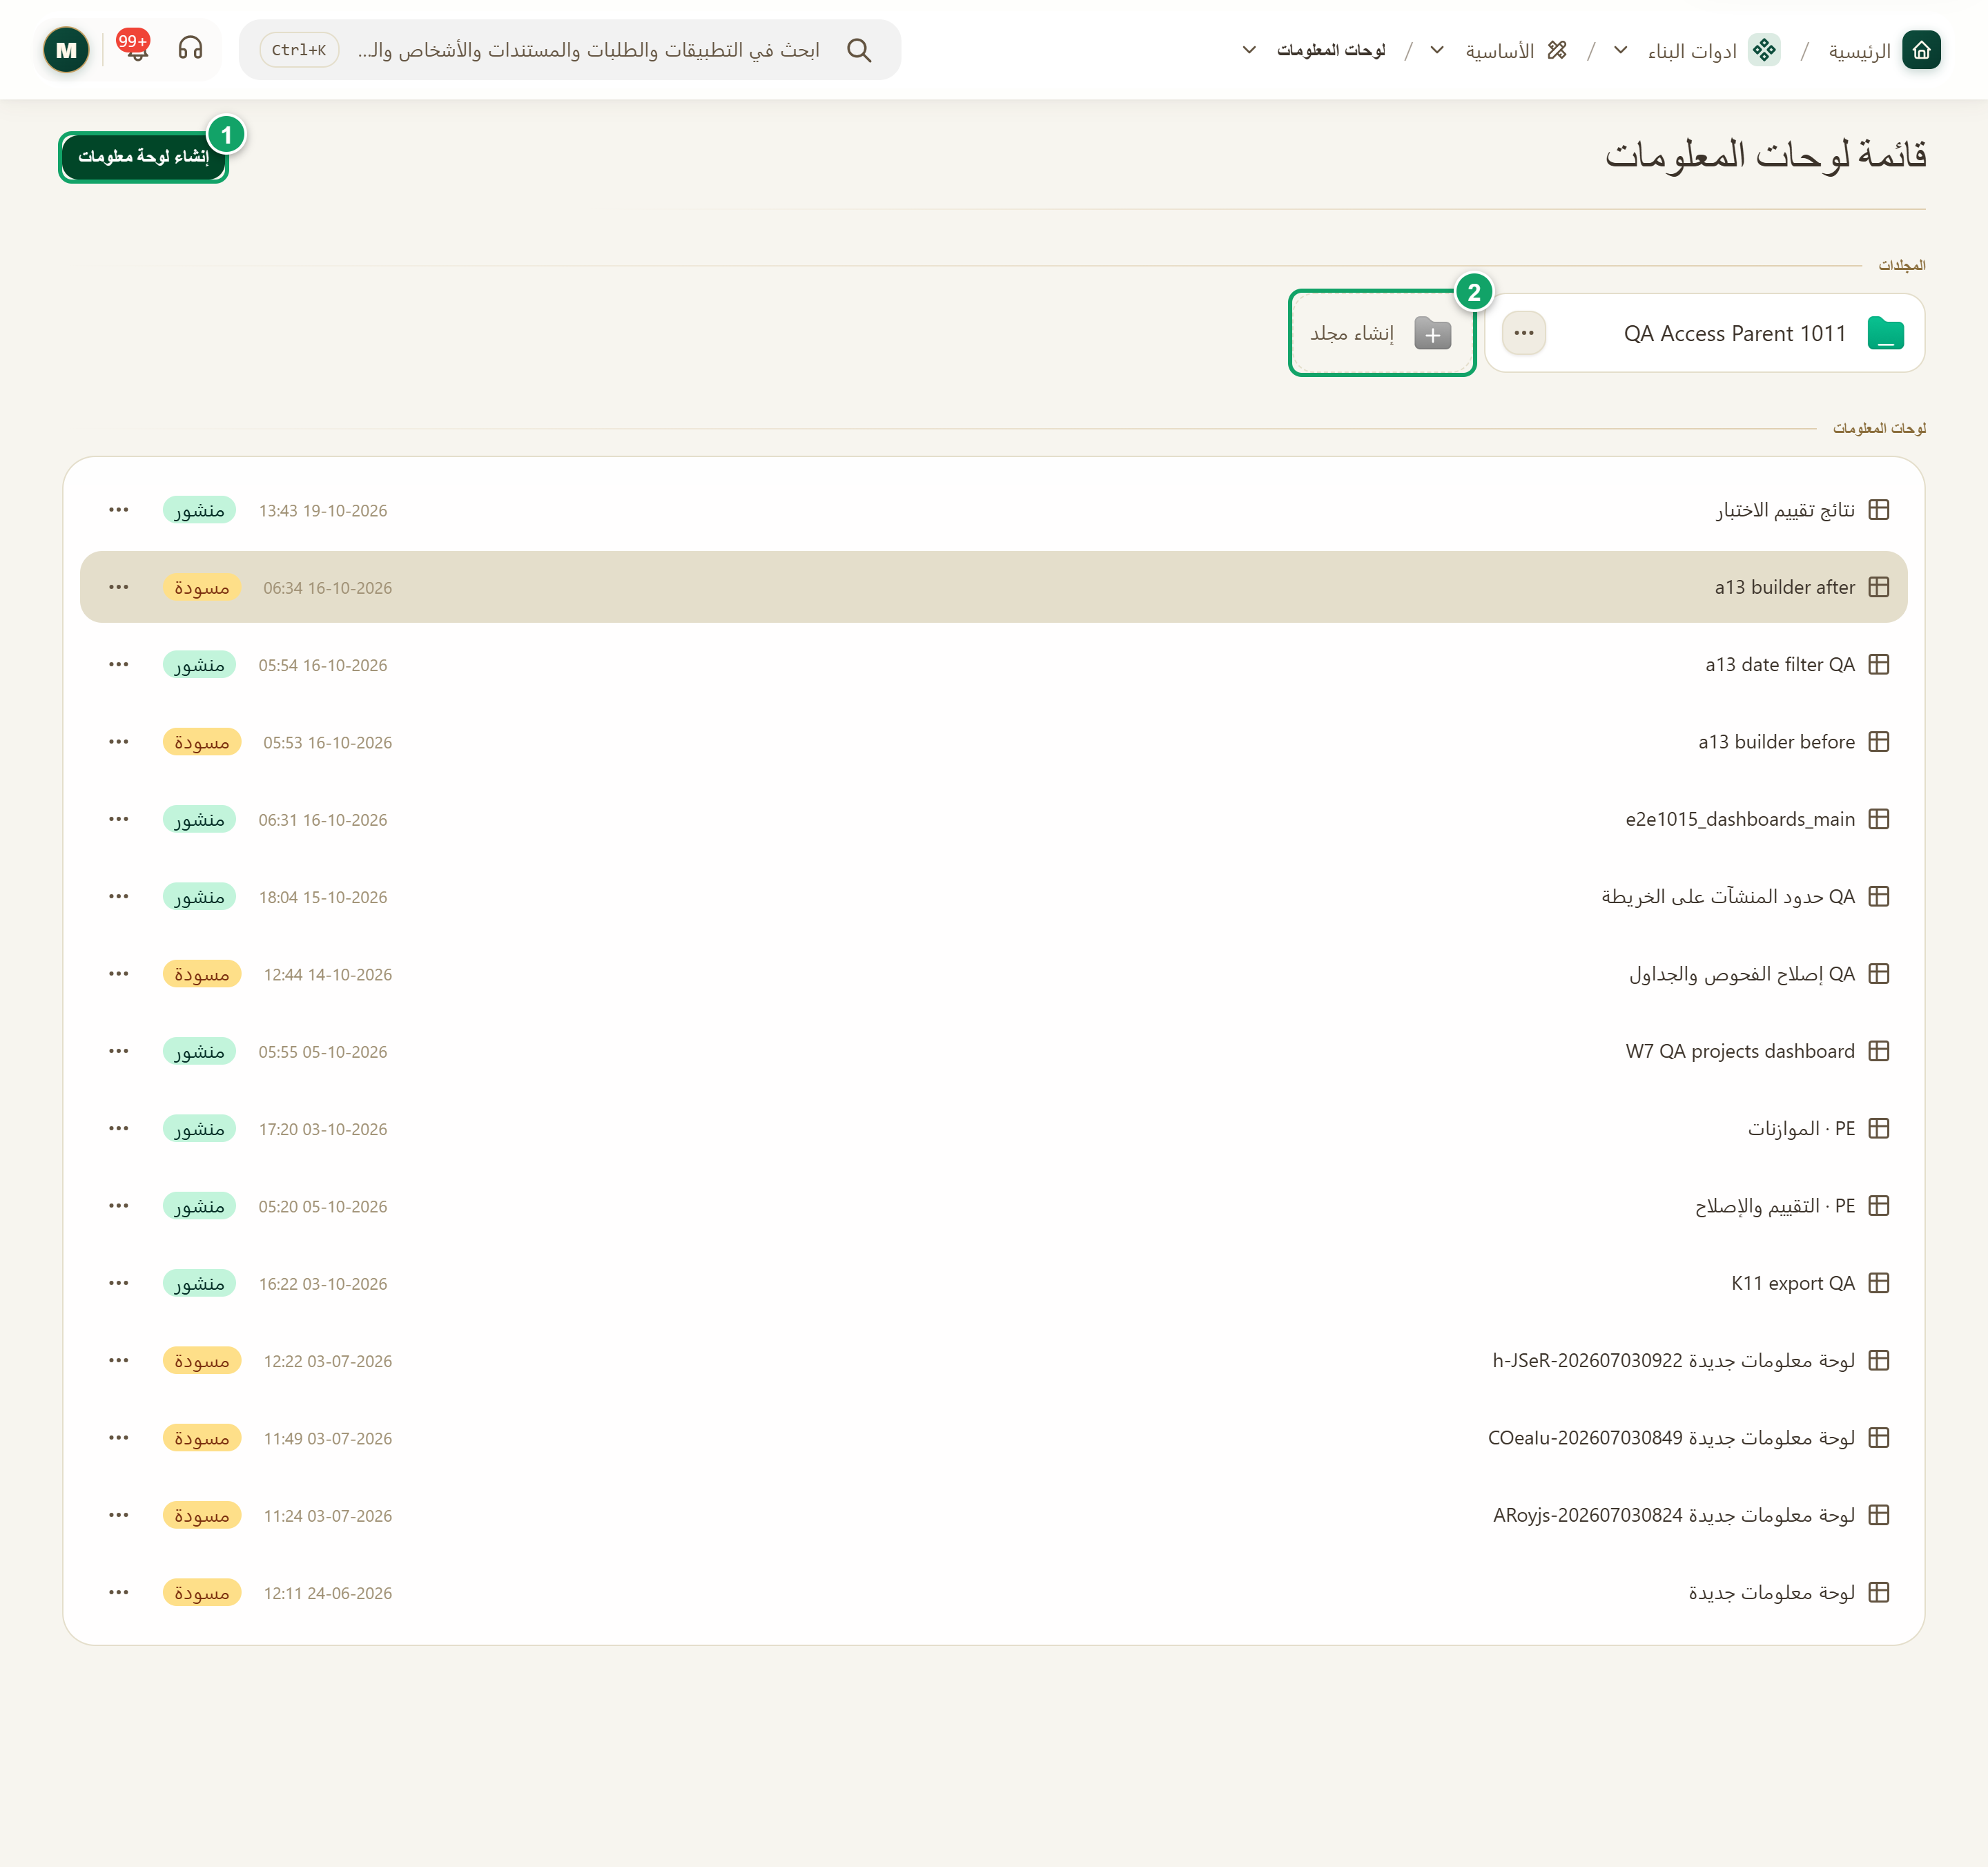
\includegraphics[width=0.95\linewidth,height=0.72\textheight,keepaspectratio]{figures/screens/ch06-dashboards-ar.png}
\caption{صفحة «لوحات المعلومات»}
\label{fig:builder-dashboards-screen}
\shotnote{تعرض الصفحة المجلدات ولوحات المعلومات مع حالتها، وهي هنا لوحات اختبار. ① «إنشاء لوحة معلومات»: تبدأ لوحة جديدة. ② «إنشاء مجلد»: ينظّم اللوحات في مجلدات.}
\end{figure}


\begin{table}[H]
\centering
\caption{ما الذي تجده هنا؟}
\label{tab:builder-dashboards-data}
\begin{tabularx}{\linewidth}{R{3.6cm} Y}
\rcHeaderRow
\thh{الجزء} & \thh{المحتوى والإجراء}\\
قائمة لوحات المعلومات & اللوحات والمجلدات مع حالتها «مسودة» أو «منشور»، وزر «إنشاء لوحة معلومات» و«إنشاء مجلد».\\
العناصر & «إضافة قسم» ثم «إضافة عنصر»: رسم بياني، ورقم، ومؤشر أداء، وجدول، وتقدم، وتقويم، وخريطة، وغيرها.\\
مصدر البيانات & كيان، أو طلبات النماذج، أو إجراء تشغيلي، أو بيانات يدوية وغيرها، مع مستوى الوصول للبيانات.\\
المرشحات & تتيح للمشاهد تغيير نطاق التاريخ للوحة كلها أو لأقسام أو عناصر محددة.\\
الإعدادات والوصول & الاسم والوصف و«إظهار في التنقل» والتطبيق والقسم، و«إدارة الوصول» لتحديد من يشاهدها.\\
الإصدارات والنشر & «نشر» يُنشئ إصداراً جديداً يحل محل المنشور، و«سجل الإصدارات» للاستعادة.\\
\end{tabularx}
\end{table}

\begin{figure}[H]
\centering
\begin{tikzpicture}[node distance=0.5cm]
\node[stepBox] (a) {\RL{إنشاء لوحة معلومات}};
\node[stepBox,below=of a] (b) {\RL{أقسام وعناصر ومصادر}};
\node[stepBox,below=of b] (c) {\RL{معاينة ومقارنة بسجلات معروفة}};
\node[stepBox,below=of c] (d) {\RL{نشر وإظهار في التنقل}};
\draw[flowsTo] (a) -- (b);
\draw[flowsTo] (b) -- (c);
\draw[flowsTo] (c) -- (d);
\end{tikzpicture}
\rclegend
\caption{بناء لوحة معلومات}
\label{fig:builder-dashboards-flow}
\shotnote{يضع المخطط المقارنة بسجلات معروفة قبل النشر، لأن الرقم الخاطئ في لوحة يقود إلى قرار خاطئ. فإذا كنت تعرف أن خمسة طلبات تنتظر القرار، فيجب أن يعرض العنصر خمسة. ولا يرى الفريق اللوحة في التنقل قبل نشرها.}
\end{figure}

\subsection{خطوات العمل والتحقق}
\begin{enumerate}
\item افتح «لوحات المعلومات» واضغط «إنشاء لوحة معلومات»، ثم اكتب الاسم ووصفاً واضحاً.
\item أضف قسماً، ثم عنصراً، واختر له مصدر البيانات والحقول والمرشحات، واكتب عنواناً يوضح ما يعدّه.
\item اضغط «معاينة» وقارن الأرقام بسجلات تعرفها، ثم حدد في الإعدادات مكان ظهورها واضغط «نشر».
\end{enumerate}

\textbf{تحقق ومعالجة المشكلة:} افتح اللوحة من التنقل بصفة مشاهد، فيجب أن تعرض الأرقام المتوقعة. فإذا ظهرت رسالة «لم يتم نشر لوحة المعلومات بعد»، فانشرها؛ وإذا رأى مستخدم أرقاماً أقل من غيره، فذلك لأن اللوحة تعرض ما تسمح به صلاحياته.

\clearpage
\section{الصفحات}
\label{sec:builder-feature-pages}

الصفحة تضع لوحة معلومات محفوظة من مساحة التحليلات بالذكاء الاصطناعي (\en{DB Genie}) داخل قسم في تطبيق، فتظهر للأعضاء عنصراً في القائمة. وهي الطريقة لمشاركة لوحة صنعتها في «لوحات معلومات الذكاء الاصطناعي» مع الفريق.

\textbf{المسار ومن يستخدمه:} «ادوات البناء» ← «الأساسية» ← «الصفحات». تظهر لمالك المؤسسة ومسؤولها فقط.

\begin{rcnote}[مثال: شركة الأفق]
يصنع مسؤول النظام لوحة تحليل لمدد إنجاز الزيارات في مساحة الذكاء الاصطناعي، ثم ينشرها صفحةً في قسم «الزيارات» داخل «خدمات الفروع» لتراها سارة الخطيب. وتبدأ الصفحة من ①.
\end{rcnote}

\begin{figure}[H]
\centering
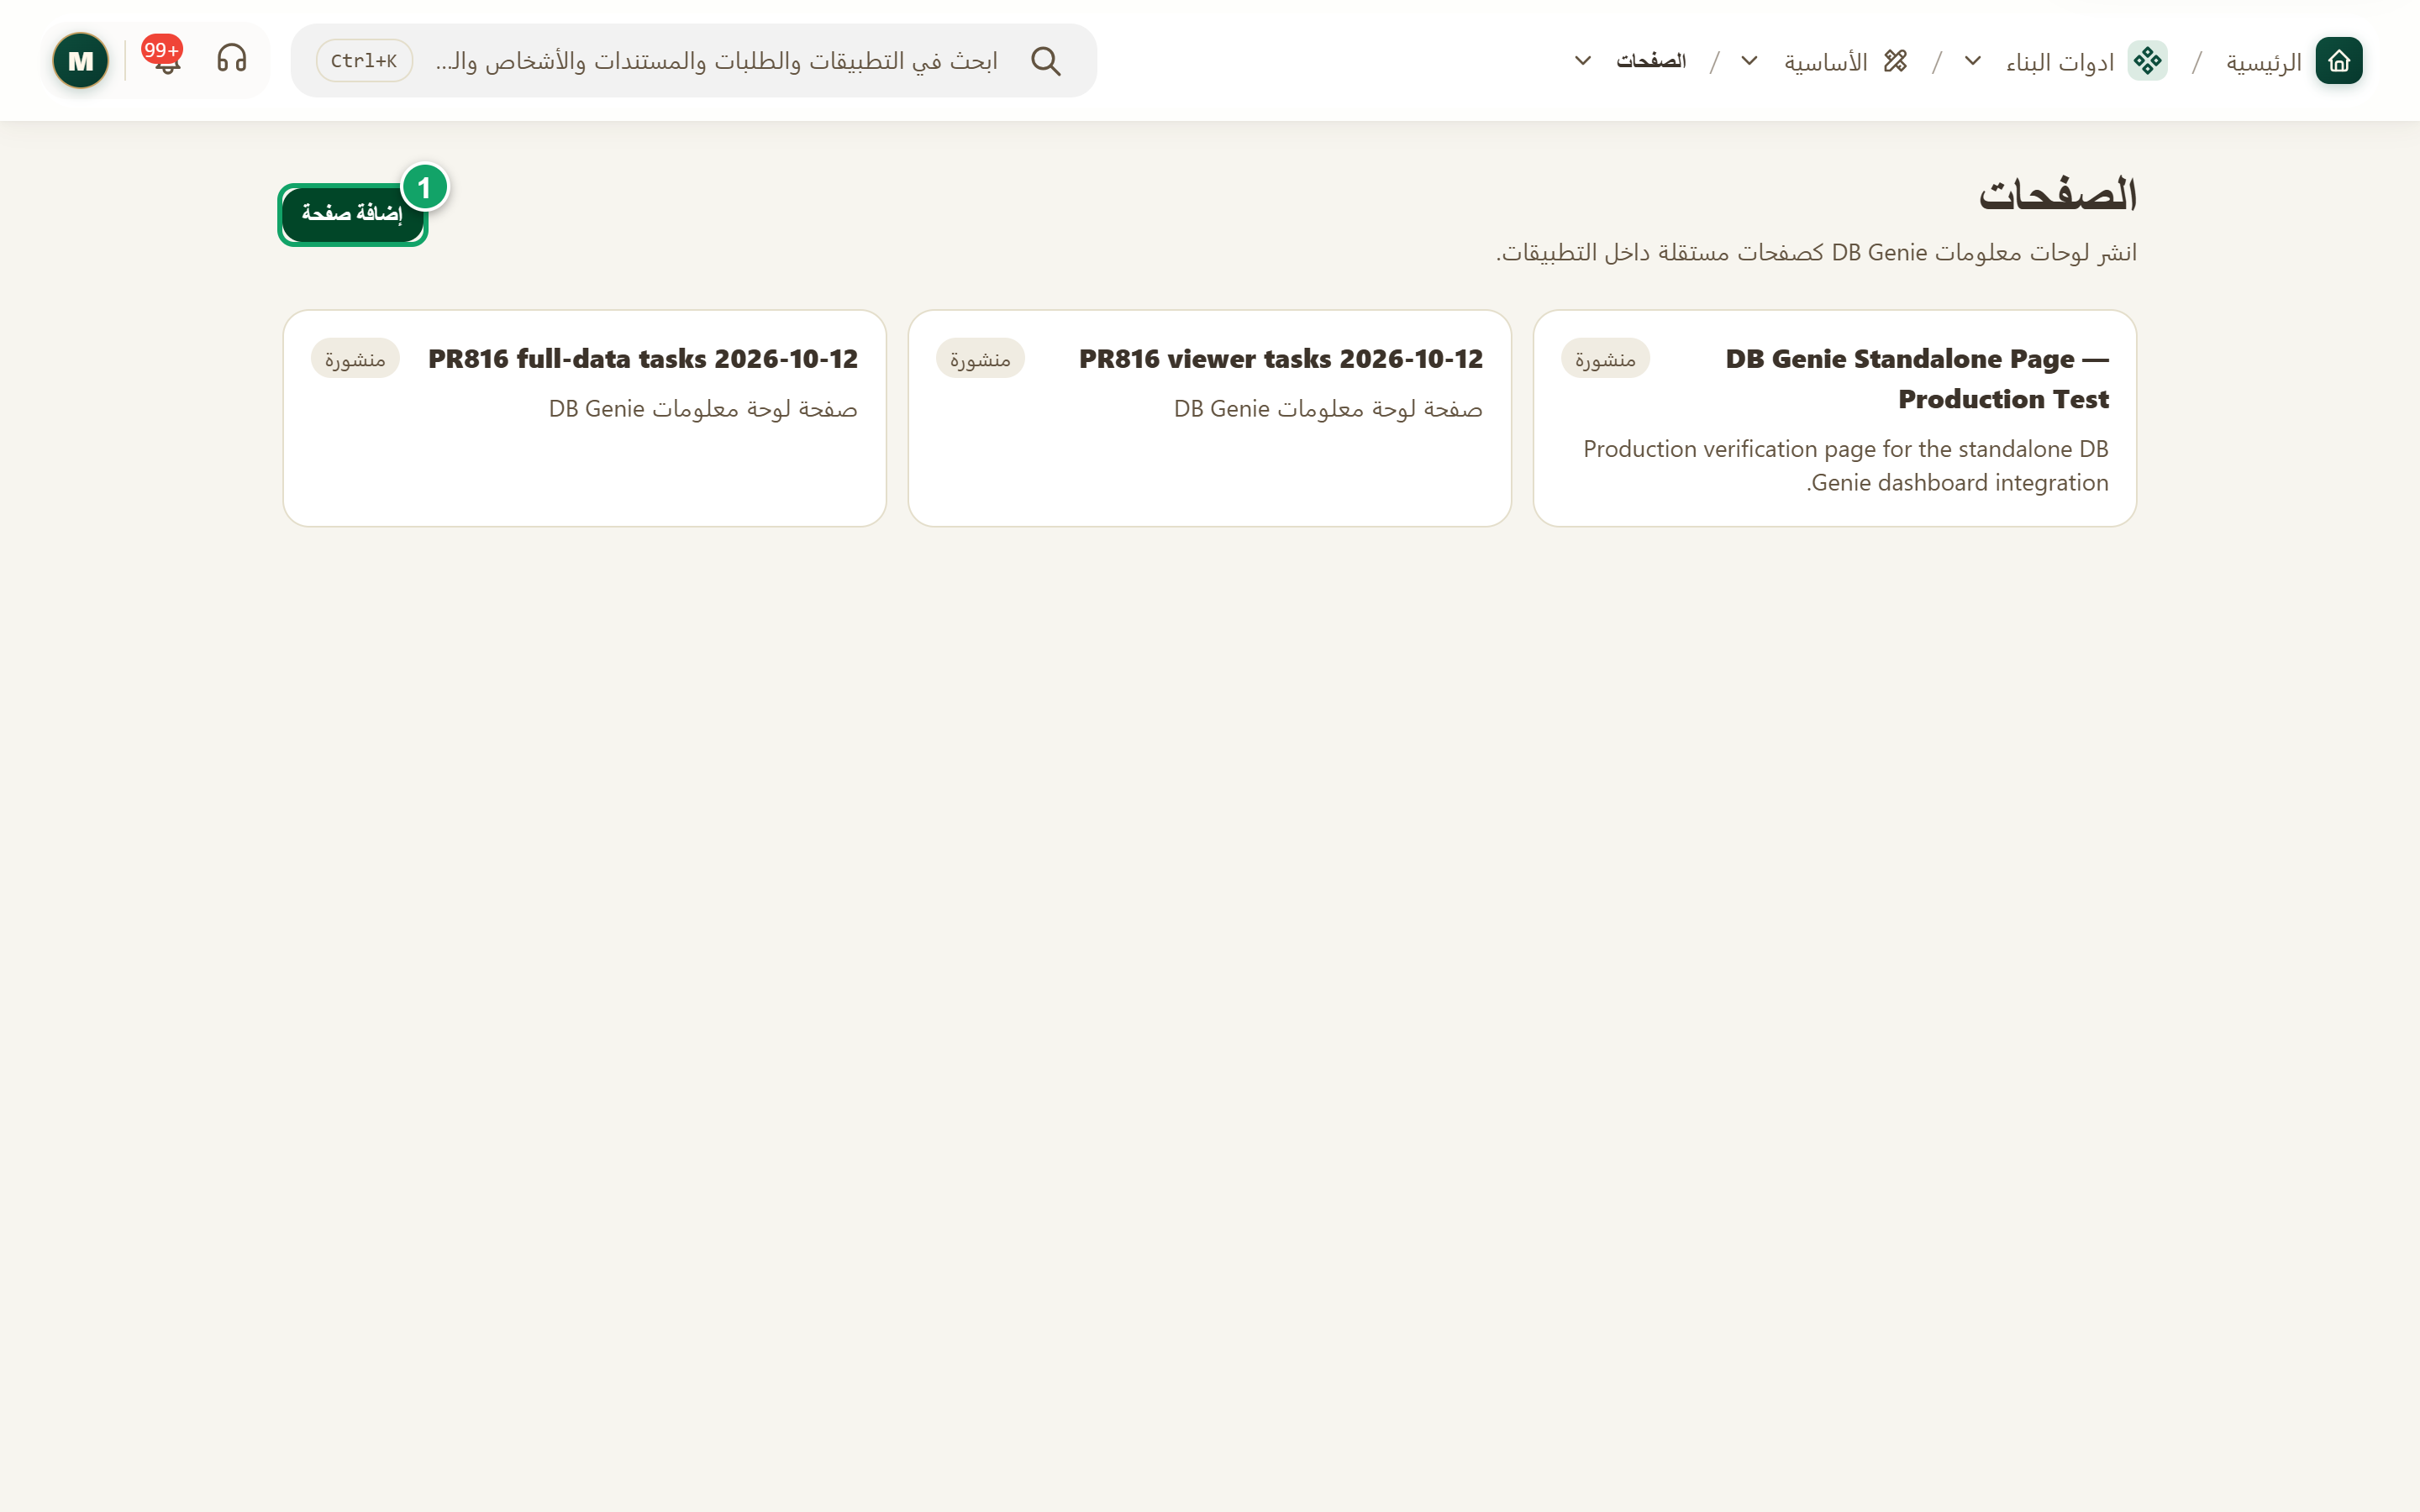
\includegraphics[width=0.95\linewidth,height=0.72\textheight,keepaspectratio]{figures/screens/ch06-pages-ar.png}
\caption{صفحة «الصفحات»}
\label{fig:builder-pages-screen}
\shotnote{تعرض الصفحة الصفحات المستقلة المنشورة في التطبيقات، وهي هنا صفحات اختبار. ① «إضافة صفحة»: تبدأ صفحة جديدة تختار لها اللوحة والتطبيق والقسم.}
\end{figure}


\begin{table}[H]
\centering
\caption{حقول الصفحة}
\label{tab:builder-pages-data}
\begin{tabularx}{\linewidth}{R{3.6cm} Y}
\rcHeaderRow
\thh{الحقل} & \thh{المعنى}\\
العنوان والوصف & اسم الصفحة كما يظهر في القائمة، ووصف قصير.\\
التطبيق والقسم & المكان الذي تظهر فيه الصفحة في التنقل.\\
لوحة معلومات DB Genie & لوحة محفوظة تختارها بزر «اختيار لوحة معلومات».\\
البيانات المعروضة & «بصلاحيات المشاهد» وهو الأكثر أماناً، أو بيانات المؤسسة بحماية، أو بيانات المؤسسة كاملة دون تحقق من نطاق المشاهد.\\
الحالة & «مسودة» أو «منشورة» أو «مؤرشفة». ولا تظهر الصفحة في التنقل إلا وهي منشورة.\\
\end{tabularx}
\end{table}

\begin{figure}[H]
\centering
\begin{tikzpicture}[node distance=0.5cm]
\node[stepBox] (a) {\RL{لوحة في مساحة الذكاء الاصطناعي}};
\node[stepBox,below=of a] (b) {\RL{إضافة صفحة واختيار اللوحة}};
\node[stepBox,below=of b] (c) {\RL{الحالة: منشورة}};
\node[stepBox,below=of c] (d) {\RL{منح صلاحية العرض للأدوار}};
\draw[flowsTo] (a) -- (b);
\draw[flowsTo] (b) -- (c);
\draw[flowsTo] (c) -- (d);
\end{tikzpicture}
\rclegend
\caption{من لوحة خاصة إلى صفحة للفريق}
\label{fig:builder-pages-flow}
\shotnote{يبيّن المخطط أن نشر الصفحة وحده لا يكفي ليراها الأعضاء، بل يحتاج كل دور إلى صلاحية عرض الصفحة في إعدادات الأدوار. وتبقى اللوحة الأصلية كما هي، فحذف الصفحة لا يحذف اللوحة.}
\end{figure}

\subsection{خطوات العمل والتحقق}
\begin{enumerate}
\item احفظ اللوحة في «لوحات معلومات الذكاء الاصطناعي» أولاً.
\item افتح «الصفحات» واضغط «إضافة صفحة»، ثم اكتب العنوان واختر التطبيق والقسم واللوحة.
\item اختر «بصلاحيات المشاهد» في «البيانات المعروضة»، واجعل الحالة «منشورة»، ثم اضغط «حفظ الصفحة».
\item امنح الأدوار المناسبة صلاحية عرض الصفحة من إعدادات الأدوار.
\end{enumerate}

\textbf{تحقق ومعالجة المشكلة:} يجب أن تظهر الصفحة في القسم الذي اخترته لمن يملك صلاحية عرضها. فإذا ظهرت رسالة «العنوان والتطبيق والقسم ولوحة المعلومات مطلوبة»، فأكمل الحقول الأربعة. وإذا لم يرها عضو، فراجع حالتها وصلاحية دوره.

\clearpage
\section{لوحات معلومات الذكاء الاصطناعي}
\label{sec:builder-feature-ai-dashboards}

تفتح هذه الصفحة مساحة التحليلات بالذكاء الاصطناعي (\en{DB Genie})، حيث تصف ما تريد معرفته فتُبنى لك لوحة معلومات من بيانات المؤسسة. وتكون المساحة خاصة بك، ولا تستخدم إلا البيانات التي تستطيع قراءتها. ولمشاركة لوحة مع الفريق، انشرها من صفحة «الصفحات».

\textbf{المسار ومن يستخدمه:} «ادوات البناء» ← «الأساسية» ← «لوحات معلومات الذكاء الاصطناعي». تظهر لمن يتضمن مقعده التحليلات، إذا كان مسؤولاً في المؤسسة أو يملك صلاحية عرض لوحات المعلومات.

\begin{rcnote}[مثال: شركة الأفق]
تطلب سارة الخطيب لوحة توضح عدد الزيارات لكل فرع في كل شهر، فتراجع النتيجة في مساحتها الخاصة قبل أن يقرر مسؤول النظام نشرها صفحةً للفريق. وتطلب سارة اللوحة داخل المساحة ①.
\end{rcnote}

\begin{figure}[H]
\centering
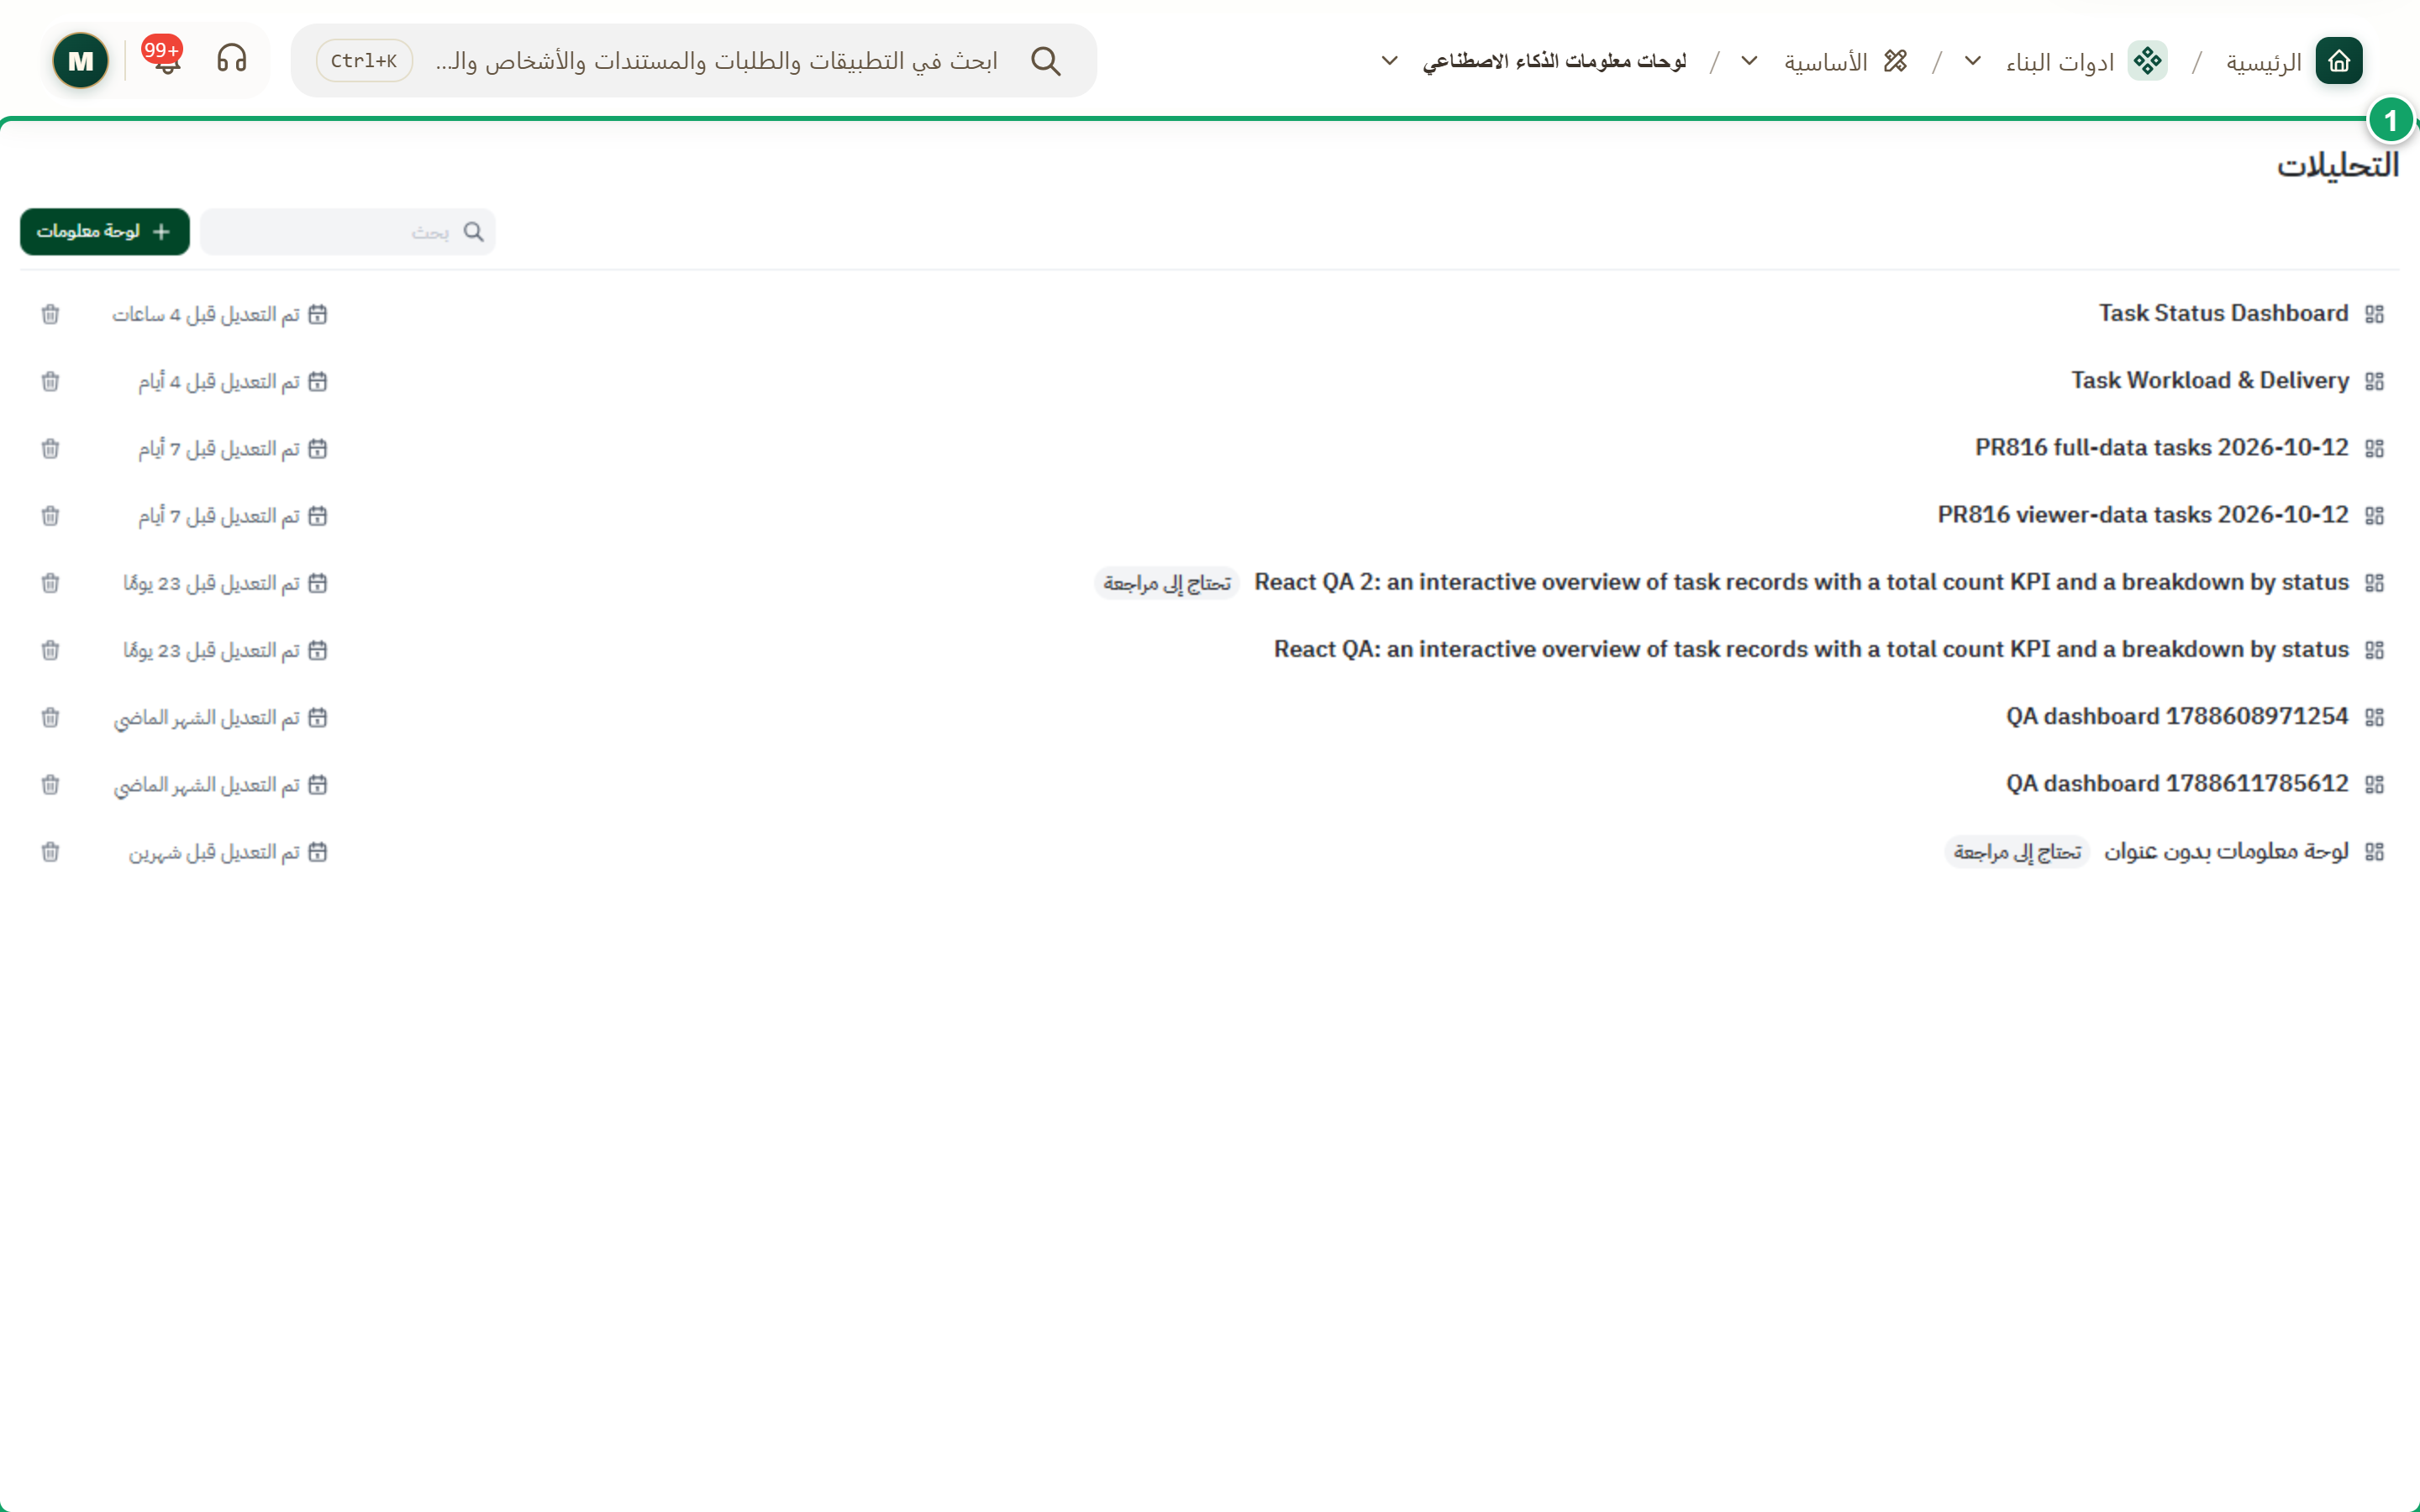
\includegraphics[width=0.95\linewidth,height=0.72\textheight,keepaspectratio]{figures/screens/ch06-ai-dashboards-ar.png}
\caption{مساحة «لوحات معلومات الذكاء الاصطناعي»}
\label{fig:builder-ai-dashboards-screen}
\shotnote{تُفتح مساحة التحليلات داخل كيان، وتعرض لوحات المستخدم الخاصة به. والمحتوى هنا محتوى مؤسسة الاختبار. ① مساحة التحليلات: فيها تُنشأ اللوحات وتُراجَع، ويخدمها نظام التحليلات المضمّن.}
\end{figure}


\begin{table}[H]
\centering
\caption{ما الذي يجب معرفته؟}
\label{tab:builder-ai-dashboards-data}
\begin{tabularx}{\linewidth}{R{3.6cm} Y}
\rcHeaderRow
\thh{الجانب} & \thh{المعنى}\\
مساحة خاصة & اللوحات هنا لك وحدك، وتُحسب من البيانات التي تملك صلاحية قراءتها فقط.\\
بيانات غير متاحة & قد تظهر رسالة بأن بعض البيانات غير متاحة لأن صلاحياتك على أنواع سجلات معينة أوسع من أن تُضمَّن.\\
المشاركة & تُشارك اللوحة بنشرها صفحةً من «الصفحات»، لا من هذه المساحة.\\
\end{tabularx}
\end{table}

\begin{figure}[H]
\centering
\begin{tikzpicture}[node distance=0.5cm]
\node[stepBox] (a) {\RL{وصف ما تريد معرفته}};
\node[stepBox,below=of a] (b) {\RL{مراجعة اللوحة الناتجة}};
\node[stepBox,below=of b] (c) {\RL{نشرها من الصفحات عند الحاجة}};
\draw[flowsTo] (a) -- (b);
\draw[flowsTo] (b) -- (c);
\end{tikzpicture}
\rclegend
\caption{من سؤال إلى لوحة مشتركة}
\label{fig:builder-ai-dashboards-flow}
\shotnote{يضع المخطط المراجعة قبل المشاركة، لأن اللوحة التي يولّدها الذكاء الاصطناعي قد تفهم السؤال على غير ما تقصد. فقارن أرقامها بما تعرفه، ثم شاركها عبر «الصفحات» فقط عندما تثق بها.}
\end{figure}

\subsection{خطوات العمل والتحقق}
\begin{enumerate}
\item افتح «لوحات معلومات الذكاء الاصطناعي»، وانتظر حتى تُحمَّل مساحة التحليلات.
\item أنشئ لوحة جديدة واكتب ما تريد معرفته بوضوح، مع الفترة والحقول المهمة.
\item راجع اللوحة واحفظها، ثم انشرها من «الصفحات» إن أردت أن يراها الفريق.
\end{enumerate}

\textbf{تحقق ومعالجة المشكلة:} يجب أن تُفتح المساحة وتعرض لوحاتك. فإذا ظهرت رسالة «تعذر فتح التحليلات» أو أعادتك الصفحة إلى الرئيسية، فمقعدك لا يتضمن التحليلات أو تنقصك صلاحية عرض لوحات المعلومات؛ فاطلبها من مسؤول المؤسسة.

\clearpage
\section{تقارير الذكاء الاصطناعي}
\label{sec:builder-feature-ai-reports}

تفتح هذه الصفحة مساحة التحليلات نفسها في وضع المحادثة: تسأل بلغتك عن بيانات المؤسسة، فيجيبك الذكاء الاصطناعي بتقرير مكتوب وأرقام. وتناسب الأسئلة السريعة التي لا تحتاج إلى لوحة دائمة، مثل «كم زيارة أُلغيت هذا الشهر ولماذا؟».

\textbf{المسار ومن يستخدمه:} «ادوات البناء» ← «الأساسية» ← «تقارير الذكاء الاصطناعي». شروط ظهورها هي شروط «لوحات معلومات الذكاء الاصطناعي» نفسها.

\begin{rcnote}[مثال: شركة الأفق]
تسأل سارة الخطيب عن الفروع التي تأخرت زياراتها أكثر من أسبوع، فتحصل على تقرير قصير تبني عليه نقاش الاجتماع الشهري. وتطرح سارة سؤالها في المنطقة ①.
\end{rcnote}

\begin{figure}[H]
\centering
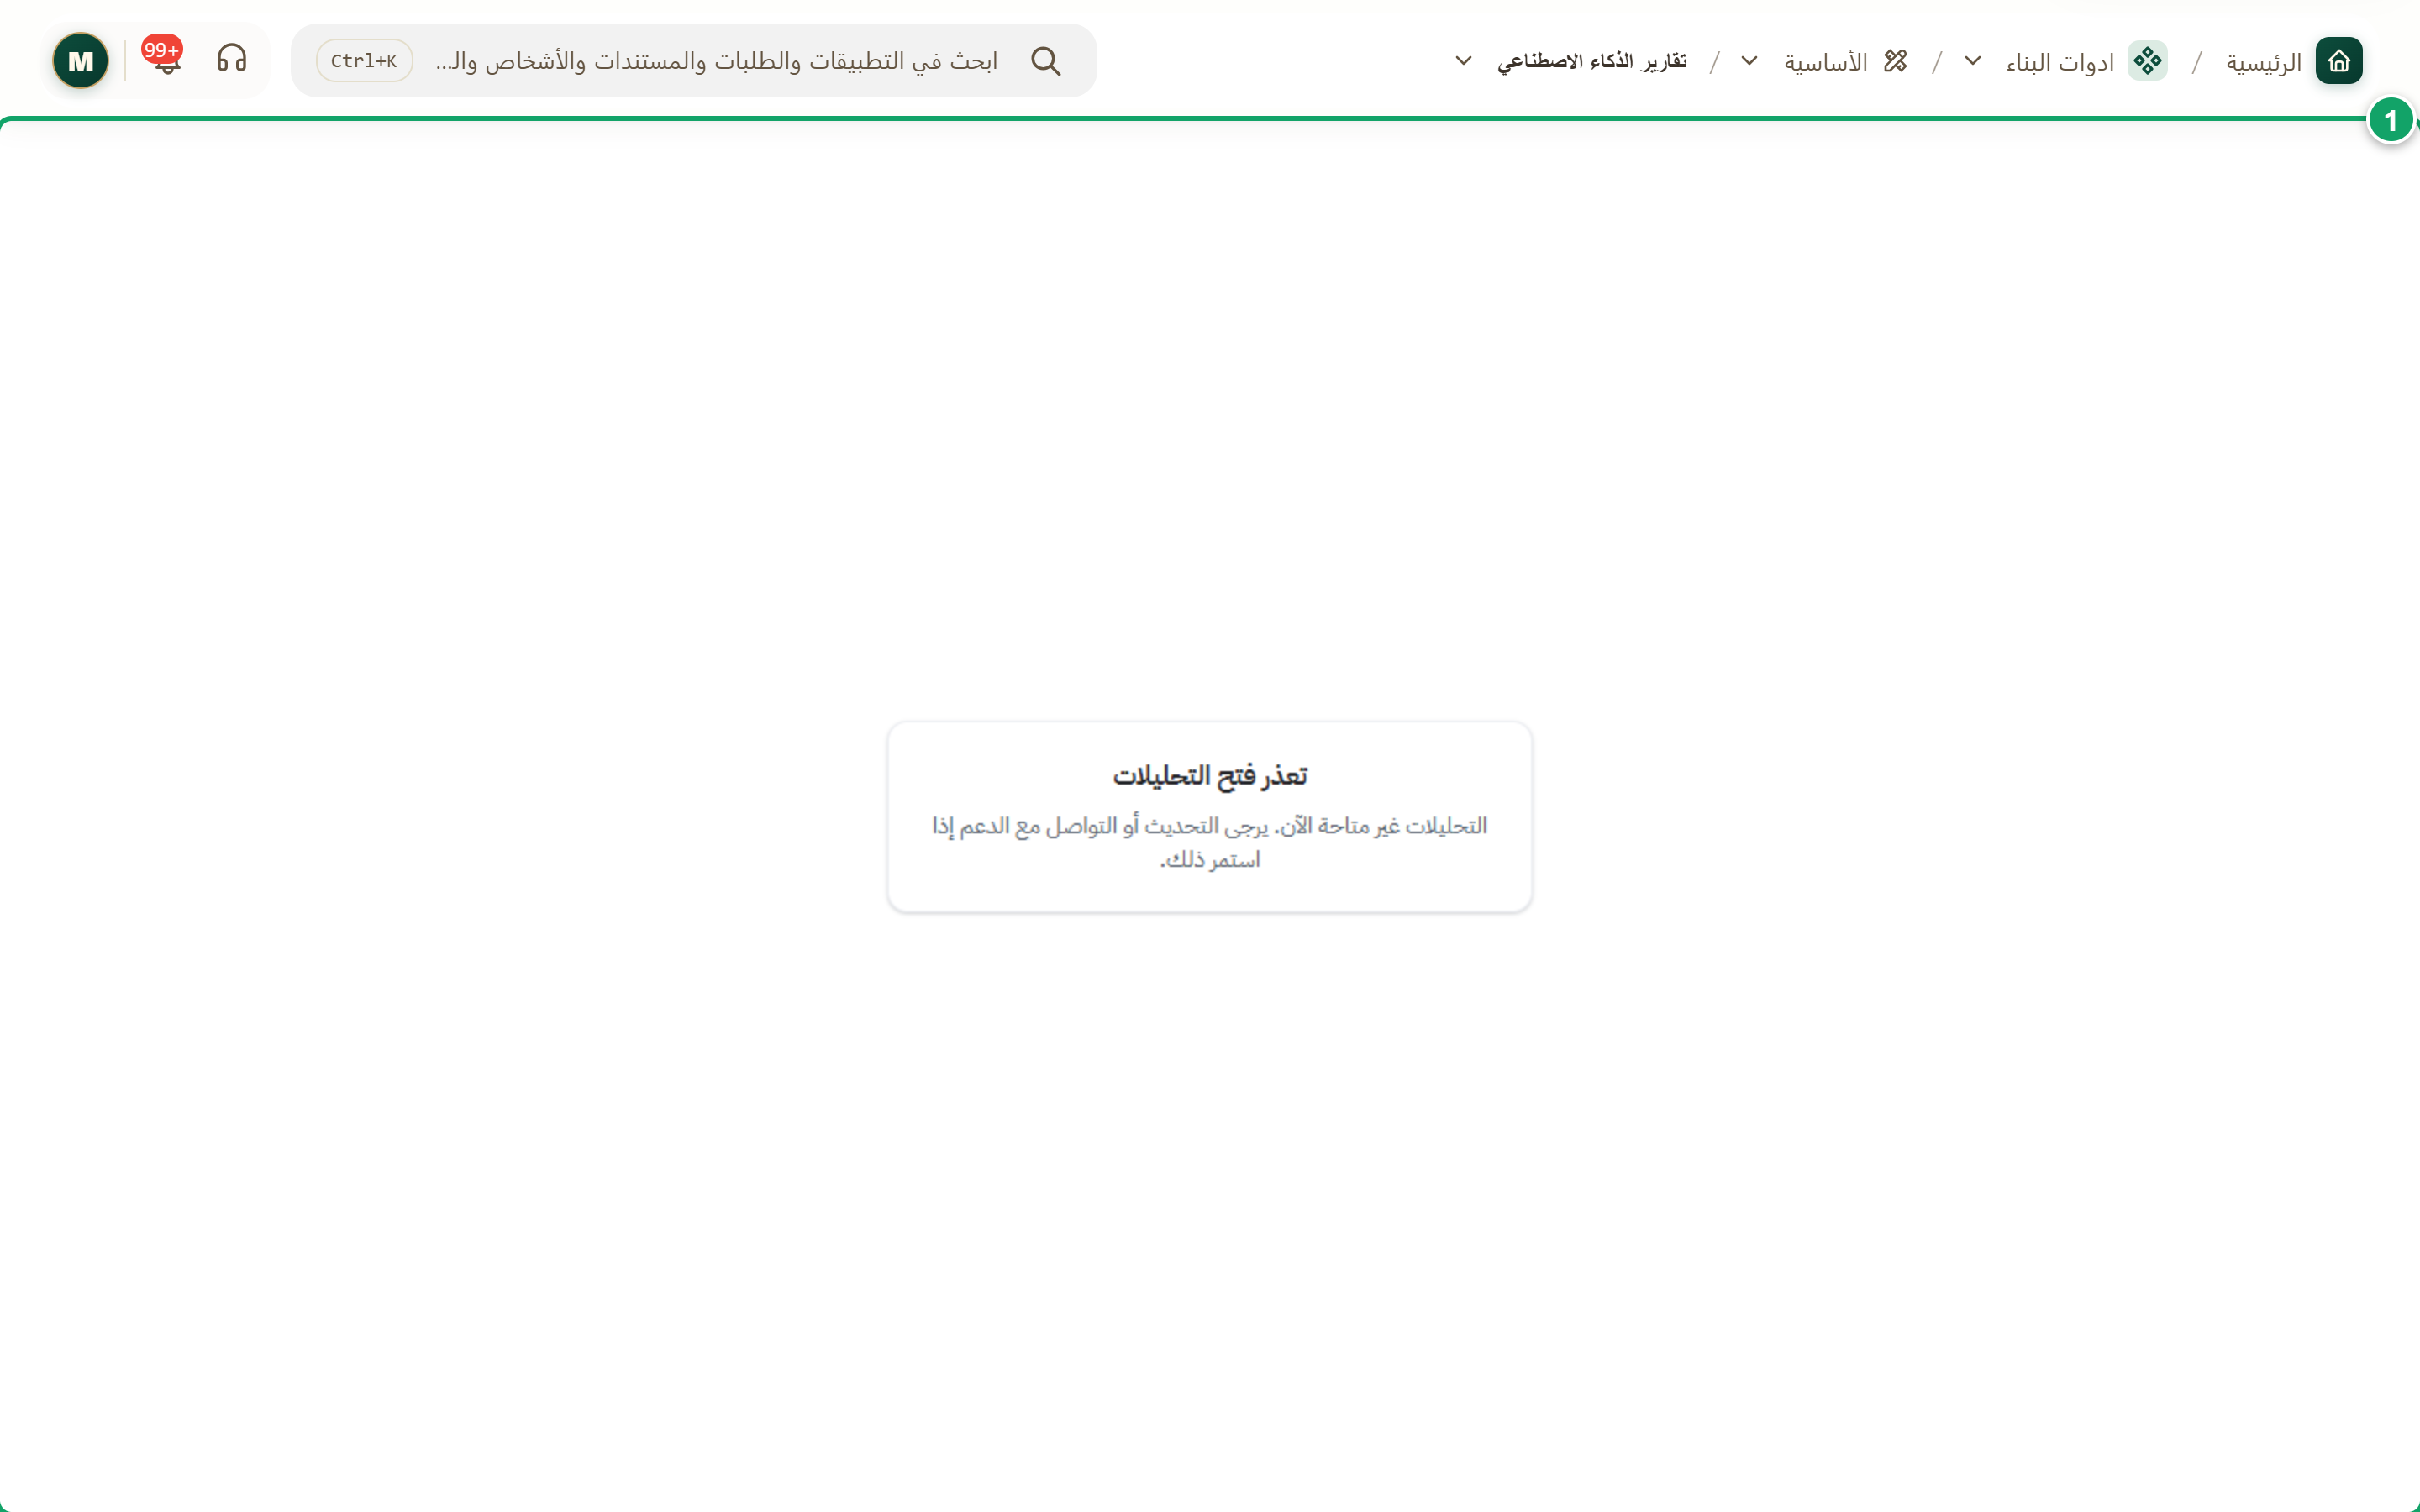
\includegraphics[width=0.95\linewidth,height=0.72\textheight,keepaspectratio]{figures/screens/ch06-ai-reports-ar.png}
\caption{مساحة «تقارير الذكاء الاصطناعي»}
\label{fig:builder-ai-reports-screen}
\shotnote{تُفتح مساحة التحليلات نفسها في وضع المحادثة. ① منطقة المحادثة: تكتب فيها سؤالك وتقرأ التقرير.}
\end{figure}


\begin{table}[H]
\centering
\caption{متى تستخدم التقارير ومتى تستخدم اللوحات؟}
\label{tab:builder-ai-reports-data}
\begin{tabularx}{\linewidth}{R{3.6cm} Y}
\rcHeaderRow
\thh{الحاجة} & \thh{الأنسب}\\
سؤال لمرة واحدة & «تقارير الذكاء الاصطناعي»: اسأل واقرأ الإجابة.\\
متابعة متكررة & «لوحات معلومات الذكاء الاصطناعي» أو «لوحات المعلومات»، لأن اللوحة تُحدَّث وتُراجع دورياً.\\
مشاركة مع الفريق & انشر اللوحة من «الصفحات»؛ فإجابات المحادثة لا تظهر في التنقل.\\
\end{tabularx}
\end{table}

\begin{figure}[H]
\centering
\begin{tikzpicture}[node distance=0.5cm]
\node[stepBox] (a) {\RL{سؤال واضح بفترة محددة}};
\node[stepBox,below=of a] (b) {\RL{قراءة التقرير}};
\node[stepBox,below=of b] (c) {\RL{التحقق من رقم معروف}};
\draw[flowsTo] (a) -- (b);
\draw[flowsTo] (b) -- (c);
\end{tikzpicture}
\rclegend
\caption{طرح سؤال والتحقق من الإجابة}
\label{fig:builder-ai-reports-flow}
\shotnote{ينتهي المخطط بالتحقق، لأن الإجابة مبنية على البيانات التي يستطيع السائل قراءتها وعلى فهم الذكاء الاصطناعي للسؤال. فإذا طابق رقم واحد تعرفه ما في التقرير، زادت ثقتك ببقية الإجابة.}
\end{figure}

\subsection{خطوات العمل والتحقق}
\begin{enumerate}
\item افتح «تقارير الذكاء الاصطناعي»، وانتظر حتى تُحمَّل المحادثة.
\item اكتب سؤالك مع الفترة الزمنية ونوع السجلات المقصود.
\item اقرأ التقرير، وقارن رقماً منه بما تعرفه قبل الاعتماد عليه.
\end{enumerate}

\textbf{تحقق ومعالجة المشكلة:} يجب أن تصل إجابة تشير إلى بيانات مؤسستك. فإذا لم تُفتح الصفحة، فراجع مقعدك وصلاحياتك كما في «لوحات معلومات الذكاء الاصطناعي». وإذا بدت الإجابة ناقصة، فأعد صياغة السؤال بتحديد نوع السجلات والفترة.
